%%%%%%%%%%%%%%%%%%%%%%%%%%%%%%%%%%%%%%%%%
% University Assignment Title Page 
% LaTeX Template
% Version 1.0 (27/12/12)
%
% This template has been downloaded from:
% http://www.LaTeXTemplates.com
%
% Original author:
% WikiBooks (http://en.wikibooks.org/wiki/LaTeX/Title_Creation)
%
% License:
% CC BY-NC-SA 3.0 (http://creativecommons.org/licenses/by-nc-sa/3.0/)
% 
% Instructions for using this template:
% This title page is capable of being compiled as is. This is not useful for 
% including it in another document. To do this, you have two options: 
%
% 1) Copy/paste everything between \begin{document} and \end{document} 
% starting at \begin{titlepage} and paste this into another LaTeX file where you 
% want your title page.
% OR
% 2) Remove everything outside the \begin{titlepage} and \end{titlepage} and 
% move this file to the same directory as the LaTeX file you wish to add it to. 
% Then add %%%%%%%%%%%%%%%%%%%%%%%%%%%%%%%%%%%%%%%%%
% University Assignment Title Page 
% LaTeX Template
% Version 1.0 (27/12/12)
%
% This template has been downloaded from:
% http://www.LaTeXTemplates.com
%
% Original author:
% WikiBooks (http://en.wikibooks.org/wiki/LaTeX/Title_Creation)
%
% License:
% CC BY-NC-SA 3.0 (http://creativecommons.org/licenses/by-nc-sa/3.0/)
% 
% Instructions for using this template:
% This title page is capable of being compiled as is. This is not useful for 
% including it in another document. To do this, you have two options: 
%
% 1) Copy/paste everything between \begin{document} and \end{document} 
% starting at \begin{titlepage} and paste this into another LaTeX file where you 
% want your title page.
% OR
% 2) Remove everything outside the \begin{titlepage} and \end{titlepage} and 
% move this file to the same directory as the LaTeX file you wish to add it to. 
% Then add %%%%%%%%%%%%%%%%%%%%%%%%%%%%%%%%%%%%%%%%%
% University Assignment Title Page 
% LaTeX Template
% Version 1.0 (27/12/12)
%
% This template has been downloaded from:
% http://www.LaTeXTemplates.com
%
% Original author:
% WikiBooks (http://en.wikibooks.org/wiki/LaTeX/Title_Creation)
%
% License:
% CC BY-NC-SA 3.0 (http://creativecommons.org/licenses/by-nc-sa/3.0/)
% 
% Instructions for using this template:
% This title page is capable of being compiled as is. This is not useful for 
% including it in another document. To do this, you have two options: 
%
% 1) Copy/paste everything between \begin{document} and \end{document} 
% starting at \begin{titlepage} and paste this into another LaTeX file where you 
% want your title page.
% OR
% 2) Remove everything outside the \begin{titlepage} and \end{titlepage} and 
% move this file to the same directory as the LaTeX file you wish to add it to. 
% Then add %%%%%%%%%%%%%%%%%%%%%%%%%%%%%%%%%%%%%%%%%
% University Assignment Title Page 
% LaTeX Template
% Version 1.0 (27/12/12)
%
% This template has been downloaded from:
% http://www.LaTeXTemplates.com
%
% Original author:
% WikiBooks (http://en.wikibooks.org/wiki/LaTeX/Title_Creation)
%
% License:
% CC BY-NC-SA 3.0 (http://creativecommons.org/licenses/by-nc-sa/3.0/)
% 
% Instructions for using this template:
% This title page is capable of being compiled as is. This is not useful for 
% including it in another document. To do this, you have two options: 
%
% 1) Copy/paste everything between \begin{document} and \end{document} 
% starting at \begin{titlepage} and paste this into another LaTeX file where you 
% want your title page.
% OR
% 2) Remove everything outside the \begin{titlepage} and \end{titlepage} and 
% move this file to the same directory as the LaTeX file you wish to add it to. 
% Then add \input{./title_page_1.tex} to your LaTeX file where you want your
% title page.
%
%%%%%%%%%%%%%%%%%%%%%%%%%%%%%%%%%%%%%%%%%
%\title{Title page with logo}
%----------------------------------------------------------------------------------------
%	PACKAGES AND OTHER DOCUMENT CONFIGURATIONS
%----------------------------------------------------------------------------------------

\documentclass[12pt]{report}
\setcounter{tocdepth}{4}
\setcounter{secnumdepth}{4}
\usepackage[spanish]{babel}
\usepackage[utf8]{inputenc}
\usepackage{amsmath}
\usepackage{graphicx}
\usepackage[colorinlistoftodos]{todonotes}
\usepackage{hyperref}
\usepackage{acronym}
\usepackage{fancyhdr}
\usepackage{placeins}
\usepackage{amssymb}
\usepackage{etoolbox}
\usepackage{subfig}

\addto\captionsspanish{% Replace "english" with the language you use
  \renewcommand{\contentsname}%
    {Índice General}%
  \renewcommand{\listfigurename}%
    {Índice de Figuras}%
  \renewcommand{\listtablename}%
    {Índice de Tablas}%
  \renewcommand{\bibname}%
    {Referencias}%
  \renewcommand{\thechapter}{\Roman{chapter}}
  \renewcommand{\thesection}{\arabic{chapter}.\arabic{section}}
  \renewcommand{\thefigure}{\arabic{chapter}.\arabic{figure}}
  \renewcommand{\theequation}{\arabic{chapter}.\arabic{equation}}
}

\makeatletter
\def\@makechapterhead#1{%
  %%%%\vspace*{50\p@}% %%% removed!
  {\parindent \z@ \centering \normalfont
    \ifnum \c@secnumdepth >\m@ne
        \LARGE\bfseries \MakeUppercase{\@chapapp}\space \thechapter % <--- uppercase
        \par\nobreak
        \vskip 0\p@
    \fi
    \interlinepenalty\@M
    \Large \bfseries \MakeUppercase{#1}\par\nobreak
    \vskip 30\p@
  }}
\def\@makeschapterhead#1{%
  %%%%%\vspace*{50\p@}% %%% removed!
  {\parindent \z@ \centering
    \normalfont
    \interlinepenalty\@M
    \Large \bfseries  \MakeUppercase{#1}\par\nobreak
    \vskip 30\p@
  }}
\makeatother

\pagestyle{fancy}
\fancyhf{}
\fancyheadoffset{0cm}
\renewcommand{\headrulewidth}{0pt} 
\renewcommand{\footrulewidth}{0pt}
\fancyhead[R]{\thepage}
\fancypagestyle{plain}{%
   \fancyhf{}%
   \fancyhead[R]{\thepage}%
}

\fancypagestyle{chapterstart}{%
  \renewcommand{\headrulewidth}{0pt}%
  \fancyhf{}%
}

% \patchcmd{\chapter}{plain}{chapterstart}{}{}


\begin{document}

\begin{titlepage}

\newcommand{\HRule}{\rule{\linewidth}{0.5mm}} % Defines a new command for the horizontal lines, change thickness here



\center % Center everything on the page
 
%----------------------------------------------------------------------------------------
%	HEADING SECTIONS
%----------------------------------------------------------------------------------------

\includegraphics[width=0.15\textwidth]{figuras/logo_usb.png}\\[0.3cm]
\textsc{\bfseries UNIVERSIDAD SIMÓN BOLÍVAR}\\
\textsc{\bfseries DECANATO DE ESTUDIOS PROFESIONALES}\\
\textsc{\bfseries COORDINACIÓN DE INGENIERÍA DE COMPUTACIÓN}\\[4cm] % Name of your university/college

%----------------------------------------------------------------------------------------
%	TITLE SECTION
%----------------------------------------------------------------------------------------


{ \LARGE \bfseries VisualizAR}\\[3cm] % Title of your document
 
%----------------------------------------------------------------------------------------
%	AUTHOR SECTION
%----------------------------------------------------------------------------------------

% If you don't want a supervisor, uncomment the two lines below and remove the section above
\normalfont Por\\[0.3cm]
Christian Oliveros 13-11000\\% Your name
Alexander Romero 13-11274\\[2cm] % Your name

Realizado con la asesoria de:\\
Angela Di Serio\\[1cm]

EP-4793 Mini Proyecto de Desarrollo de Software\\[1cm]

%----------------------------------------------------------------------------------------
%	DATE SECTION
%----------------------------------------------------------------------------------------

{\bfseries Sartenejas, \today}\\[2cm] % Date, change the \today to a set date if you want to be precise

%----------------------------------------------------------------------------------------
%	LOGO SECTION
%----------------------------------------------------------------------------------------

 % Include a department/university logo - this will require the graphicx package
 
%----------------------------------------------------------------------------------------

\vfill % Fill the rest of the page with whitespace

\end{titlepage}

\pagenumbering{roman}
%\begin{abstract}
%Your abstract. \ac{API}
%
%\ac{API}
%\end{abstract}

\tableofcontents
\listoffigures
%\listoftables

\chapter*{Lista de Acrónimos}
\begin{acronym}
	\acro{USB}[USB]{Universidad Sim\'on Bol\'ivar}
	\acro{DEP}[DEP]{Decanato de Estudios Profesionales}
	\acro{PDF}[PDF]{\textit{Portable Document Format}, Documento en Formato Portable\copyright}
	\acro{3D}[3D]{\textit{Three Dimensions}, Tres Dimensiones}
	\acro{API}[API]{\textit{Application Programming Interface}, Interfaz de Programación de Aplicaciones}
	\acro{RGB}[RGB]{\textit{Red Green Blue}, Rojo Verde Azul}
	\acro{AR}[AR]{\textit{Augmented Reality}, Realidad Aumentada}
	\acro{MB}[MB]{\textit{Mega Byte}}
	\acro{cm}[cm]{Centímetro}
	\acro{GPU}[GPU]{\textit{Graphics Processing Unit}, Unidad de Procesamiento Gráfico}
	\acro{SDK}[SDK]{\textit{Software Development Kit}, Kit de Desarrollo de Software}
	\acro{AR/RA}[AR/RA]{\textit{Augmented Reality}, Realidad Aumentada}
	\acro{VR}[VR]{\textit{Virtual Reality}, Realidad Virtual}

\end{acronym}
\cleardoublepage
\pagenumbering{arabic}
\clearpage

\makeatletter
\renewcommand\chapter{\if@openright\cleardoublepage\else\clearpage\fi
                    \thispagestyle{chapterstart}%
                    \global\@topnum\z@
                    \@afterindentfalse
                    \secdef\@chapter\@schapter}
\makeatother

\chapter{Introducción}

La tecnología de AR (\textit{Augmented Reality}) está apareciendo cada vez con más frecuencia en el mundo educativo. En una discusión entre miembros de la unidad educativa realizada en línea en julio de este año \cite{sano2018}, la gran mayoría estuvo de acuerdo en dos puntos principales. Primero el uso de realidad aumentada es beneficioso tanto para el proceso de aprendizaje de los estudiantes, como para la facilidad de los profesores en el momento de la enseñanza. Segundo, solo una pequeña cantidad de estudiantes ha tenido acceso al uso de las tecnologías de AR y VR (\textit{Virtual Reality}) en el ámbito educativo; este último punto también viene respaldado por un estudio realizado por la asociación EDUCAUSE \cite{craig2018}.

Tomando en consideración estos dos primeros puntos, se planteó como objetivo principal realizar una aplicación que utiliza realidad aumentada para el área educativa. Por otra parte, en bachillerato, la enseñanza de las matemáticas son fundamentales para el desarrollo académico del estudiante. Uno de los temas principales, y que son la base para todas las matemáticas tanto en el ciclo educativo secundario como en los estudios superiores, son los vectores y las funciones. 

Este proyecto, denominado VisualizAR fue el desarrollo de una aplicación con dos módulos principales:
\begin{enumerate}
    \item Vectores: se encarga de la representación de vectores en el plano tridimensional, acentuándose en las operaciones gráficas de vectores suma, resta, producto cruz, producto punto y proyección.
    \item Gráficas: se basa en el uso de ecuaciones matemáticas (principalmente con senos y cosenos) para representar varias de las funciones más representativas gráficamente.
\end{enumerate}

El proyecto fue realizado utilizando el motor de videojuegos Unity 3D, que además presenta una gran facilidad y accesibilidad para realizar aplicaciones que necesiten cálculos matemáticos. 

El trabajo a continuación es la documentación de las herramientas utilizadas para el desarrollo del proyecto, así como la implementación de forma detallada de cada uno de los módulos de la aplicación VisualizAR.


\chapter{Herramientas Utilizadas}
En este capítulo se explican todas las herramientas utilizadas para el desarrollo de este proyecto.

\section{Unity 2018.3.0f2}
Unity es un motor de videojuegos multiplataforma, creado por Unity Technologies. Está disponible como plataforma de desarrollo para Microsoft Windows y OS X. El enfoque de la compañía es “democratizar el desarrollo de juegos" y hacer el desarrollo de contenidos interactivos en 2D y 3D lo más accesible posible a personas en todo el mundo.

\subsection{Instalación}
Unity se puede descargar desde la página de descarga de Unity. El instalador usa un asistente de descarga muy bien documentado. El Asistente de descargas de Unity es un programa ejecutable de tamaño aproximadamente 1MB, que permite seleccionar los componentes del Editor de Unity que se desean descargar e instalar. El asistente posee una selección predefinida, en caso de que no se sepa cuáles componentes se quieren instalar. Para el desarrollo de VisualizAR, además de la selección predefinida, se debe escoger el componente de Vuforia.

Si se desea instalar Unity sin el asistente de descarga, o multiples versiones simultaneamente, Unity ofrece la opción de descarga por Torrent. Para más información acerca de este método se  puede referir a la documentación de Unity acerca del mismo.

Los requerimientos del sistema, al momento del desarrollo de este proyecto,para el correcto funcionamiento de Unity son: 
\begin{itemize}
    \item Sistema Operativo: Windows 7 SP1+, 8, 10, solo versiones de 64-bit; MacOS X 10.9+.
    \item GPU: Tarjeta gráfica con capacidad DX9 (\textit{shader model} 2.0). Cualquier GPU hecho luego del 2004 deberia funcionar.
\end{itemize}

\subsection{Unity Collaborate}
Unity Collaborate es la manera que ofrece la plataforma para que un equipo salve, comparta y sincronice los proyectos de Unity. Está alojado en la nube y es fácil de usar, permitiendo a todo el equipo contribuir en el proyecto, sin importar donde se encuentre. Mantiene un historial de las versiones del proyecto, permitiendo restaurar archivos individuales o el proyecto entero a una versión anterior. Se pueden agregar miembros del equipo al proyecto. Collaborate revisa de manera continua los cambios hechos por cada miembro del equipo y muestra quien ha editado y publicado archivos. Los cambios se pueden ver, revertir, publicar y manejar conflictos que puedan ocurrir al mezclar versiones.

\section{Vuforia SDK v.7.5.26}
Vuforia es un Kit de Desarrollo de Software (SDK por sus siglas en inglés) para Realidad Aumentada (RA) para dispositivos móviles, que permite la creación de aplicaciones de RA tanto en Android como en iOS. Utiliza tecnología de Vision Computacional para reconocer y rastrear imágenes.

\subsection{Instalación}
A partir de la version 2017.2, Unity viene integrado con el Motor de Vuforia, facilitando la creación de experiencias de AR para dispositivos de mano y de VR (\textit{Virtual Reality}). Para instalar y correr Vuforia, se debe descargar el asistente de descarga de Unity 2017.2 en adelante, en nuestro caso el asistente de descargas de Unity 2018.3.

\subsection{Vuforia Engine}
El motor de Vuforia es el lado del cliente de la librería que está asociado a la aplicación. Está disponible a través del cliente SDK. Como soporta Android, IOS y UWP, se puede usar Android Studio, Xcode, Visual Studio o Unity para construir la aplicación.

\subsection{Herramientas}
Vuforia posee herramientas para la creación de \textit{targets}(objetivos de AR), manejo de la base de datos de \textit{targets} y asegurar la licencia de la aplicación.

El Vuforia \textit{Model Target Generator} (disponible para Android) permite generar targets a partir de modelos 3D de un objeto físico.

El Vuforia \textit{Object Scanner} (disponible para Android) ayuda a escanear objetos 3D y convertirlos en targets que son compatibles con el motor de Vuforia.

El T\textit{arget Manager} es una aplicación web que se encuentra en el portal de desarrolladores que permite crear bases de datos de \textit{targets} para usar en dispositivos y en la nube (para un número grande de \textit{targets}).

\section{Android SDK y Manager SDK}
Se utilizó el Android SDK y el Manager SDK para compilar la aplicación para dispositivos Android.

\subsection{Instalación}
Para usar el SDK de Android se debe descargar el instalador de Android Studio de la página oficial de Android. Correr el instalador e iniciar Android Studio, seleccionar standard como tipo de setup y finalizar la instalación. Para seleccionar los SDK necesarios abrir Android Studio y seleccionar en el \textit{dropdown} de configuraciones la opción de SDK manager.

Luego escoger las distintas SDK para las que se quiere desarrollar la aplicación y hacer click en \textit{Apply}. Para el momento de desarrollo de este proyecto Vuforia era soportado por las versiones de Android de Jellybean hasta Oreo, así que estos fueron los SDK seleccionados.

\section{Distribución}
Para poder distribuir el binario (\textit{apk} para Android) y los archivos fuente, se eligió la plataforma GitHub la cual facilita la distribución de proyectos \textit{Open Source}. 

Para acceder a los archivos fuente se tiene que seguir el enlace \url{https://github.com/maniatic0/VisualizAR} y utilizar el manejador de versiones git.

Para acceder al binario se tiene el enlace \url{https://github.com/maniatic0/VisualizAR/releases}. Para instalar es necesario tener activado las opciones desarrollador. Se espera que en un futuro la aplicación pueda ser distribuida en la PlayStore de Google.


\chapter{Desarrollo}
En este capítulo, se explica todo lo relacionado al desarrollado de la aplicación.

\section{VisualizAR: Vectores}
La primera sección de la aplicación, consiste en la representación gráfica de vectores en el eje de tres dimensiones, junto con las operaciones principales de suma, resta, producto punto y producto cruz entre dos vectores. Esto permite la facilidad de aprendizaje para los estudiantes de bachillerato que están aprendiendo sobre este tema al poder observar gráficamente cómo se resuelven las operaciones de vectores. Un ejemplo de una vista de la aplicación se

Para la fácil representación de vectores, se decidió utilizar tres \textit{Image Render Target} de Vuforia, uno denominado “Centro” que representará el origen de ambos vectores (o las coordenadas $(0,0,0)$), y aparte “Vector 1” y “Vector 2”, los cuales representan al destino de cada uno de los vectores correspondientes.

\begin{figure}[hbt!]
\centering
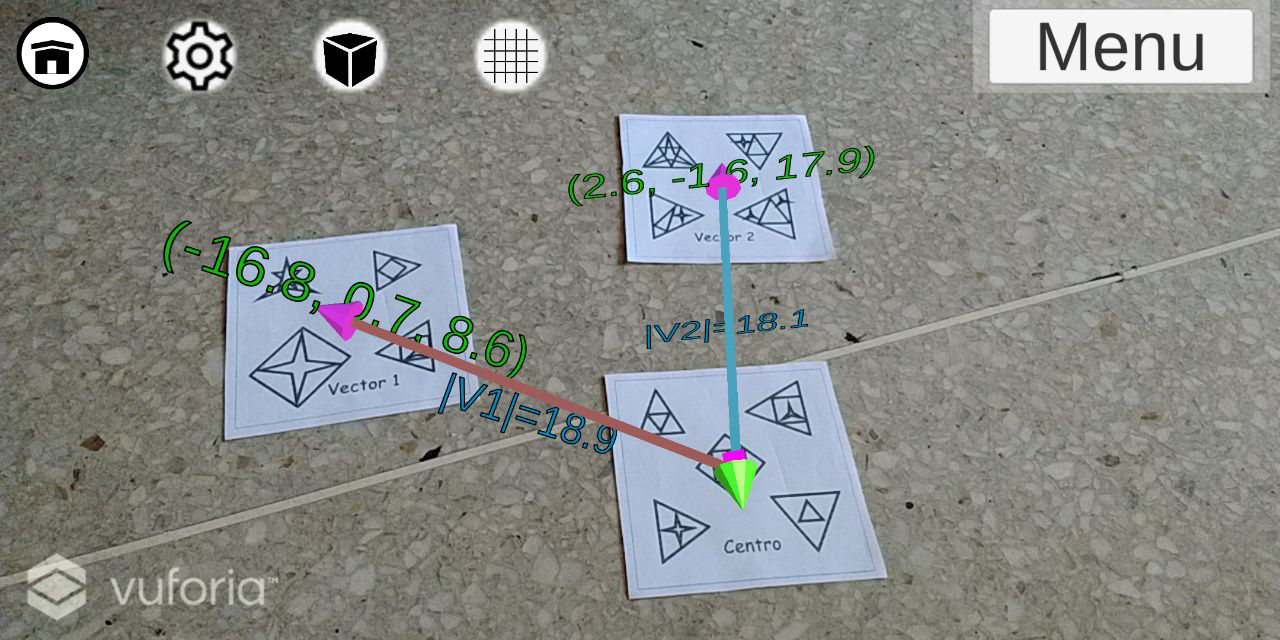
\includegraphics[width=0.5\textwidth]{figuras/vectores/Vectores1.png}
\caption{\label{fig:vec_ej1}Ejemplo de la aplicación de Vectores.}
\end{figure}
\FloatBarrier

\subsection{Image Render Target de Vuforia}
Para poder utilizar el motor de realidad aumentada de Vuforia, se generan tres \textit{Image Render Target}. Estos fueron utilizados como el centro donde comenzará cada uno de los vectores y los destinos del primer y segundo vector para controlar sus coordenadas. Para facilitar el reconocimiento por parte de Vuforia y minimizar las veces que los usuarios tengan que volver a apuntar las marcas con la cámara, se utilizaron figuras geométricas sencillas que apuntan en distintas direcciones con la finalidad de que el reconocedor de Vuforia tenga más información de la dirección de la imagen. 

En las Figuras \ref{fig:vec_centro} y \ref{fig:vec_vectores} se puede observar las marcas utilizadas, en estas se observa que se agregaron los nombres bajo ellas para facilitar su uso por los usuarios.

\begin{figure}[hbt!]
\centering
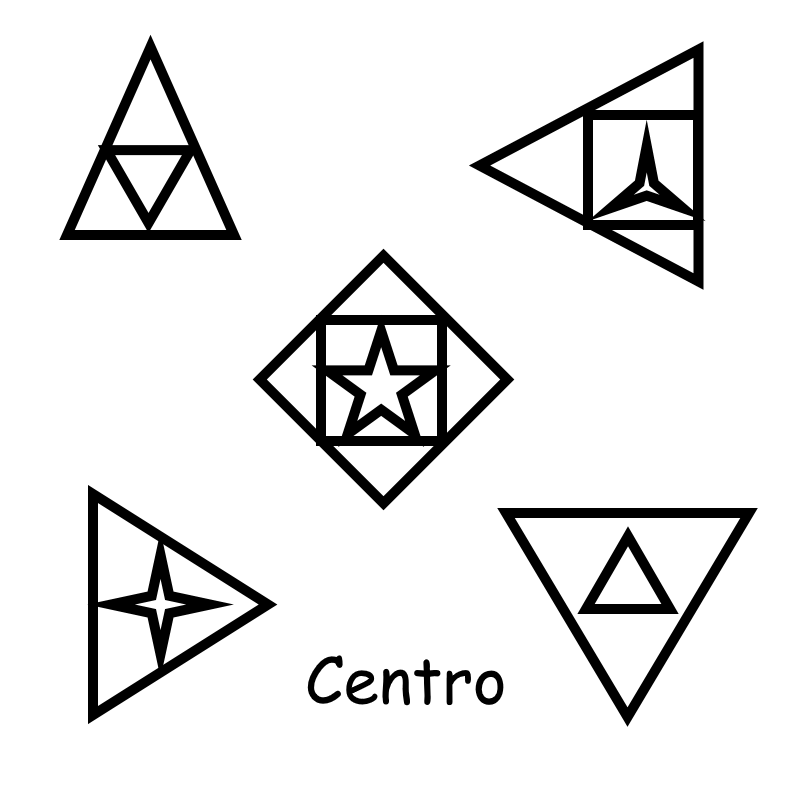
\includegraphics[width=0.5\textwidth]{figuras/vectores/ImageTarget1.png}
\caption{\label{fig:vec_centro}Marca de Centro para controlar el origen de los vectores.}
\end{figure}

\begin{figure}[hbt!]
\centering
\subfloat{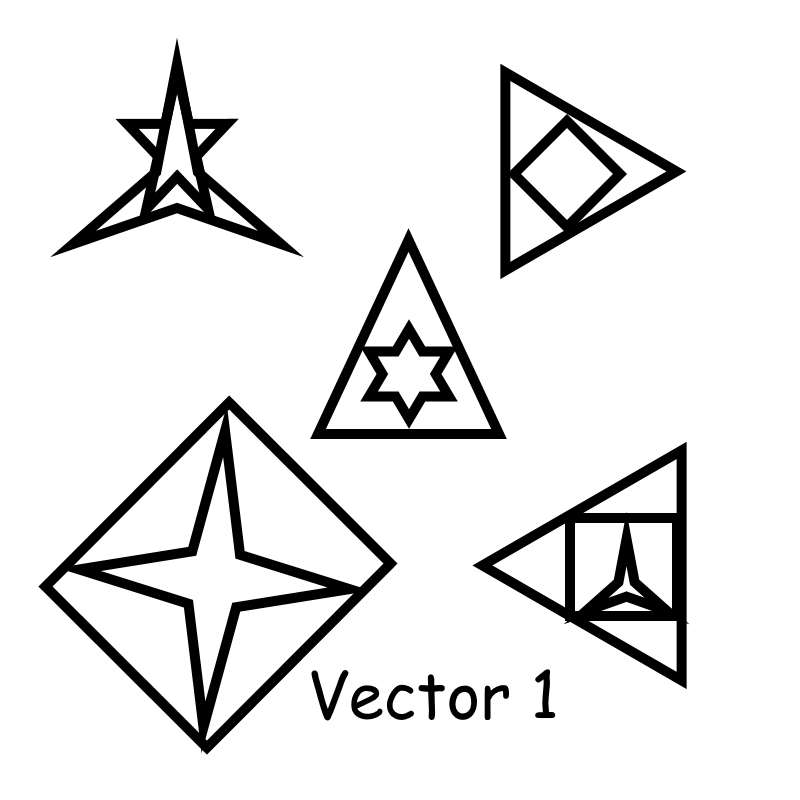
\includegraphics[width=0.5\textwidth]{figuras/vectores/ImageTarget2.png}}
\subfloat{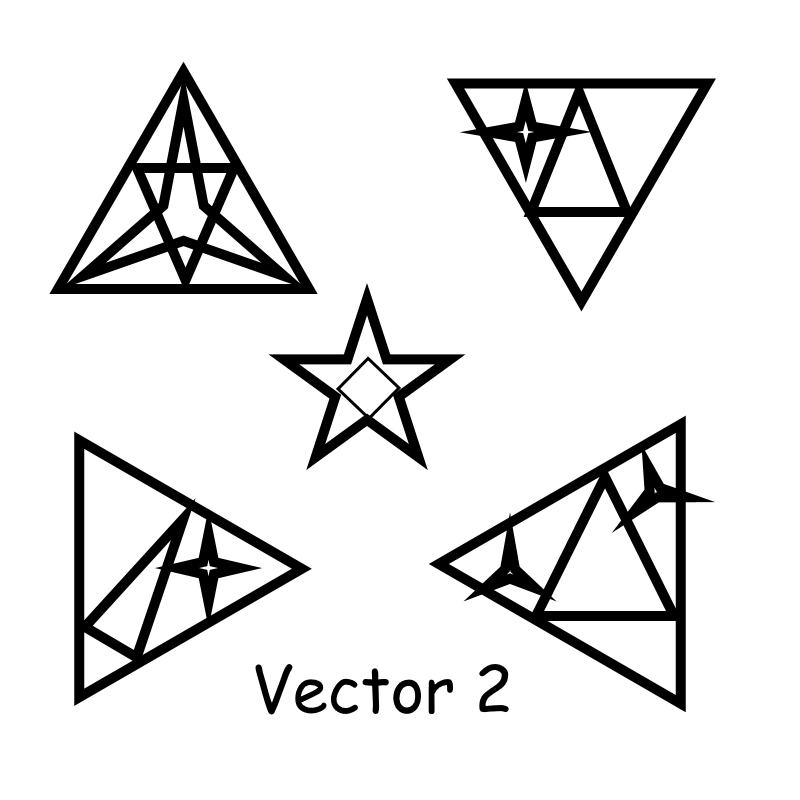
\includegraphics[width=0.5\textwidth]{figuras/vectores/ImageTarget3.png}}
\caption{\label{fig:vec_vectores}Marcas de Vector 1 y Vector 2 para controlar los destinos de los vectores.}
\end{figure}
\FloatBarrier

\subsection{Line Renderer}
Para representar los vectores gráficamente, se utilizó el componente \textit{Line Renderer} de Unity para el trazado de líneas y la simulación de los vectores a representar. Este componente es fácil de instanciar en la escena de la aplicación y de modificar, lo que permite que tanto los vectores, como los cálculos se realizan instantáneamente tanto al reconocer como al mover alguna de las marcas, lo que permite mayor agilidad y rapidez en el uso de la aplicación sin tener que esperar a que se vuelvan a calcular los datos. El principal problema que tiene este componente es que cada línea debe estar asociado a un \textit{GameObject} asociado, lo cual podría traer problemas de rendimiento si se instancian una gran cantidad de líneas en una escena. A pesar de esto, el proyecto no se vió afectado por esto ya que la mayor cantidad de líneas instanciadas a la vez, es igual a 16 (Figura \ref{fig:vec_linerenderer}), siendo la menor solo 2 al sólo representar los vectores.

\begin{figure}[hbt!]
\centering
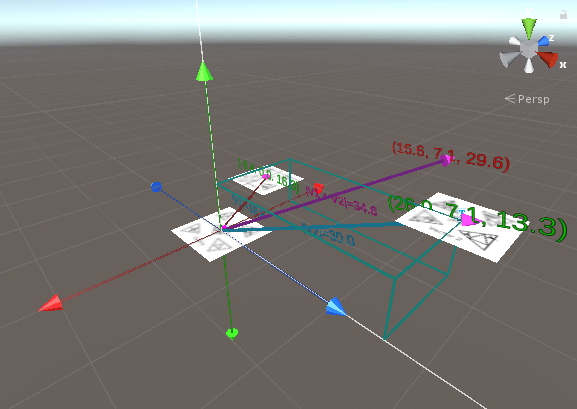
\includegraphics[width=0.5\textwidth]{figuras/vectores/LineRenderer.png}
\caption{\label{fig:vec_linerenderer}Escena de Unity con las opciones “Suma”, “Ejes Dobles” y “Proyección Vector 2” activadas, la cual en total suma 16 \textit{Line Renderers} instanciados.}
\end{figure}
\FloatBarrier

\subsection{Scripts} 
Los \textit{Scripts} se pueden dividir en tres grupos distintos, correspondiente a sus funcionalidades, implementación general de vectores, operaciones de vectores y componentes adicionales.

\subsubsection{Implementación General de Vectores} 

\paragraph{Representación de Vectores}
Cada vector viene representado en la aplicación por dos \textit{GameObjects}, el primero que contiene un \textit{Line Renderer} para poder renderizar la longitud del vector, y el segundo que contiene el modelo de flecha que está en el destino de cada vector y representa la dirección del mismo. Ambos son controlados por el \textit{script} \textit{AnimateLine.cs} el cual se encarga de cada vector independientemente de revisar primero si las marcas de Centro y Vector están detectadas, y en ese caso instanciar la línea y flecha dirigidas hacia la marca destino (Figura \ref{fig:vec_representacion}).

\begin{figure}[hbt!]
\centering
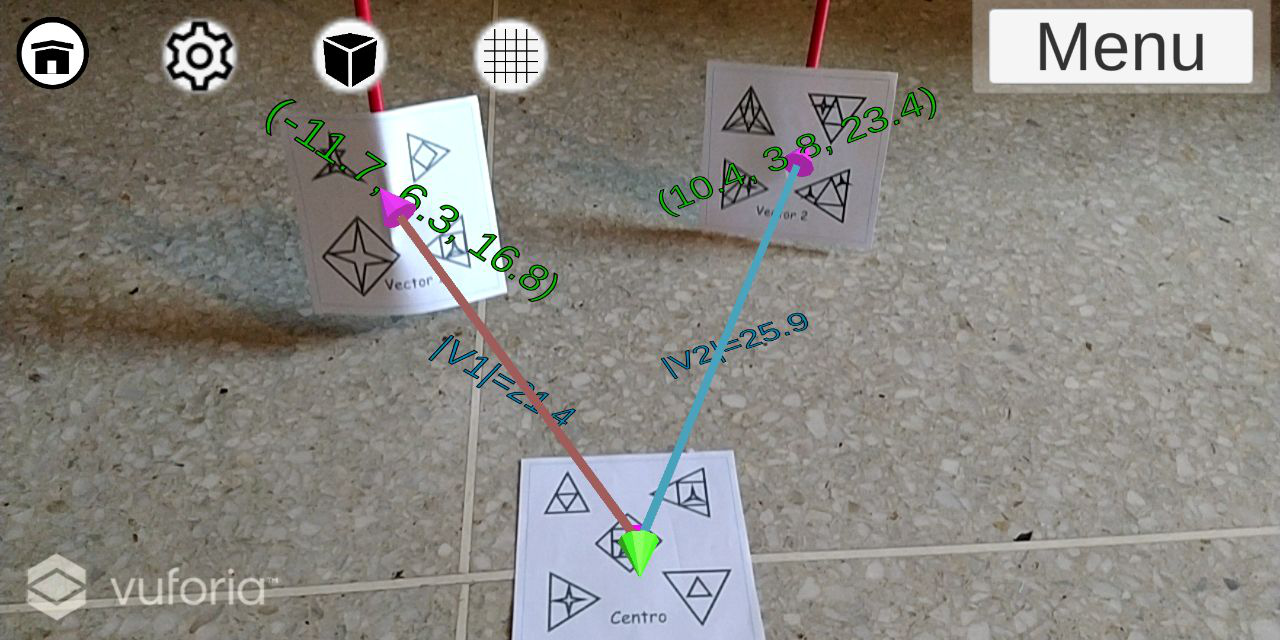
\includegraphics[width=0.5\textwidth]{figuras/vectores/RepresentacionVectores.png}
\caption{\label{fig:vec_representacion}Representación de vectores con sus marcas en la aplicación.}
\end{figure}

Una vez ya instanciado el vector en la aplicación, si se detecta algún movimiento en la marca (se revisa en cada frame si se detectó o no un movimiento) se actualizará automáticamente la longitud y dirección del vector, afectando también los cálculos mostrados en la interfaz gráfica.
\FloatBarrier

\paragraph{Tracker}
El \textit{Tracker} (o rastreador) se encarga de conectar las ejecuciones necesarias en la representación de vectores con el reconocedor de marcas de Vuforia. Específicamente, el \textit{script} \textit{Tracker.cs} llama a las distintas funciones de los otros scripts. Al reconocer Centro con Vector 1, se encarga de llamar a la función de representación de vector, y de igual manera al reconocer Centro con Vector 2. Al reconocer las tres marcas a la vez, llama a las funciones de operaciones que pueden estar activadas para poder representarlas en la aplicación.

\paragraph{Interfaz Gráfica (Componentes X,Y,Z y Módulo del Vector)}
El manejo de la interfaz gráfica se divide en cuatro \textit{scripts}, los cuales son: \textit{TextDistance.cs}, el cual está encargado de colocar el texto de la distancia entre los vectores y el centro, además de las posiciones en el espacio de ambos vectores; \textit{PlaneHandler.cs}, el cual se encarga de activar y desactivar los planos de los ejes de forma rotativa; \textit{SettingsHandler.cs}, que se encarga de cambiar el modo de renderizar los ejes de forma rotativa entre no eje, completo con parte negativa, normales y doblemente largos; finalmente está \textit{BoxHandler.cs}, el cual maneja el renderizado una caja construida por las proyecciones del vector contra los ejes y rota entre renderizarlo para uno de los vectores.

\subsubsection{Operaciones de vectores}
Una vez detectada las marcas, el usuario podrá hacer uso del cálculo de las operaciones de vectores al presionar el botón “Menu”, las cuales se dividen en suma, resta, producto cruz, producto punto y limpiar. Todos los cálculos de las operaciones se realizan en el script Functions.cs el cual contiene las fórmulas necesarias para calcular cada una de ellas y mostrar gráficamente el resultado con el vector resultante (compuesto por su longitud y dirección). Por último, solo se puede mostrar una operación a la vez.

\paragraph{Suma}
La operación de suma entre los vectores $u=(u_x,u_y,u_z)$ y $v=(v_x,v_y,v_z)$ en un plano de tres dimensiones viene representada por la fórmula $u + v = (u_x+v_x, u_y+v_y, u_z+v_z)$.

En la siguiente figura (Figura \ref{fig:vec_suma}) se muestra un ejemplo de la operación sumar en funcionamiento.

\begin{figure}[hbt!]
\centering
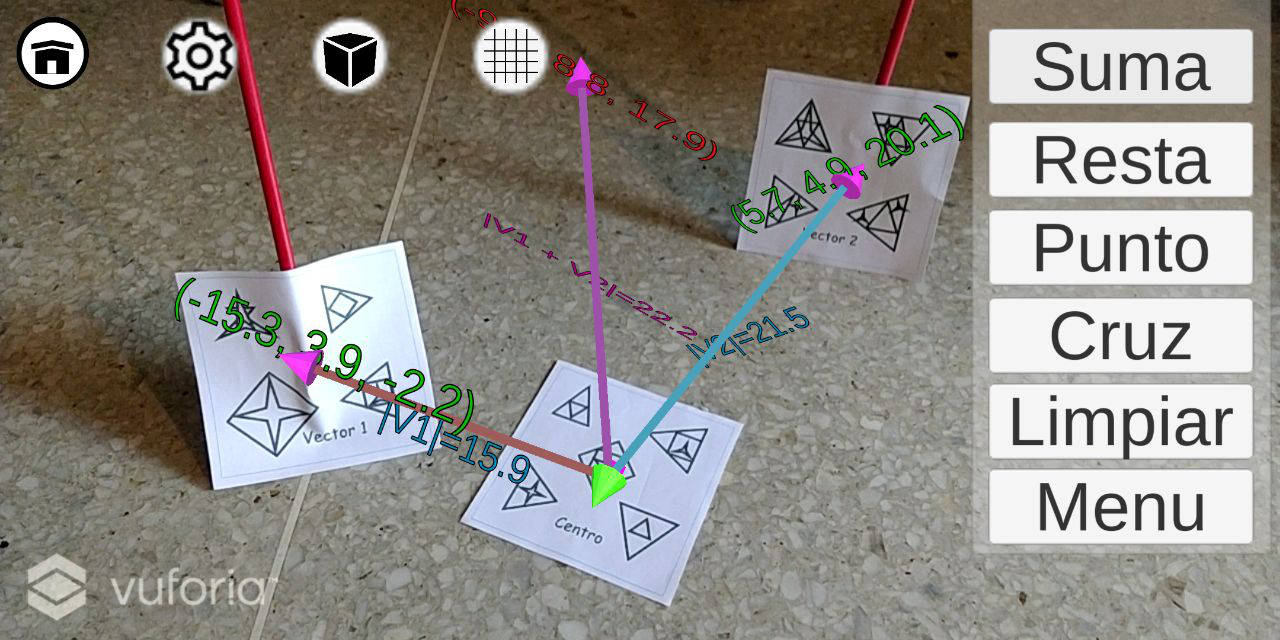
\includegraphics[width=0.5\textwidth]{figuras/vectores/Suma.png}
\caption{\label{fig:vec_suma}Operación sumar en la aplicación.}
\end{figure}
\FloatBarrier

\paragraph{Resta}
La operación de resta entre los vectores $u=(u_x,u_y,u_z)$ y $v=(v_x,v_y,v_z)$ en un plano de tres dimensiones viene representada por la fórmula $u - v = (u_x-v_x, u_y-v_y, u_z-v_z)$.

En la siguiente figura (Figura \ref{fig:vec_resta}) se muestra un ejemplo de la operación restar en funcionamiento.

\begin{figure}[hbt!]
\centering
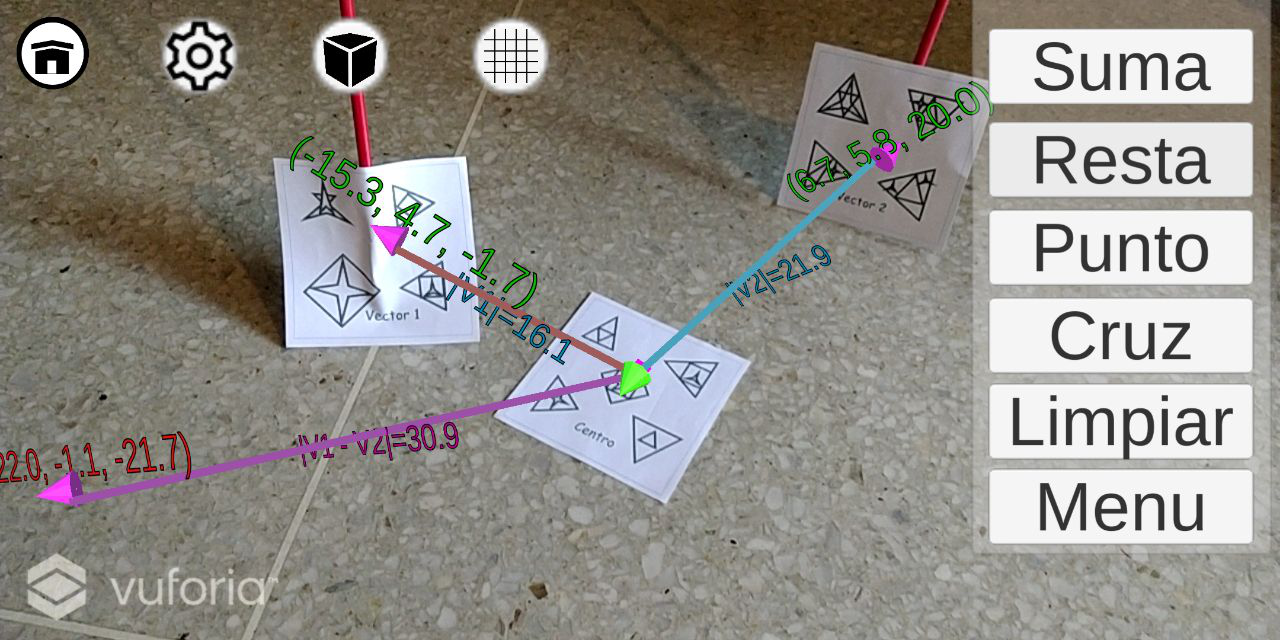
\includegraphics[width=0.5\textwidth]{figuras/vectores/Resta.png}
\caption{\label{fig:vec_resta}Operación restar en la aplicación.}
\end{figure}
\FloatBarrier

\paragraph{Producto Punto}
La operación de producto punto entre los vectores $u=(u_x,u_y,u_z)$ y $v=(v_x,v_y,v_z)$ en un plano de tres dimensiones viene representada por la fórmula $u . v = | u | | v | cos(u,v)$, en donde $| u | = \sqrt{u_x^2 + u_y^2 + u_z^2}$.

En la siguiente figura (Figura \ref{fig:vec_punto}) se muestra un ejemplo de la operación producto punto en funcionamiento.

\begin{figure}[hbt!]
\centering
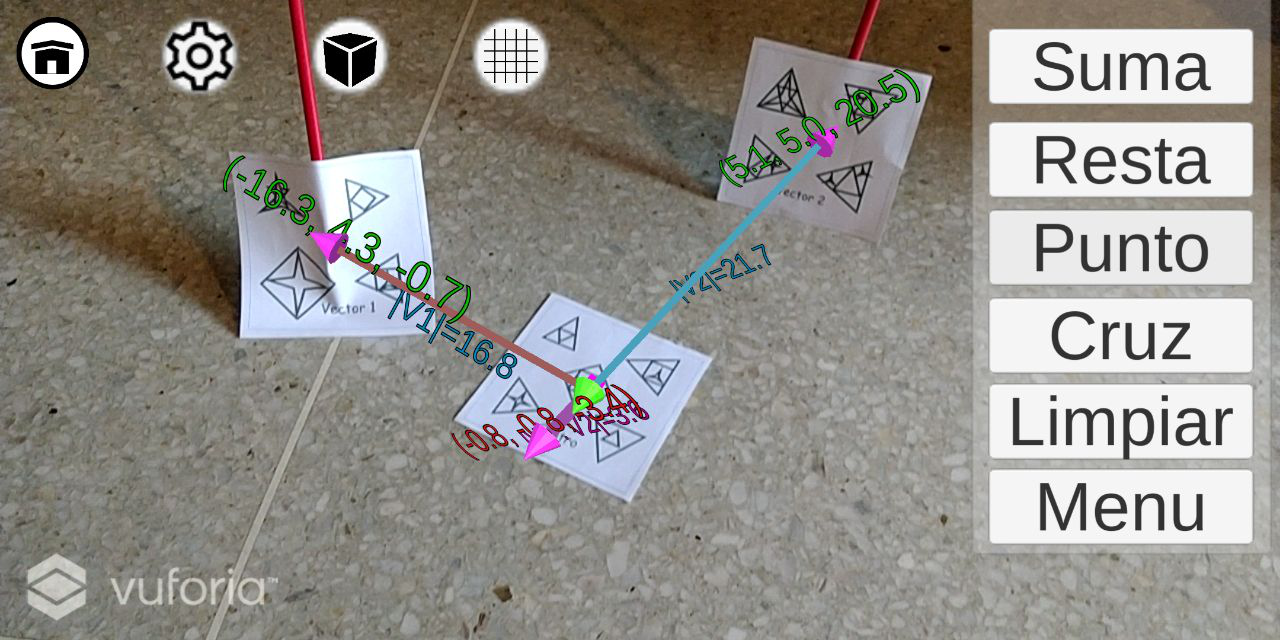
\includegraphics[width=0.5\textwidth]{figuras/vectores/ProductoPunto.png}
\caption{\label{fig:vec_punto}Operación producto punto en la aplicación.}
\end{figure}
\FloatBarrier

\paragraph{Producto Cruz}
La operación de producto cruz entre los vectores $u=(u_x,u_y,u_z)$ y $v=(v_x,v_y,v_z)$ en un plano de tres dimensiones viene representada por la fórmula $u \times v = (u_y*v_z - u_z*v_y, u_z*v_x - u_x*v_z, u_x*v_y - v_y*v_x)$.

En la siguiente figura (Figura \ref{fig:vec_cruz}) se muestra un ejemplo de la operación producto cruz en funcionamiento.

\begin{figure}[hbt!]
\centering
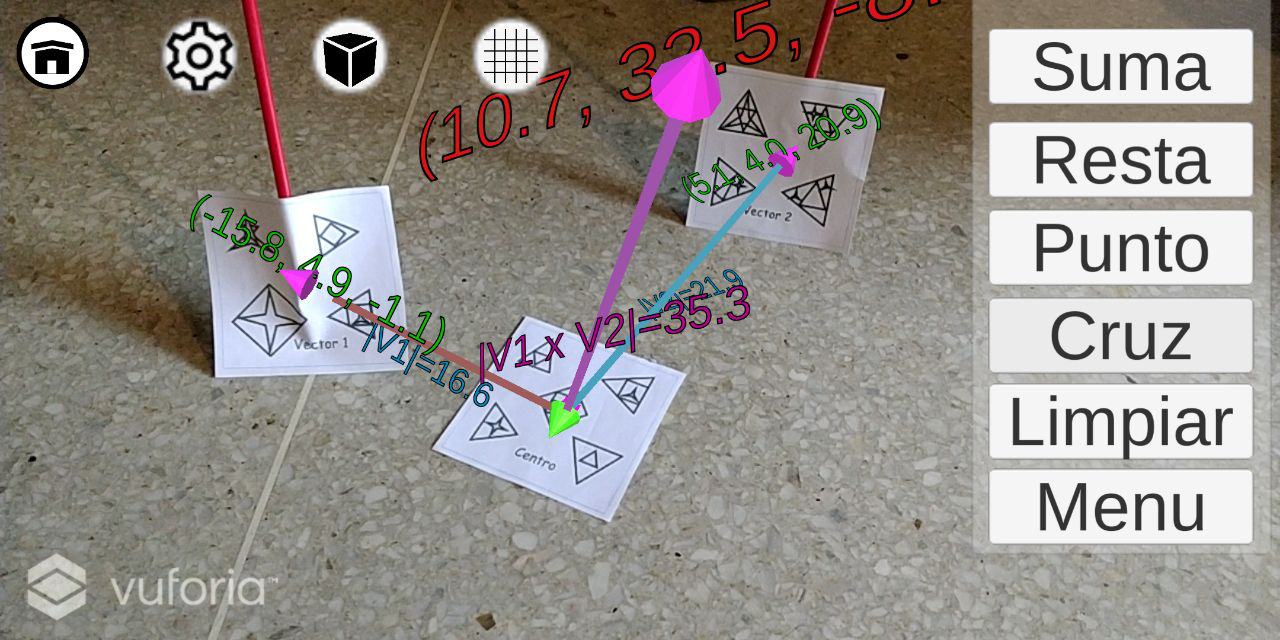
\includegraphics[width=0.5\textwidth]{figuras/vectores/ProductoCruz.png}
\caption{\label{fig:vec_cruz}Operación producto cruz en la aplicación.}
\end{figure}
\FloatBarrier

\paragraph{Limpiar}

La operación Limpiar se encarga de desactivar la función previamente activada y mostrar únicamente la interfaz original con la representación de los dos vectores.

\subsubsection{Componentes adicionales}
Por último, aparte de las operaciones de vectores en la interfaz gráfica, se encuentran cuatro botones: volver al menú principal, cambiar ejes, proyección de vectores y planos en el origen. Estas opciones se pueden activar independientes a las operaciones, es decir, no tienen restricciones entre ellas y se pueden ver todas activadas al mismo tiempo.

\paragraph{Ejes del origen}
El botón de ejes en el origen, permite al usuario colocar distintos tipos de ejes en las coordenadas $(x,y,z)$ para facilitar la visualización del plano cartesiano. Estas operaciones son calculadas en el \textit{script} \textit{AnimateLineAxis.cs} que se encarga únicamente de instanciar cada uno de los ejes con su dirección determinada.  Las distintas opciones que se encuentran son:

\begin{enumerate}
    \item Desactivado.
    \item Ejes positivos.
    \item Ejes positivos y negativos (Figura \ref{fig:vec_opcion_ejes}).
    \item Ejes positivos extendidos.
\end{enumerate}

\begin{figure}[hbt!]
\centering
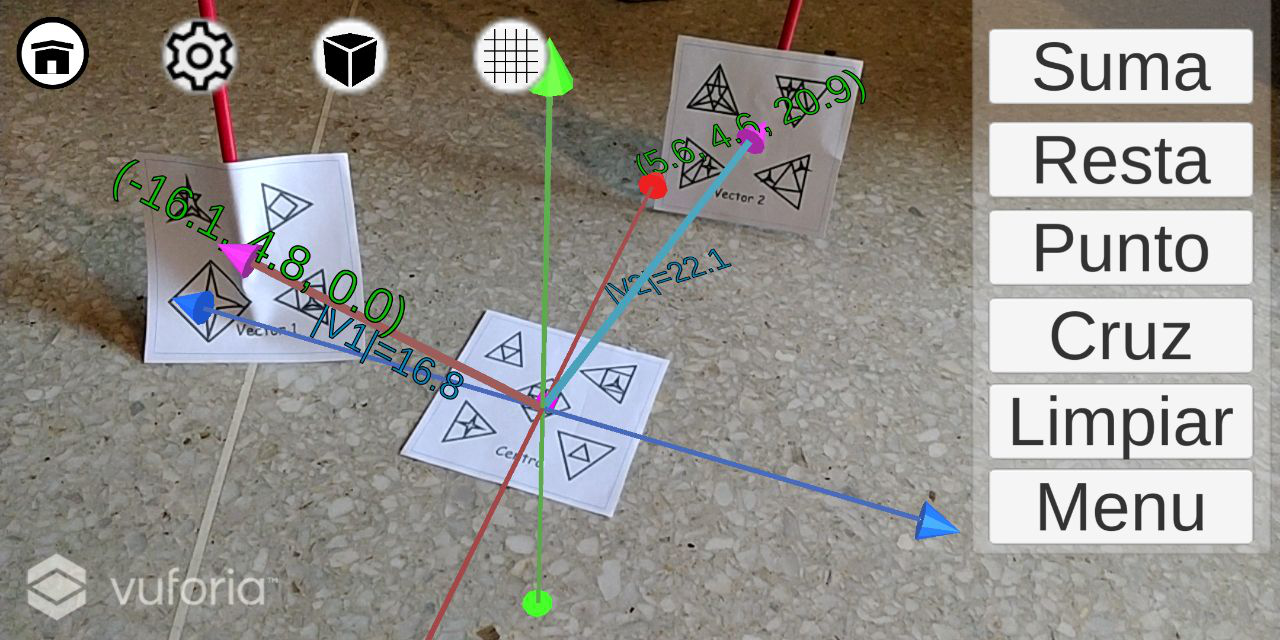
\includegraphics[width=0.5\textwidth]{figuras/vectores/Ejes.png}
\caption{\label{fig:vec_opcion_ejes}Opción de ejes positivos y negativos activada en la aplicación.}
\end{figure}
\FloatBarrier

\paragraph{Proyección del Vector}
El botón de proyección de vectores permite representar la proyección de uno de los dos vectores de acuerdo a su origen y destino. Dependiendo de cuál vector se encuentre activado, además cambia el color del botón (verde para Vector 1 y azul para Vector 2). Estas operaciones se realizan en el \textit{script} \textit{AnimateAxis.cs} asociado a cada vector, y se encarga de instanciar cada una de las líneas para finalmente proyectar el vector, representado en el plano de tres dimensiones como un cubo. Las distintas opciones que se encuentran son:

\begin{enumerate}
    \item Desactivado.
    \item Proyección del Vector 1 (Figura \ref{fig:vec_opcion_proyeccion}).
    \item Proyección del Vector 2.
\end{enumerate}

\begin{figure}[hbt!]
\centering
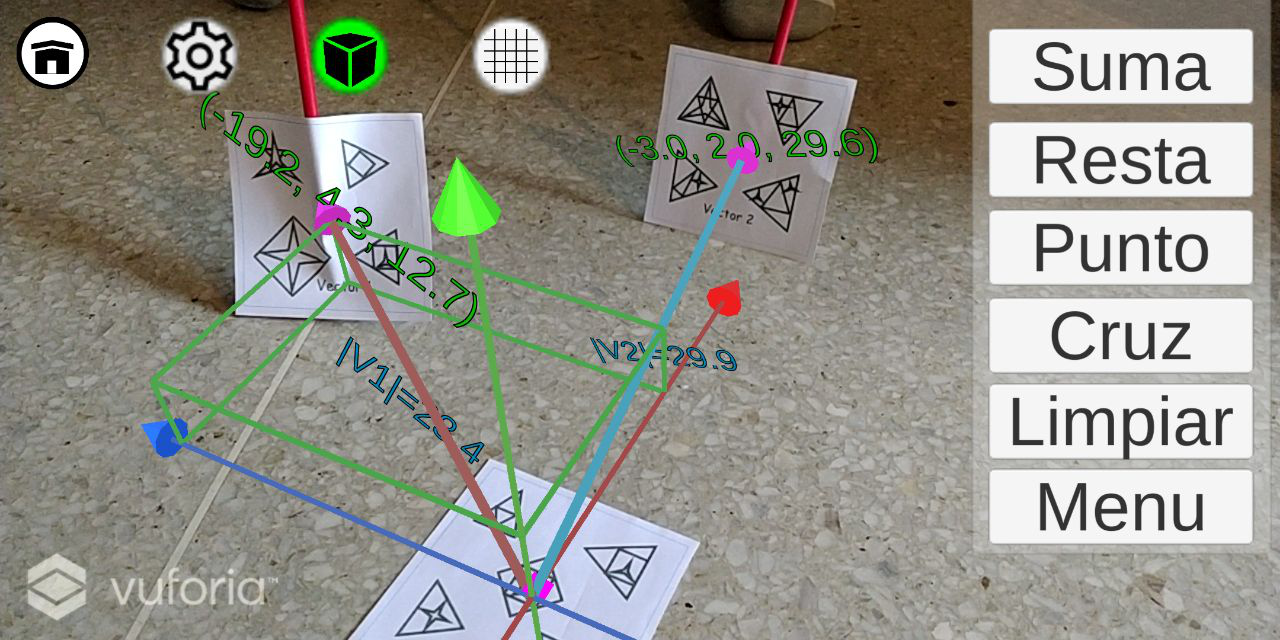
\includegraphics[width=0.5\textwidth]{figuras/vectores/Proyeccion.png}
\caption{\label{fig:vec_opcion_proyeccion}Opción de proyección del Vector 1 activada.}
\end{figure}
\FloatBarrier

\paragraph{Planos en el Origen}
El botón de planos en el origen permite al usuario instanciar en la escena un plano cartesiano que facilita las mediciones de los vectores. Cada plano tiene una medida de $30\times 30$ cuadrículas, cada una de aproximadamente $1\times 1cm$ reales. Estos planos se instancian en el \textit{script} \textit{AnimateLineAxis.cs}. Las distintas opciones que se encuentran disponibles son:

\begin{enumerate}
    \item Desactivado.
    \item Plano en el eje x (Figura \ref{fig:vec_opcion_planos_x}).
    \item Plano en el eje y.
    \item Plano en el eje z.
    \item Planos en los ejes x,y,z (Figura \ref{fig:vec_opcion_planos_xyz}).
\end{enumerate}

\begin{figure}[hbt!]
\centering
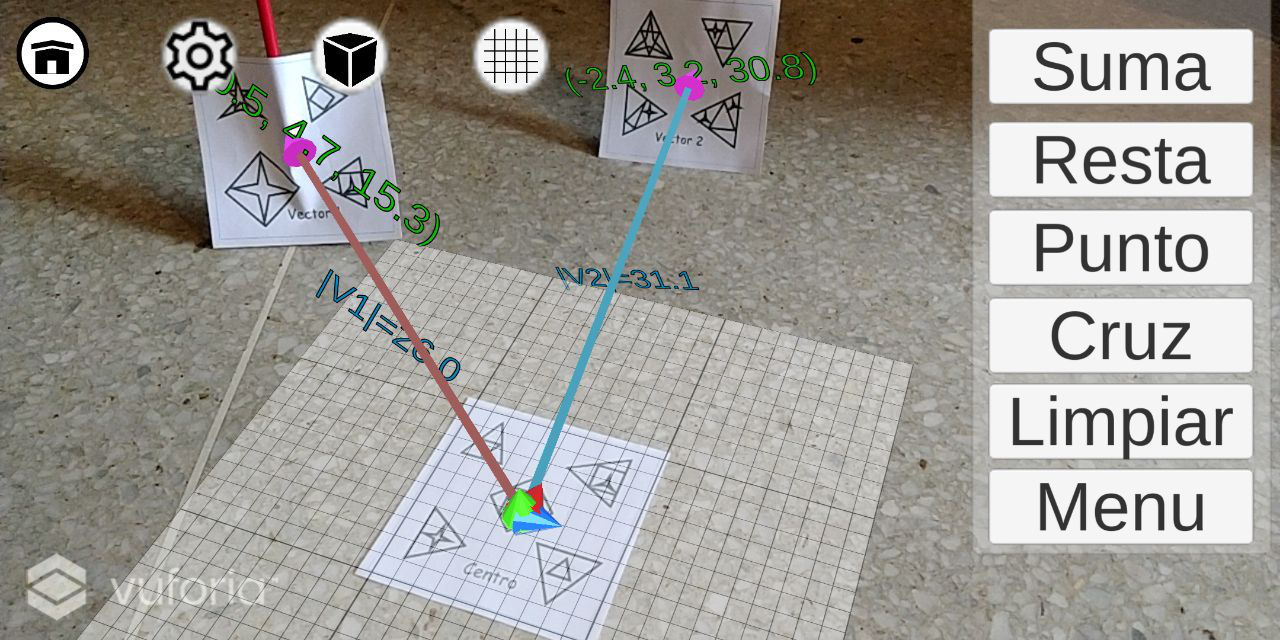
\includegraphics[width=0.5\textwidth]{figuras/vectores/Planos1.png}
\caption{\label{fig:vec_opcion_planos_x}Opción de plano en el eje x activada.}
\end{figure}

\begin{figure}[hbt!]
\centering
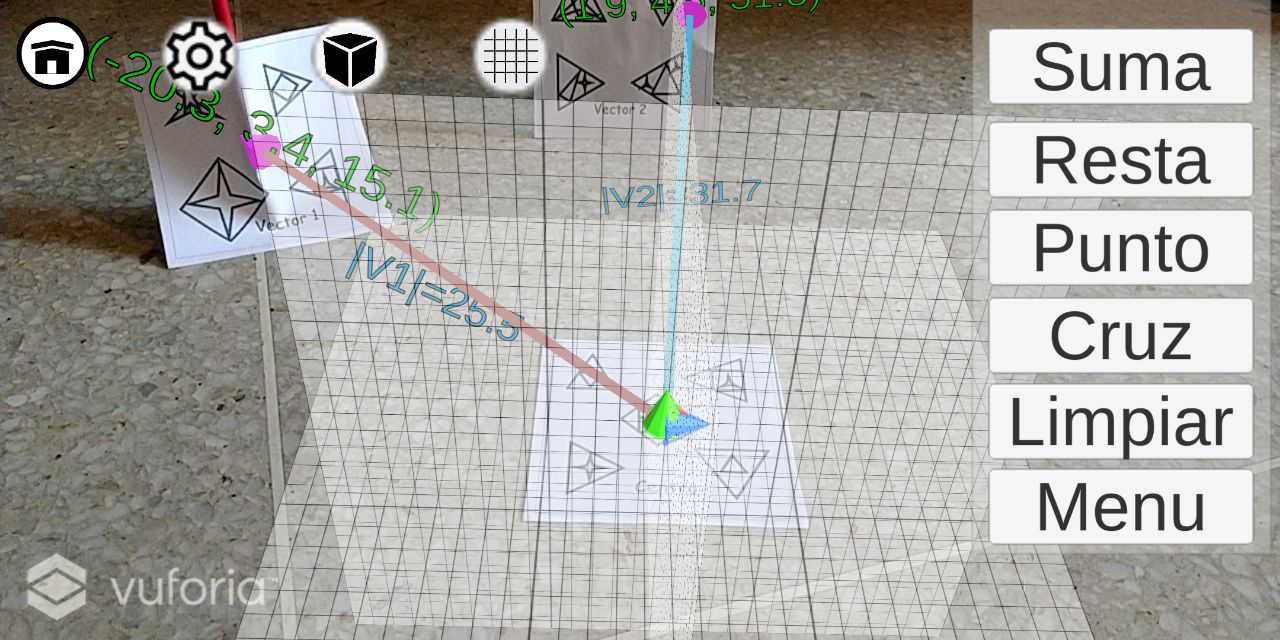
\includegraphics[width=0.5\textwidth]{figuras/vectores/Planos2.png}
\caption{\label{fig:vec_opcion_planos_xyz}Opción de planos en los ejes x,y,z activada.}
\end{figure}
\FloatBarrier

\subsection{Consideraciones Importantes al Momento de Realizar Operaciones} 
En el editor de escenas de Unity, las unidades al momento de ser calculadas están definidas en Unidades de Vuforia, a diferencia de una unidad utilizada en la vida real como centímetros o pulgadas. Uno de los retos del proyecto fue encontrar cual era la relación entre unidades de Vuforia y centímetros para que los vectores tengan las mismas mediciones al ser utilizadas por la aplicación en la vida real. Luego de realizar varias pruebas, se encontró que utilizando marcas de detección de $10\times 10cm$, se encuentra que la relación entre unidades de Vuforia y centímetros es de $1:1$, es decir son totalmente equivalentes. Esto permite que la representación de los vectores tengan a lo sumo un margen de error de $1 cm$ al momento de ser calculados por Vuforia y la aplicación.


\section{VisualizAR: Gráficas}
Esta sección de la aplicación se busca presentar los conceptos de gráficas a estudiantes de bachillerato, mediante la presentación interactiva de distintas funciones parametrizables con dos coordenadas, las cuales son manifestadas en 3D mediante el uso de la realidad aumentada. Además, se utiliza al tiempo como un tercer parámetro, para aumentar el llamativo de las gráficas. En las Figuras \ref{fig:graf_ej1}, \ref{fig:graf_ej2} y \ref{fig:graf_ej3} se pueden observar ejemplos de esta aplicación.

Para realizar esto se utilizaron dos \textit{Image Render Target} de Vuforia, uno como base y otro como menú; un \textit{Shader} para la coloración de la gráfica y cuatro \textit{Scripts} de control.

\begin{figure}[hbt!]
\centering
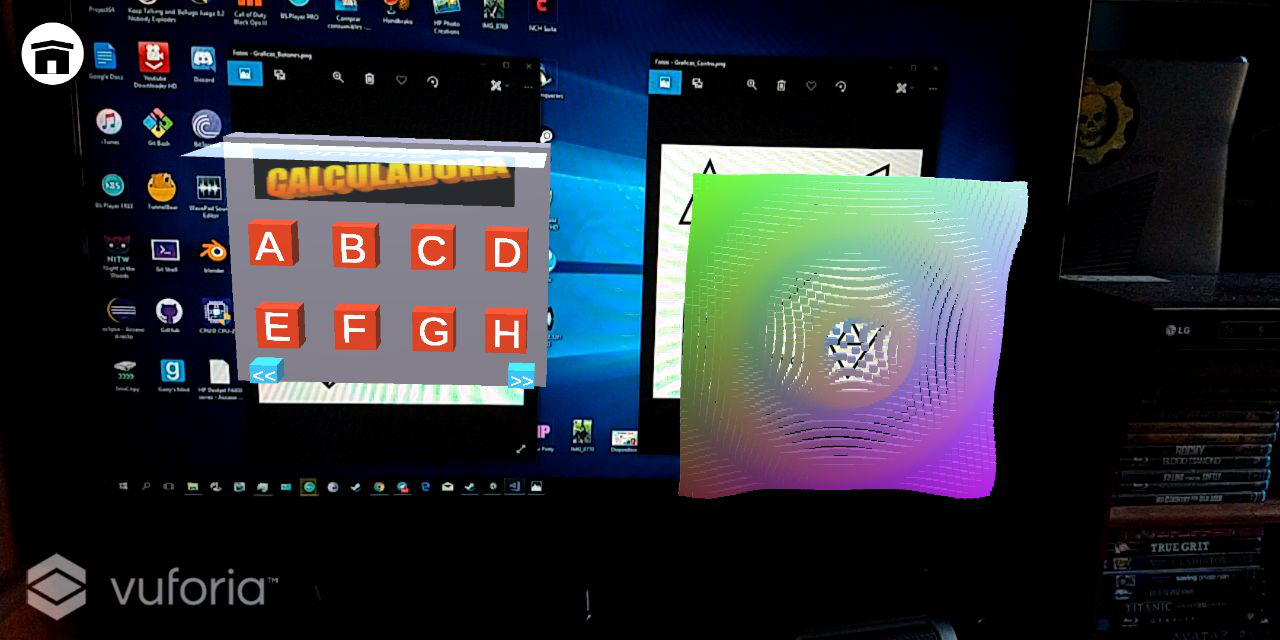
\includegraphics[width=0.5\textwidth]{figuras/graficas/ej1.png}
\caption{\label{fig:graf_ej1}Ejemplo de la aplicación de Gráficas.}
\end{figure}

\begin{figure}[hbt!]
\centering
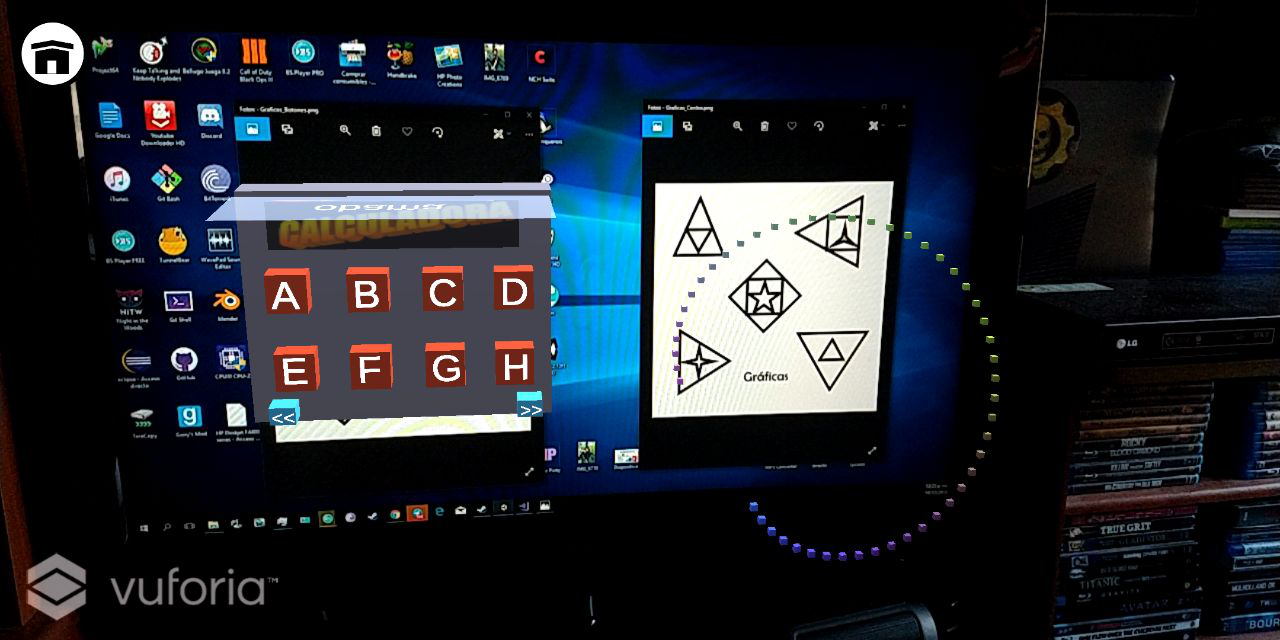
\includegraphics[width=0.5\textwidth]{figuras/graficas/ej2.png}
\caption{\label{fig:graf_ej2}Ejemplo de la aplicación de Gráficas.}
\end{figure}

\begin{figure}[hbt!]
\centering
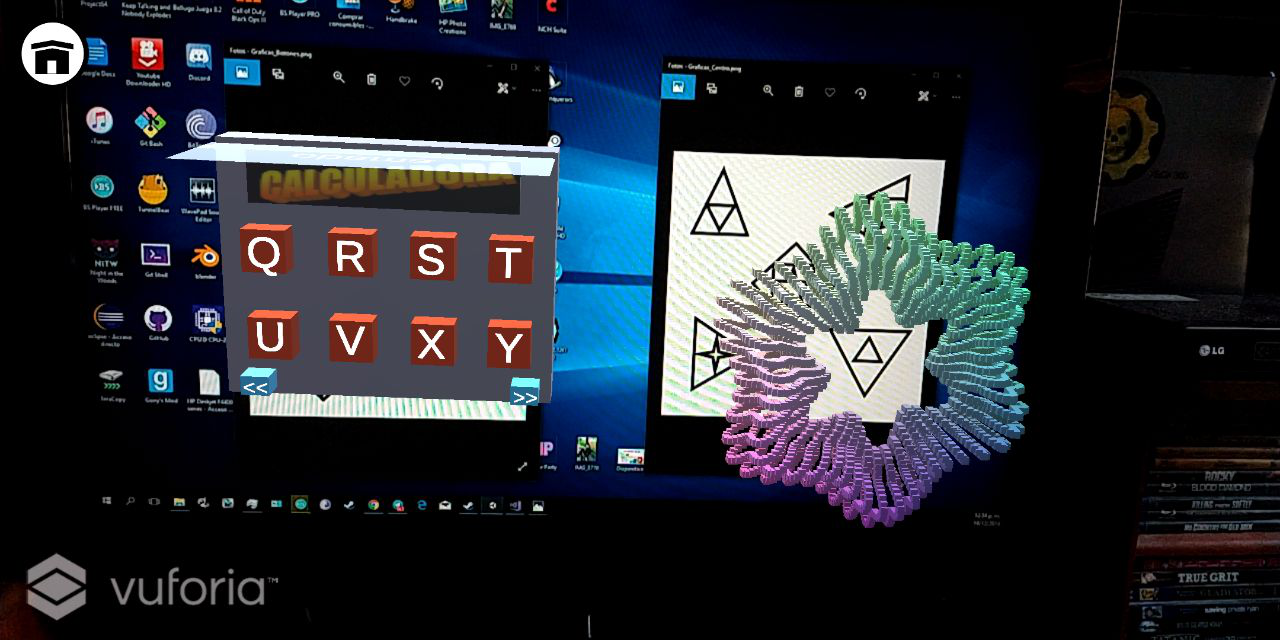
\includegraphics[width=0.5\textwidth]{figuras/graficas/ej3.png}
\caption{\label{fig:graf_ej3}Ejemplo de la aplicación de Gráficas.}
\end{figure}
\FloatBarrier

\subsection{Image Render Target de Vuforia}
Para poder utilizar el motor de realidad aumentada de Vuforia, se generaron dos \textit{Image Render Target}. Estos fueron utilizados como la base donde poder mostrar las gráficas y los botones para controlar la selección de qué función visualizar.

En las Figuras \ref{fig:graf_botones} y \ref{fig:graf_centro} se puede observar las marcas utilizadas, en estas se observa que se agregaron los nombres bajo ellas para facilitar su uso por los usuarios.

\begin{figure}[hbt!]
\centering
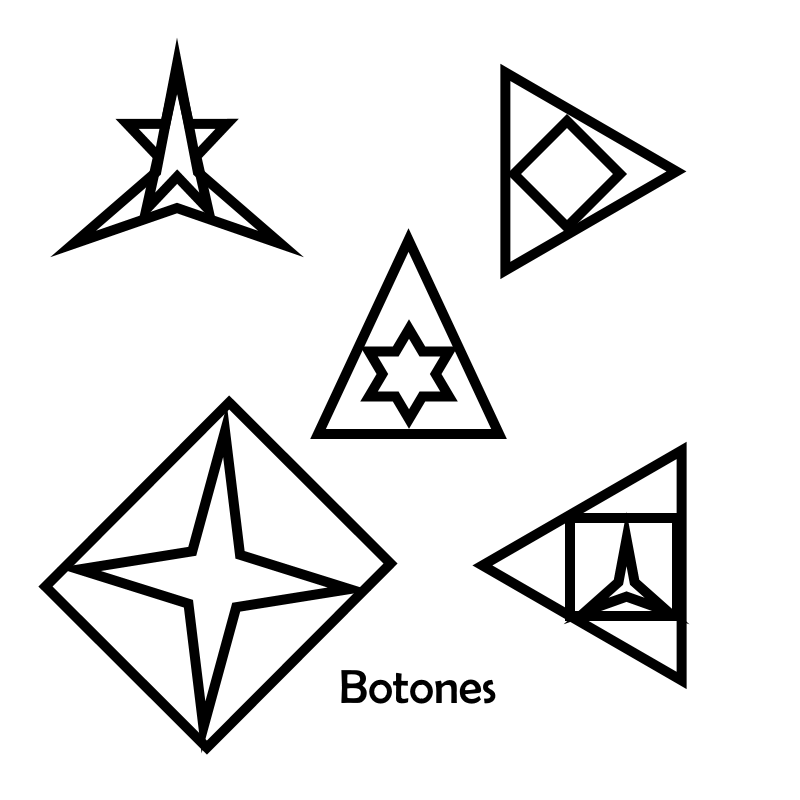
\includegraphics[width=0.4\textwidth]{figuras/graficas/botones.png}
\caption{\label{fig:graf_botones}Marca de Botones para controlar la aplicación.}
\end{figure}

\begin{figure}[hbt!]
\centering
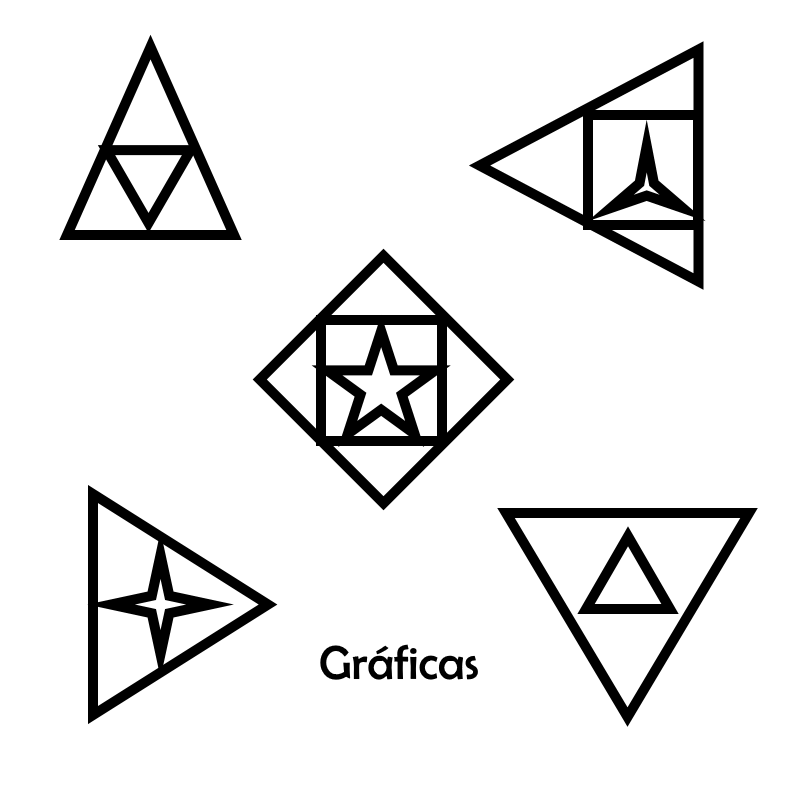
\includegraphics[width=0.4\textwidth]{figuras/graficas/centro.png}
\caption{\label{fig:graf_centro}Marca de Gráficas para controlar la posición donde visualizar las funciones.}
\end{figure}
\FloatBarrier

\subsection{Shader}
Para aumentar el llamativo visual de las gráficas, se creó un \textit{Shader} para controlar la forma de colorear. Este se basa en mostrar la representación del espacio vectorial, centrado en base, en el espacio de colores RGB. Esto se realiza mediante la normalización del espacio, utilizando un factor de escalamiento, para pasar al espacio $[-1,1]\times[-1,1]\times[-1,1]$ y luego transformarlo al espacio $[0,1]\times[0,1]\times[0,1]$, el cual es representable como un color RGB. El código se puede encontrar en la carpeta de \textit{Shaders} bajo el nombre \textit{ColoredPoint.shader}. En la Figura \ref{fig:graf_shader} se observa un ejemplo de la coloración generada por el \textit{Shader}.

\begin{figure}[hbt!]
\centering
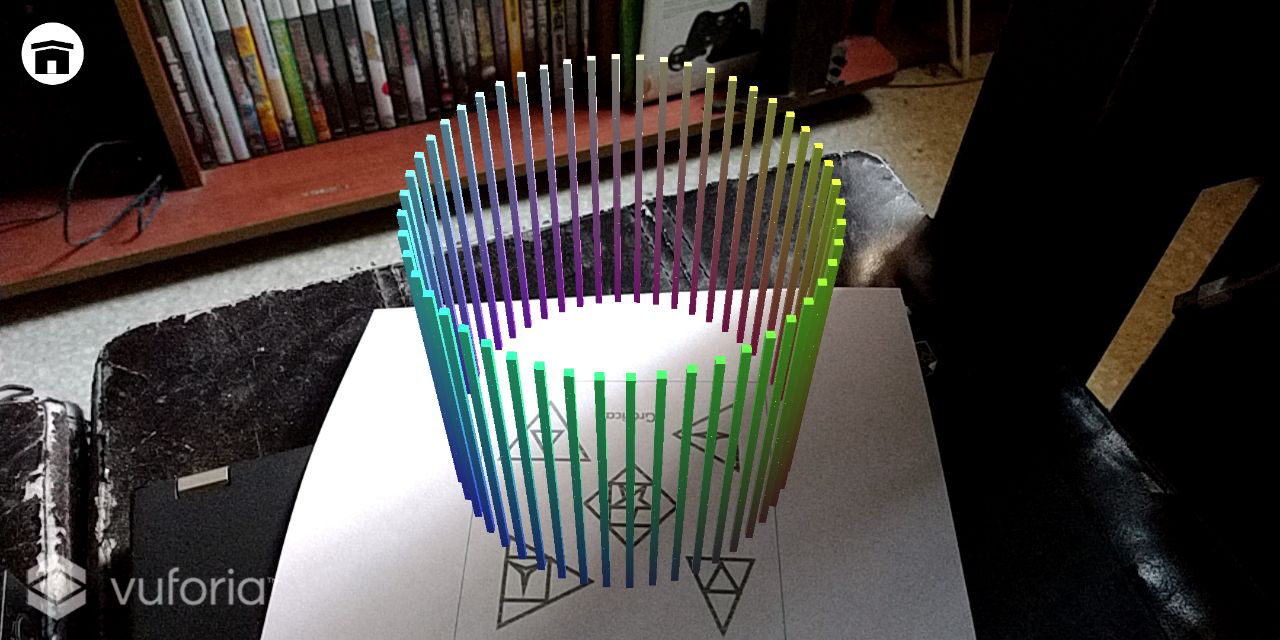
\includegraphics[width=0.5\textwidth]{figuras/graficas/shader.png}
\caption{\label{fig:graf_shader}Ejemplo de la visualización del espacio vectorial mediante colores RGB.}
\end{figure}
\FloatBarrier

\subsection{Scripts}
Los \textit{Scripts} se pueden dividir en dos grupos, los que manejan las gráficas y el que maneja la interfaz.

\subsubsection{Manejo de Gráficas} 
El proceso de graficar se realiza mediante la parametrización de superficies. En el caso de la aplicación, se parametrizan superficies 3D mediante coordenadas 2D del espacio $[0,1]\times[0,1]$, conocido en inglés como U V Mapping, el cual consiste en proyectar un plano 2D a una superficie 3D. Además, se incluye un parámetro de tiempo para darle un aspecto dinámico a las gráficas para atraer la atención del usuario. El desarrollo del manejador de gráficas se basó en las explicaciones de Jasper Flick \cite{flick2017}, adaptado a los requerimientos específicos de la aplicación y con más funciones.

Las funciones utilizadas en la aplicación para generar las superficies visualizadas tienen la forma presentada en la Ecuación \ref{eq:graf_func}, es importante destacar que no siempre tienen que usar los tres parámetros de entrada.

\begin{equation}\label{eq:graf_func}
\begin{aligned}
    & [0,1]\times[0,1]\times\mathbb{R}^+ \rightarrow \mathbb{R}^3 \\
    & f(u,v,t) = (x,y,z)
\end{aligned}
\end{equation}

Para representar los puntos de la superficie, se utilizó una malla 2D de $100 \times 100$ cubos (para darles un tamaño visible por los usuarios), la cual se instancia al comienzo de la aplicación de gráficas y  se adapta dinámicamente a la función que se desea graficar. Un ejemplo para visualizar los cubos que forman la superficie, es la gráfica del círculo de la Figura \ref{fig:graf_malla}. 

\begin{figure}[hbt!]
\centering
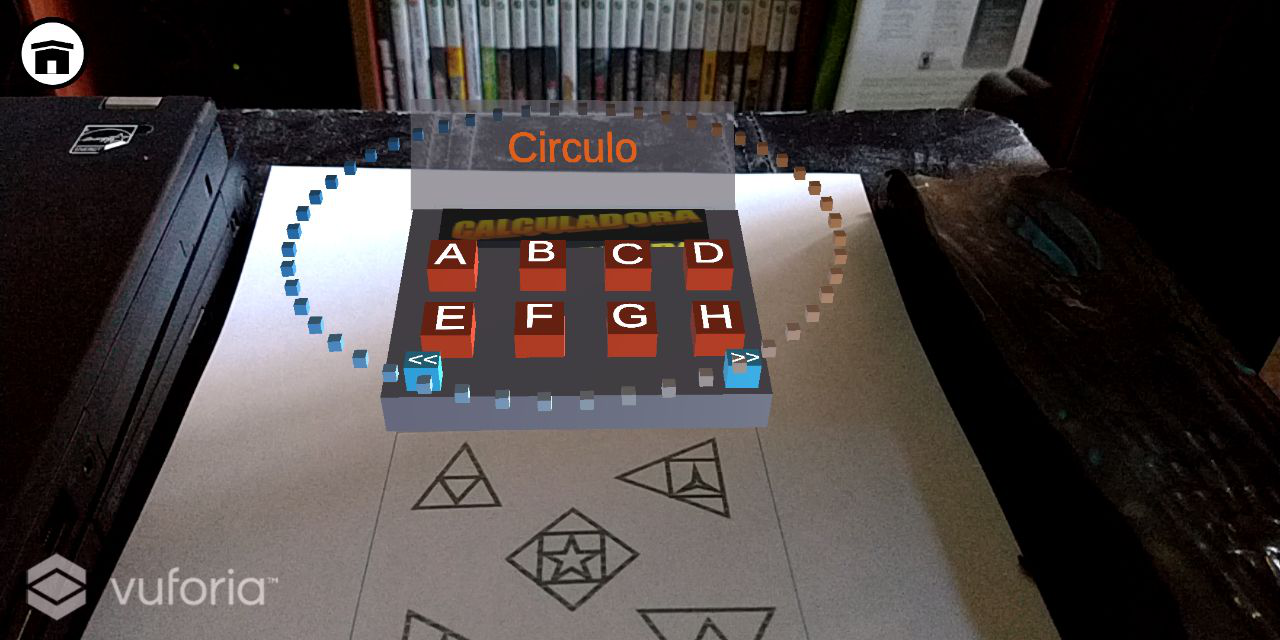
\includegraphics[width=0.5\textwidth]{figuras/graficas/malla.png}
\caption{\label{fig:graf_malla}Gráfica del círculo donde se observan los cubos que forman la malla.}
\end{figure}

Todo esto es manejado por el \textit{Script} \textit{Graph.cs}, el cual, además, controla las funciones para graficar. Para facilitar desarrollo y la futura posible expansión, se agregaron: \textit{GraphFunction.cs} el cual contiene el prototipo de las funciones que se grafican, para poder crear y utilizar más funciones; y \textit{GraphFunctionName.cs} el cual contiene un enumerable de los nombres de las funciones, para poder visualizarlas mejor en los menús dentro del editor de Unity.
\FloatBarrier

\subsubsection{Calculadora}
La calculadora se encarga de darle el control al usuario de decidir cuál gráfica mostrar al presionar cada uno de los botones sin necesidad de tener estas opciones en la interfaz gráfica. Por facilidad, se decidió tener tres páginas diferentes de opciones de ocho botones cada uno (identificados con una letra), las cuales pueden ser presionadas, emitiendo un sonido y animacion; e inmediatamente cambiar la gráfica actual. Aparte, la calculadora muestra una pequeña pantalla transparente la cual contiene el nombre de la gráfica actual. En la Figura \ref{fig:graf_calculadora} se puede observar la calculadora como se ve en la aplicación.

\begin{figure}[hbt!]
\centering
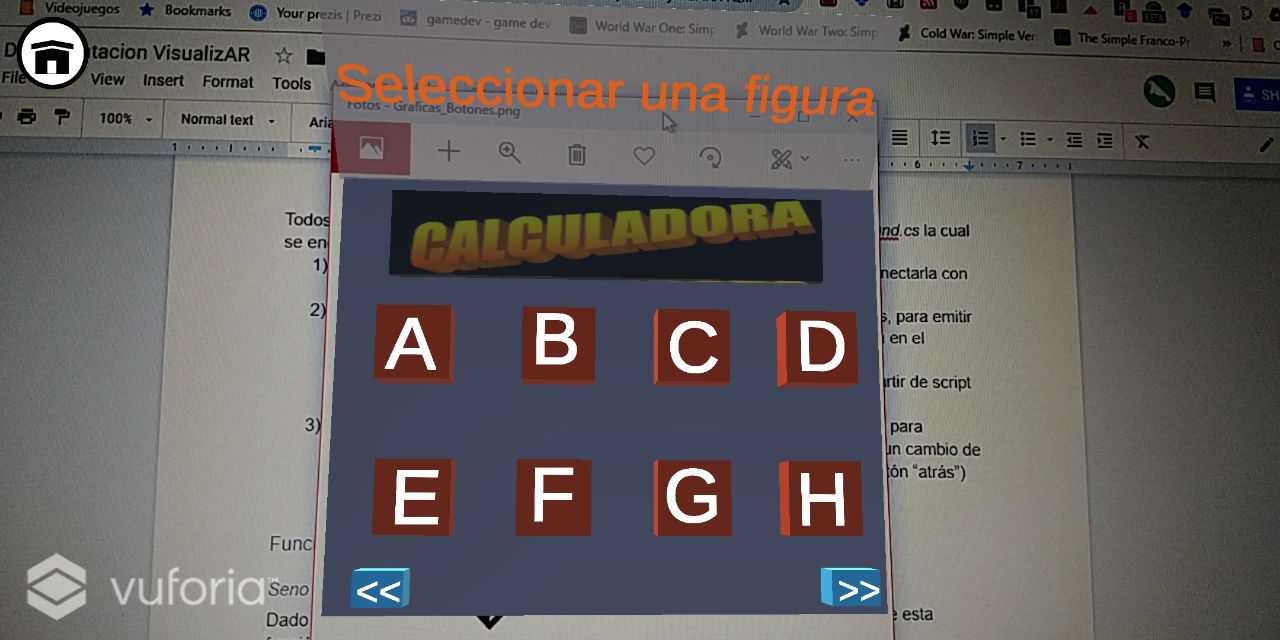
\includegraphics[width=0.5\textwidth]{figuras/graficas/calculadora.png}
\caption{\label{fig:graf_calculadora}Calculadora como se ve en la aplicación.}
\end{figure}

Todos los procedimientos y funciones de la calculadora están calculados en \textit{ARsound.cs} la cual se encarga de:
\begin{enumerate}
	\item Inicializar la calculadora con la primera página y primera función, Seno y conectarla con el Manejador de Funciones.
	\item Detectar cuando el usuario ha presionado alguno de los botones de gráficas, para emitir una animación de presionado de botón, un sonido y cambiar tanto la gráfica en el Manejador de Funciones como la pantalla de la calculadora con el nombre correspondiente. Cabe resaltar que la pequeña animación es realizada a partir de script y no con el animador de Unity.
	\item Detectar cuando el usuario ha presionado alguno de los cambios de página para actualizar la interfaz de la calculadora. En caso de que el usuario presione un cambio de página incorrecto (por ejemplo, estar en la primera página y presionar el botón “atrás”) se emite un sonido de error diferente al sonido predeterminado.
\end{enumerate}

\FloatBarrier

\subsubsection{Funciones} 
La aplicación consta de veinticuatro funciones para graficar, estas son explicadas a continuación.

\paragraph{Seno}
Dado por la ecuación $f(u,v,t)=(u,Sen(\pi * (u + t)),v)$. La Figura \ref{fig:graf_seno} es la gráfica de esta función, la cual es la opción A del menú.

\begin{figure}[hbt!]
\centering
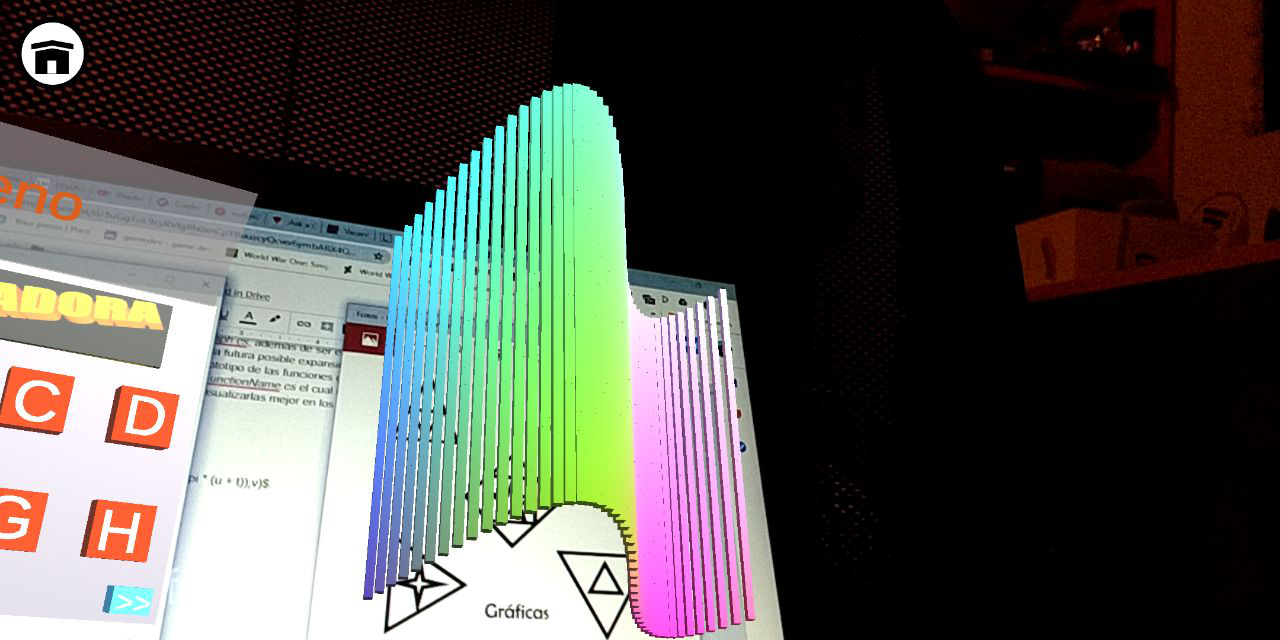
\includegraphics[width=0.5\textwidth]{figuras/graficas/seno.png}
\caption{\label{fig:graf_seno}Gráfica de la función Seno.}
\end{figure}
\FloatBarrier

\paragraph{Seno 2D}
Dado por la ecuación $f(u,v,t)=(u,Sen(\pi * (u + v+ t))*0.5,v)$. La Figura \ref{fig:graf_seno2d} es la gráfica de esta función, la cual es la opción B del menú.

\begin{figure}[hbt!]
\centering
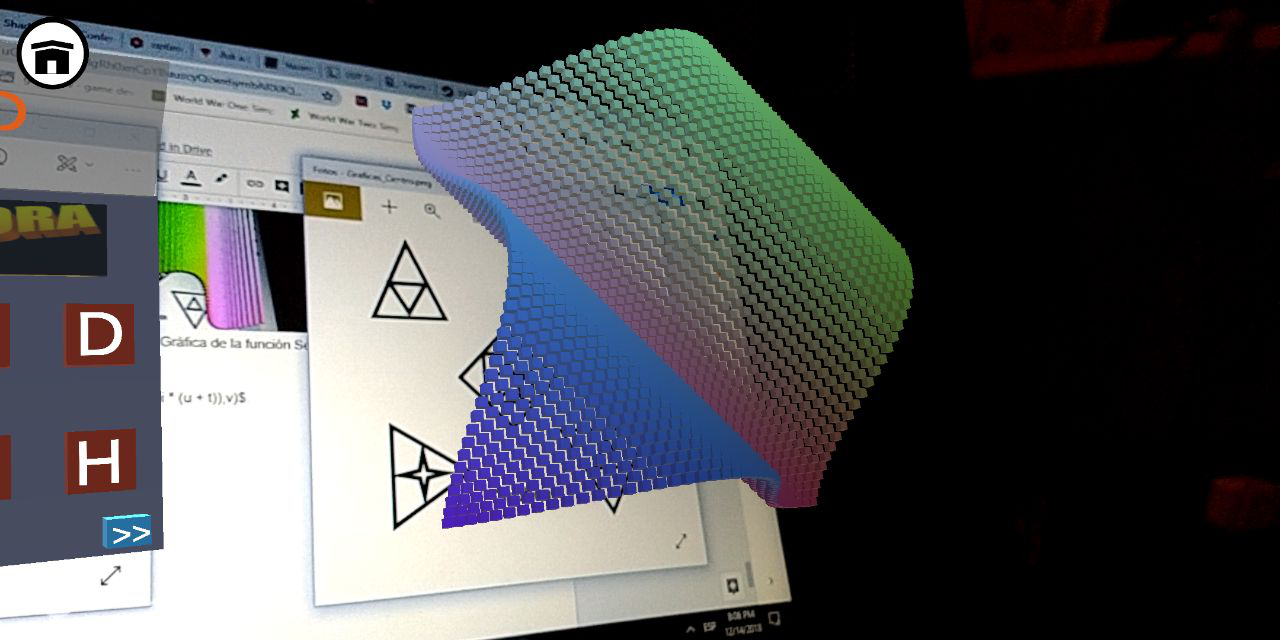
\includegraphics[width=0.5\textwidth]{figuras/graficas/seno2d.png}
\caption{\label{fig:graf_seno2d}Gráfica de la función Seno 2D.}
\end{figure}
\FloatBarrier

\paragraph{Media del Seno}
Dado por la ecuación $f(u,v,t)=(u,Sen(\pi * (u + t))/2+Sen(\pi * (v+ t))/2,v)$. La Figura \ref{fig:graf_media_seno} es la gráfica de esta función, la cual es la opción C del menú.

\begin{figure}[hbt!]
\centering
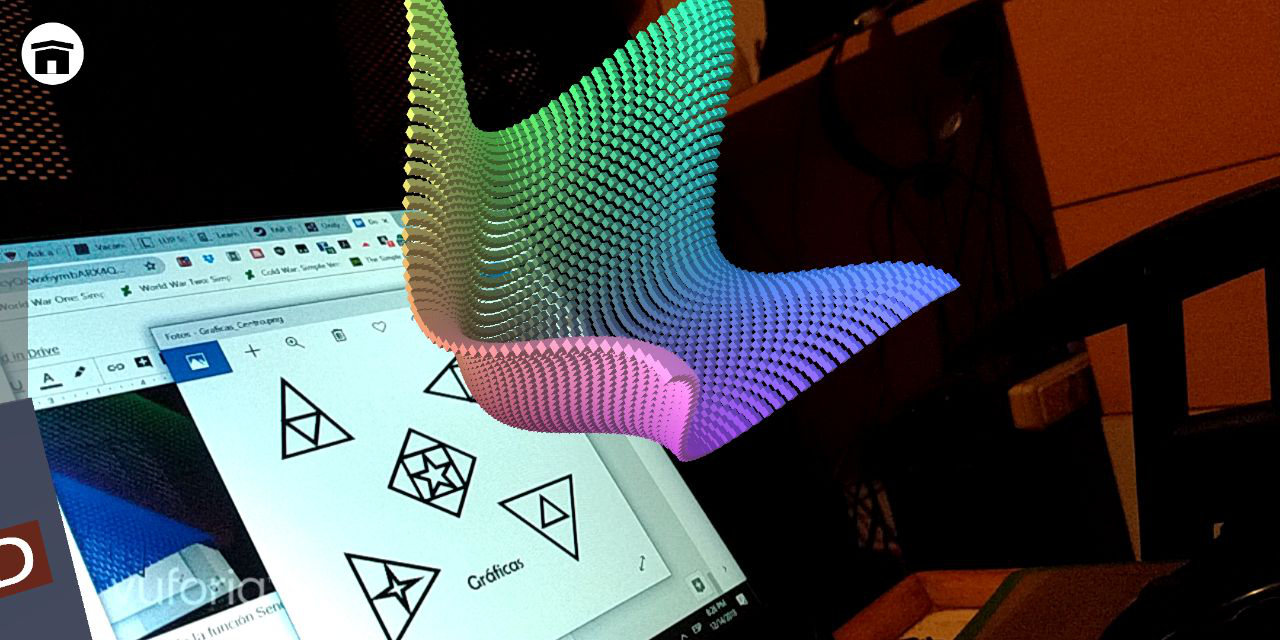
\includegraphics[width=0.5\textwidth]{figuras/graficas/media_seno.png}
\caption{\label{fig:graf_media_seno}Gráfica de la función Media del Seno.}
\end{figure}
\FloatBarrier

\paragraph{Multiseno}
Dado por la ecuación $f(u,v,t)=(u,Sen(\pi * (u + t))*2/3+Sen(2 * \pi * (v + 2 * t))/3,v)$. La Figura \ref{fig:graf_multiseno} es la gráfica de esta función, la cual es la opción D del menú.

\begin{figure}[hbt!]
\centering
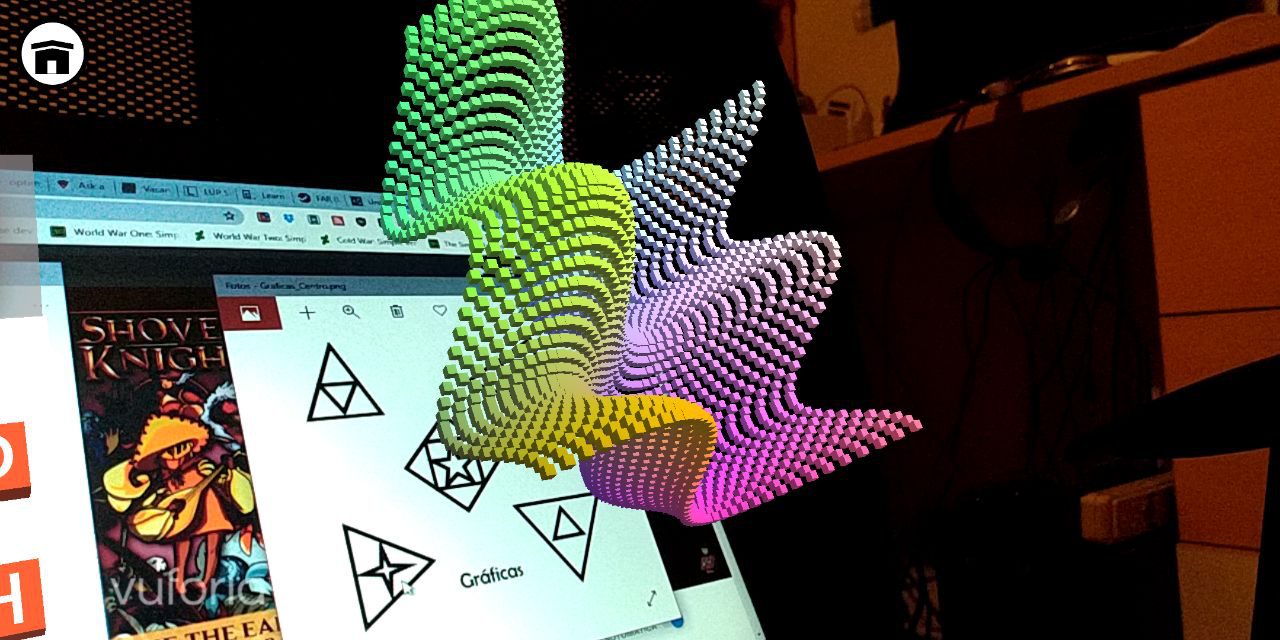
\includegraphics[width=0.5\textwidth]{figuras/graficas/multiseno.png}
\caption{\label{fig:graf_multiseno}Gráfica de la función Mutiseno.}
\end{figure}
\FloatBarrier

\paragraph{Multiseno 2D}
Dado por la ecuación $f(u,v,t)=(u, (4 * Sen(\pi * (u + v + t / 2)) + Sen(\pi * (u + t)) + Sen(2 * \pi * (v + 2 * t)) * 0.5) * 1 / 5.5,v)$. La Figura \ref{fig:graf_multiseno2d} es la gráfica de esta función, la cual es la opción E del menú.

\begin{figure}[hbt!]
\centering
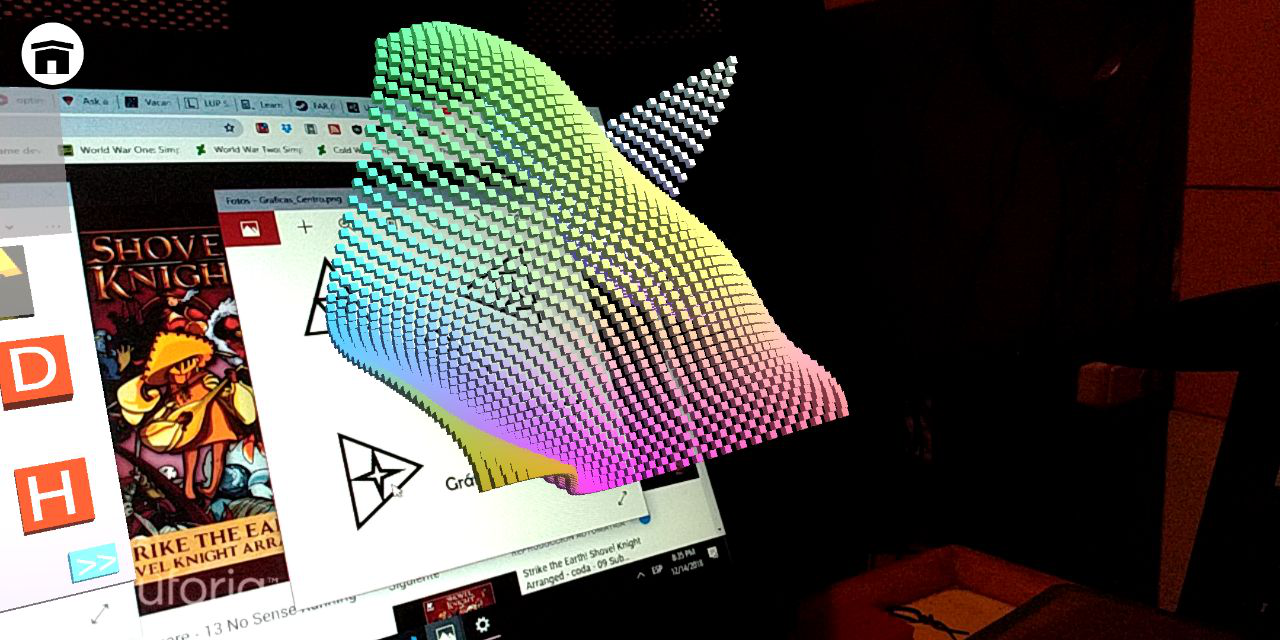
\includegraphics[width=0.5\textwidth]{figuras/graficas/multiseno2d.png}
\caption{\label{fig:graf_multiseno2d}Gráfica de la función Mutiseno 2D.}
\end{figure}
\FloatBarrier

\paragraph{Onda}
Dado por la ecuación $f(u,v,t)=(u, Sen(\pi * (4 * d - t))/(1 + 10 * d),v)$ donde $d=\sqrt{u * u + v * v}$. La Figura \ref{fig:graf_onda} es la gráfica de esta función, la cual es la opción F del menú.

\begin{figure}[hbt!]
\centering
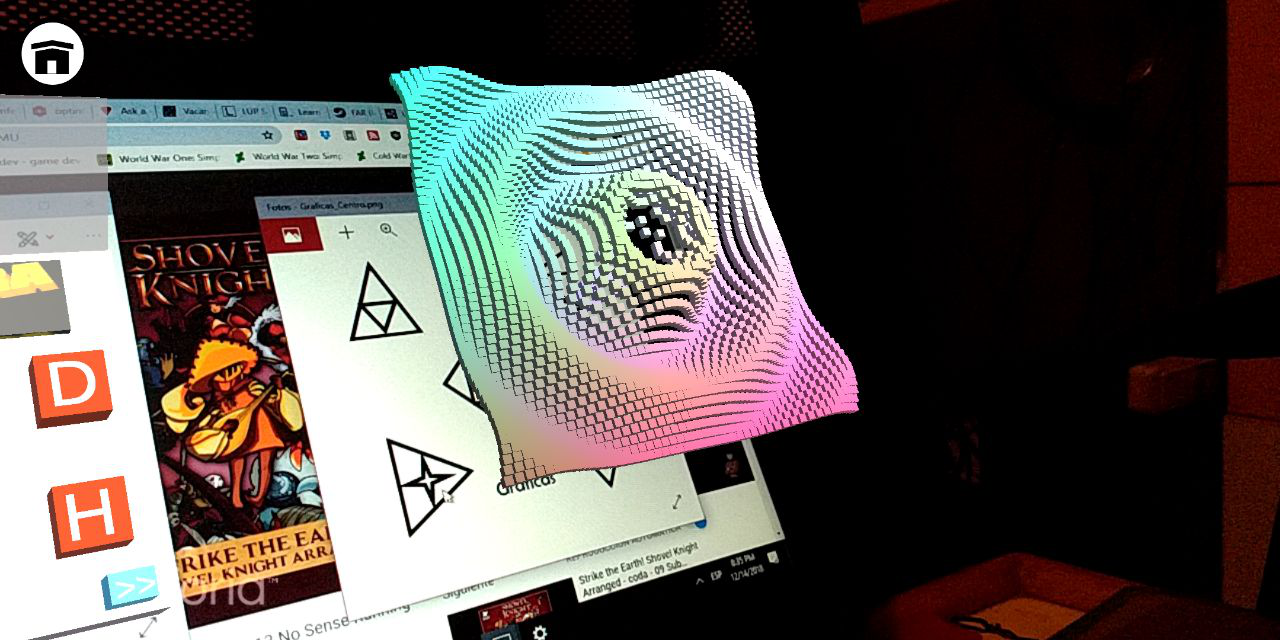
\includegraphics[width=0.5\textwidth]{figuras/graficas/onda.png}
\caption{\label{fig:graf_onda}Gráfica de la función Onda.}
\end{figure}
\FloatBarrier

\paragraph{Círculo}
Dado por la ecuación $f(u,v,t)=(Sen(\pi * u), 0,Cos(\pi * u))$. La Figura \ref{fig:graf_circulo} es la gráfica de esta función, la cual es la opción G del menú.

\begin{figure}[hbt!]
\centering
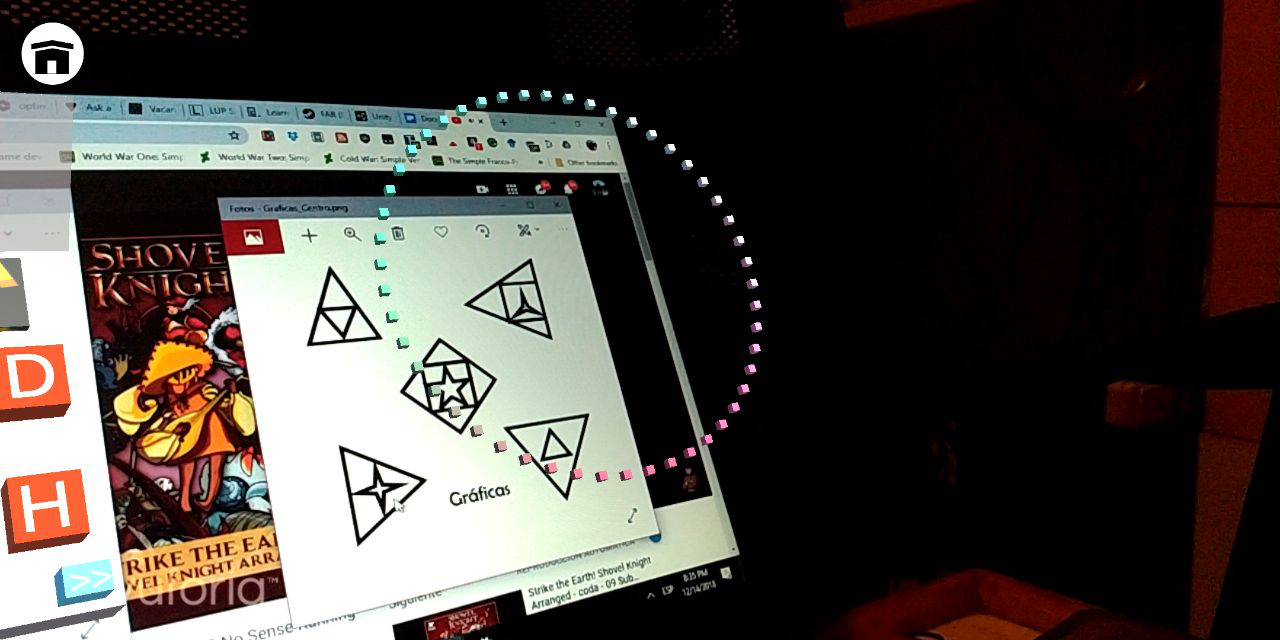
\includegraphics[width=0.5\textwidth]{figuras/graficas/circulo.png}
\caption{\label{fig:graf_circulo}Gráfica de la función Círculo.}
\end{figure}
\FloatBarrier

\paragraph{Remolino}
Dado por la ecuación $f(u,v,t)=(Sen(\pi * w), u, Cos(\pi * w))$ donde $w = u + t$. La Figura \ref{fig:graf_remolino} es la gráfica de esta función, la cual es la opción H del menú.

\begin{figure}[hbt!]
\centering
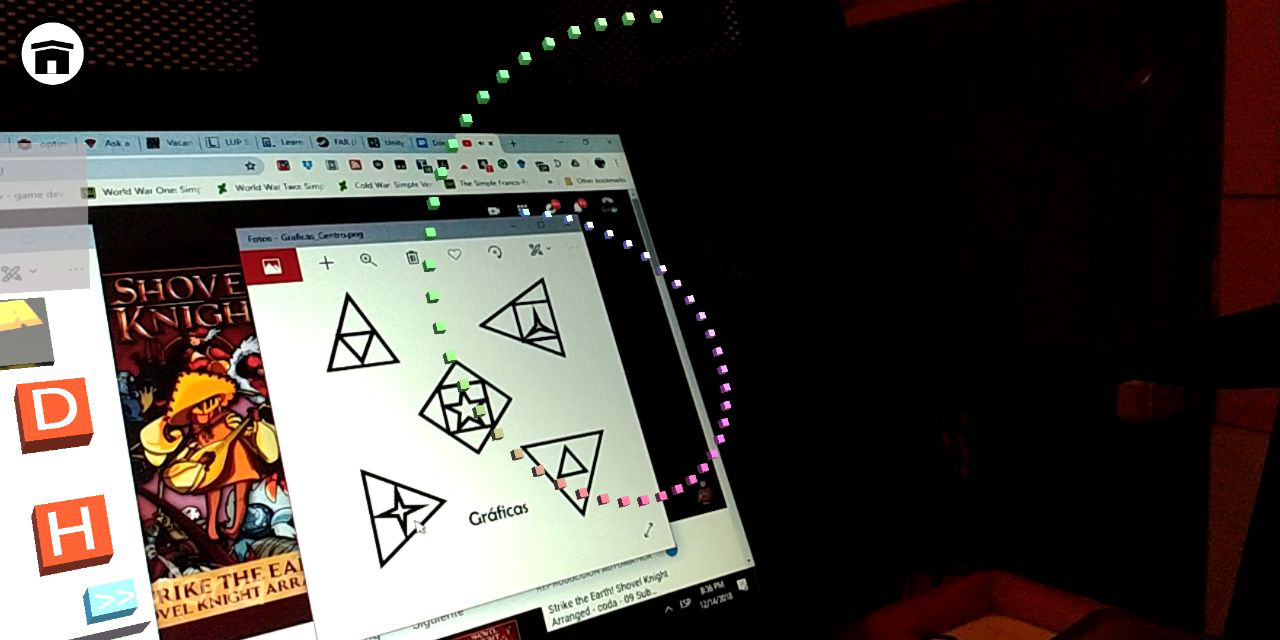
\includegraphics[width=0.5\textwidth]{figuras/graficas/remolino.png}
\caption{\label{fig:graf_remolino}Gráfica de la función Remolino.}
\end{figure}
\FloatBarrier

\paragraph{Cilindro}
Dado por la ecuación $f(u,v,t)=(r*Sen(\pi * u), v, r*Cos(\pi * u))$ donde $r = 1$. La Figura \ref{fig:graf_cilindro} es la gráfica de esta función, la cual es la opción I del menú.

\begin{figure}[hbt!]
\centering
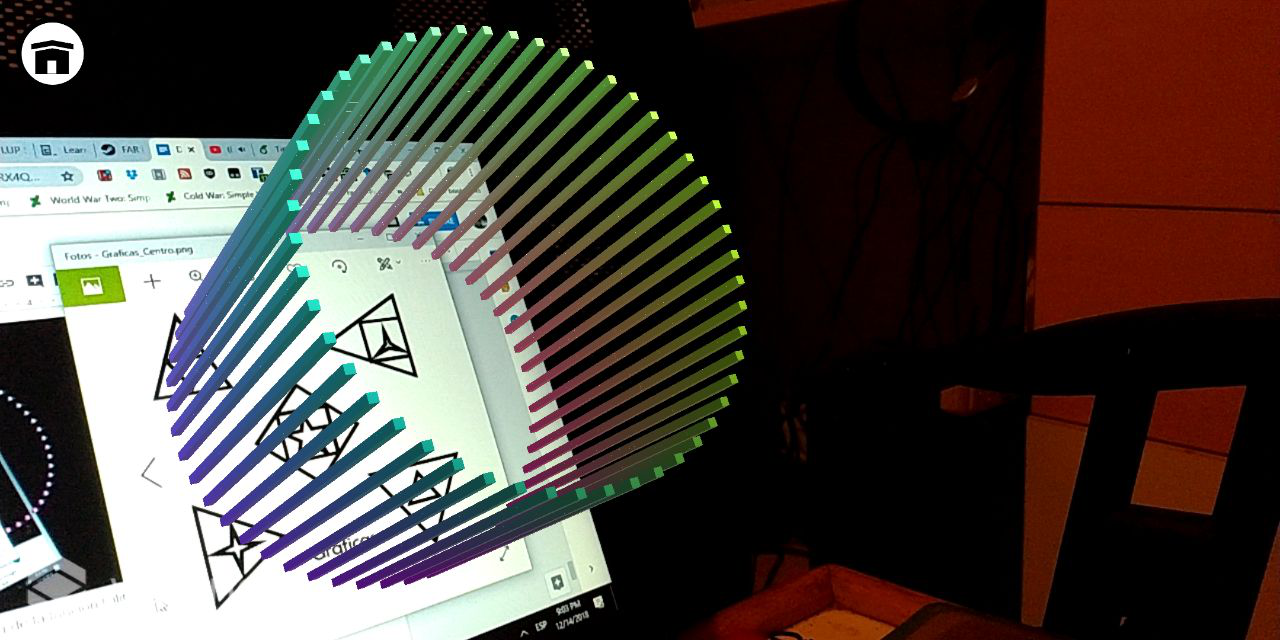
\includegraphics[width=0.5\textwidth]{figuras/graficas/cilindro.png}
\caption{\label{fig:graf_cilindro}Gráfica de la función Cilindro.}
\end{figure}
\FloatBarrier

\paragraph{Cilindro Tambaleante}
Dado por la ecuación $f(u,v,t)=(r*Sen(\pi * u), v, r*Cos(\pi * u))$ donde $r = 1 + Sen(6 * pi * u) * 0.2$. La Figura \ref{fig:graf_cilindro_tambaleante} es la gráfica de esta función, la cual es la opción J del menú.

\begin{figure}[hbt!]
\centering
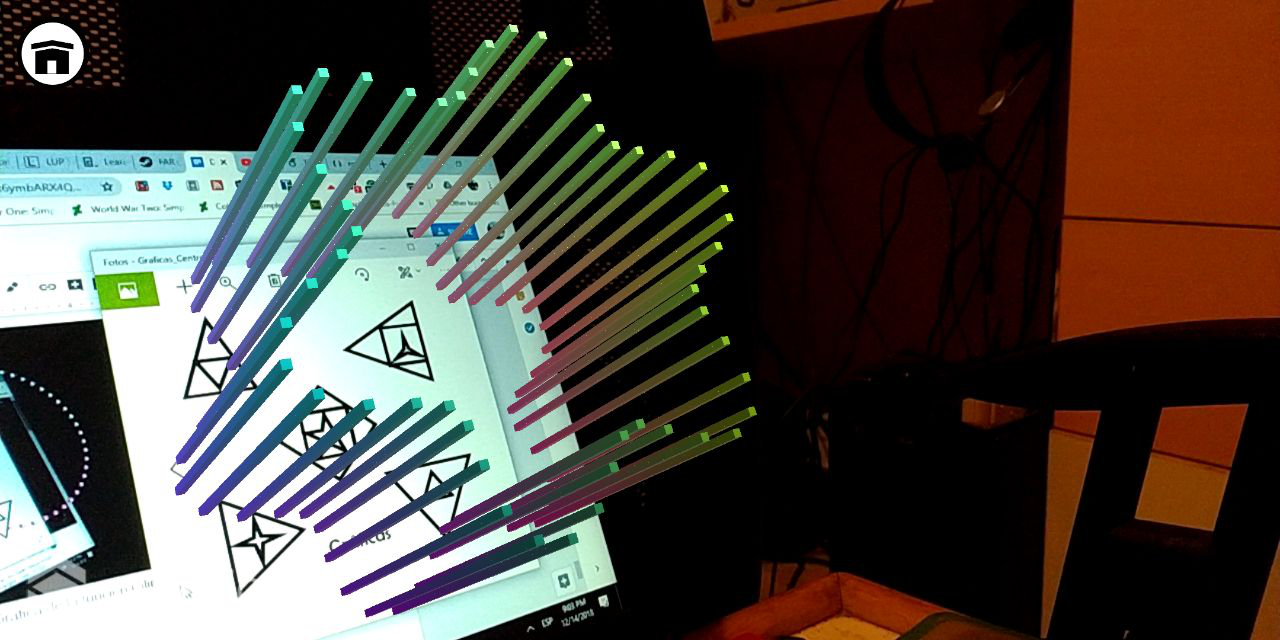
\includegraphics[width=0.5\textwidth]{figuras/graficas/cilindro_tambaleante.png}
\caption{\label{fig:graf_cilindro_tambaleante}Gráfica de la función Cilindro Tambaleante.}
\end{figure}
\FloatBarrier

\paragraph{Cilindro de Olla}
Dado por la ecuación $f(u,v,t)=(r*Sen(\pi * u), v, r*Cos(\pi * u))$ donde $r = 1 + Sen(2 * pi * v) * 0.2$. La Figura \ref{fig:graf_cilindro_olla} es la gráfica de esta función, la cual es la opción K del menú.

\begin{figure}[hbt!]
\centering
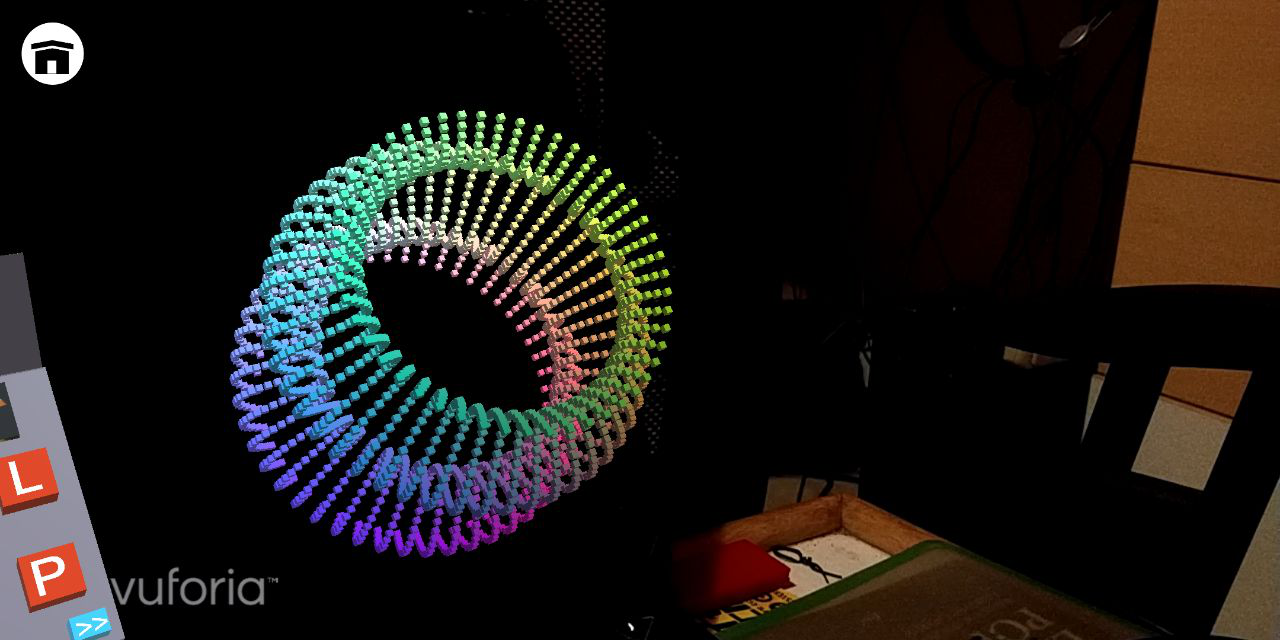
\includegraphics[width=0.5\textwidth]{figuras/graficas/cilindro_olla.png}
\caption{\label{fig:graf_cilindro_olla}Gráfica de la función Cilindro de Olla.}
\end{figure}
\FloatBarrier

\paragraph{Cilindro de Torsión}
Dado por la ecuación $f(u,v,t)=(r*Sen(\pi * u), v, r*Cos(\pi * u))$ donde $r = 0.8 + Sen(\pi * (6 * u + 2 * v + t)) * 0.2$. La Figura \ref{fig:graf_cilindro_torsion} es la gráfica de esta función, la cual es la opción L del menú.

\begin{figure}[hbt!]
\centering
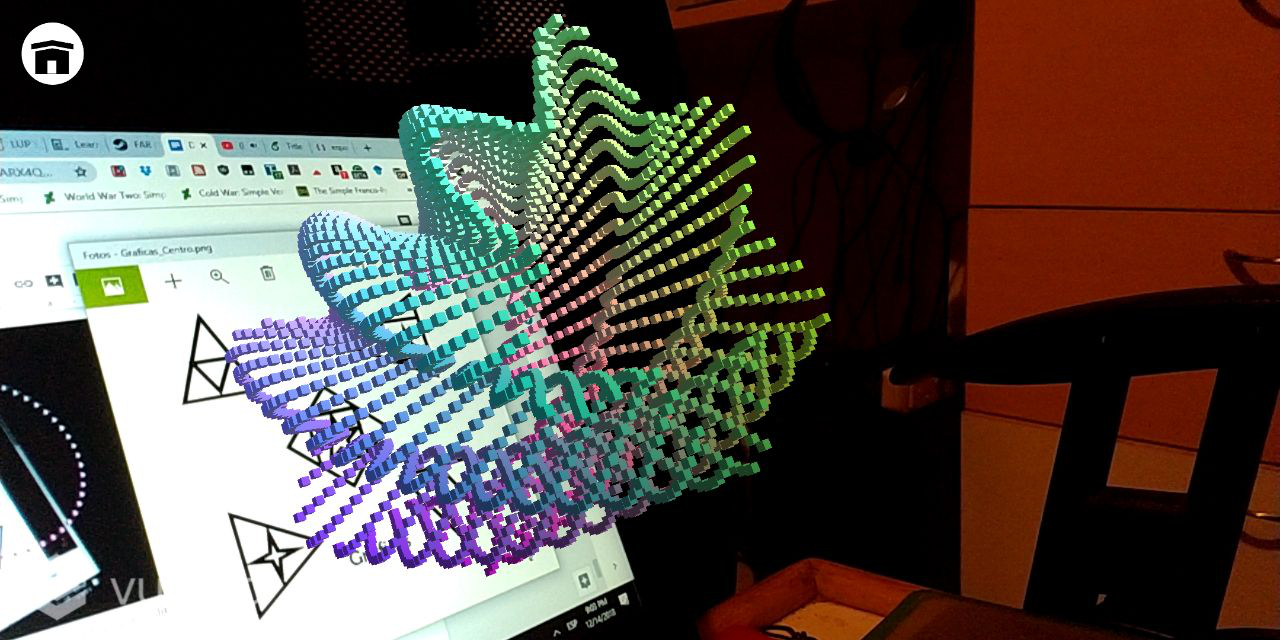
\includegraphics[width=0.5\textwidth]{figuras/graficas/cilindro_torsion.png}
\caption{\label{fig:graf_cilindro_torsion}Gráfica de la función Cilindro de Torsión.}
\end{figure}
\FloatBarrier

\paragraph{Esfera}
Dado por la ecuación $f(u,v,t)=(r*Sen(\pi * u), Sen(\pi * 0.5 * v), r*Cos(\pi * u))$ donde $r = Cos(\pi * 0.5 * v)$. La Figura \ref{fig:graf_esfera} es la gráfica de esta función, la cual es la opción M del menú.

\begin{figure}[hbt!]
\centering
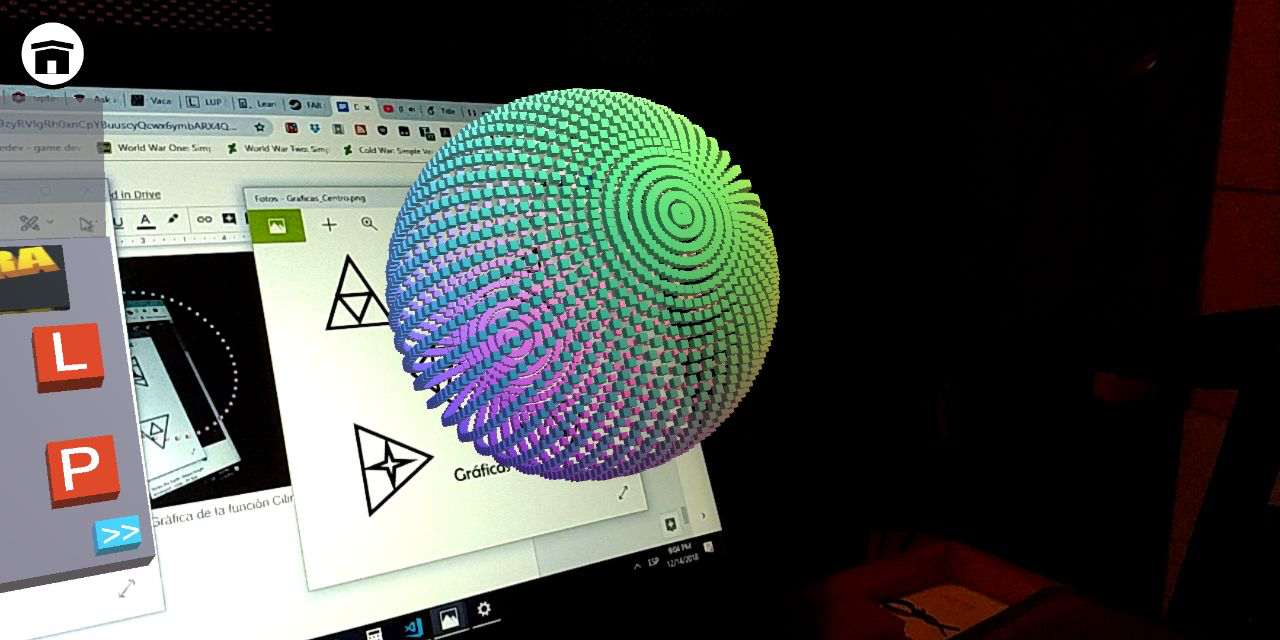
\includegraphics[width=0.5\textwidth]{figuras/graficas/esfera.png}
\caption{\label{fig:graf_esfera}Gráfica de la función Esfera.}
\end{figure}
\FloatBarrier

\paragraph{Esfera Cardioide}
Dado por la ecuación $f(u,v,t)=(r*Sen(\pi * u), v, r*Cos(\pi * u))$ donde $r = Cos(\pi * 0.5 * v)$. La Figura \ref{fig:graf_esfera_cardioide} es la gráfica de esta función, la cual es la opción N del menú.

\begin{figure}[hbt!]
\centering
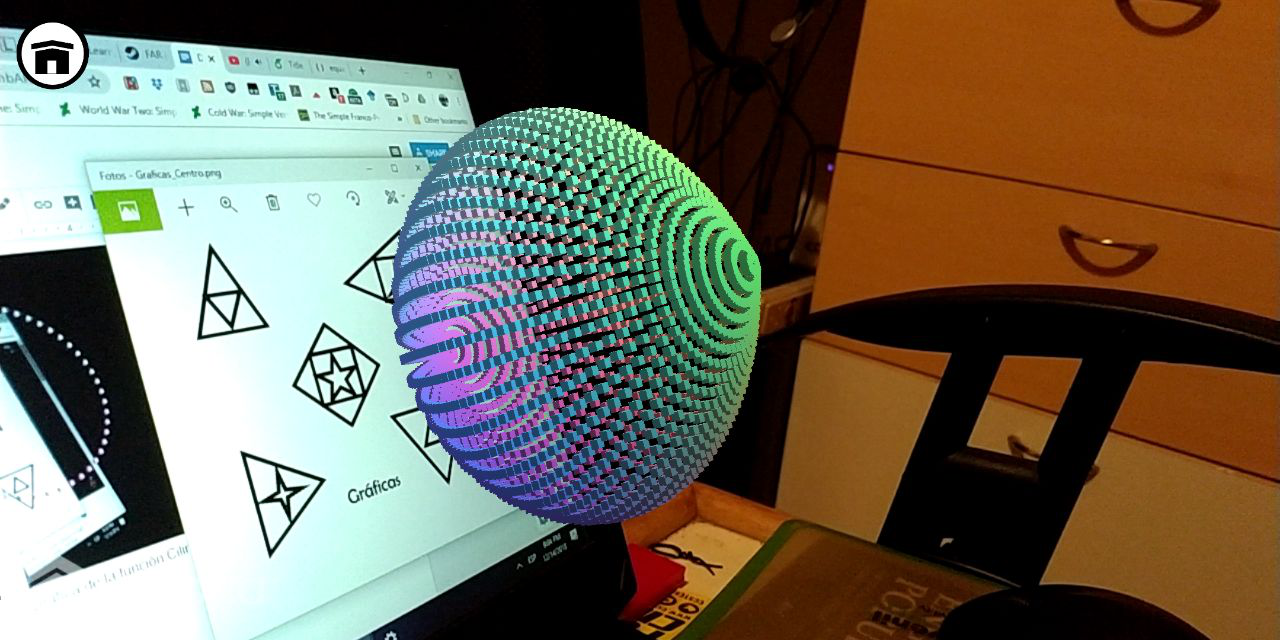
\includegraphics[width=0.5\textwidth]{figuras/graficas/esfera_cardioide.png}
\caption{\label{fig:graf_esfera_cardioide}Gráfica de la función Esfera Cardioide.}
\end{figure}
\FloatBarrier

\paragraph{Esfera Pulsante}
Dado por la ecuación $f(u,v,t)=(s*Sen(\pi * u), r * Sen(\pi * 0.5 * v), s*Cos(\pi * u))$ donde $s = r*Cos(\pi * 0.5 * v)$ y $r=0.8 + Sen(\pi * (6 * u + t)) * 0.1 + Sen(\pi * (4 * v + t)) * 0.1$. La Figura \ref{fig:graf_esfera_pulsante} es la gráfica de esta función, la cual es la opción O del menú.

\begin{figure}[hbt!]
\centering
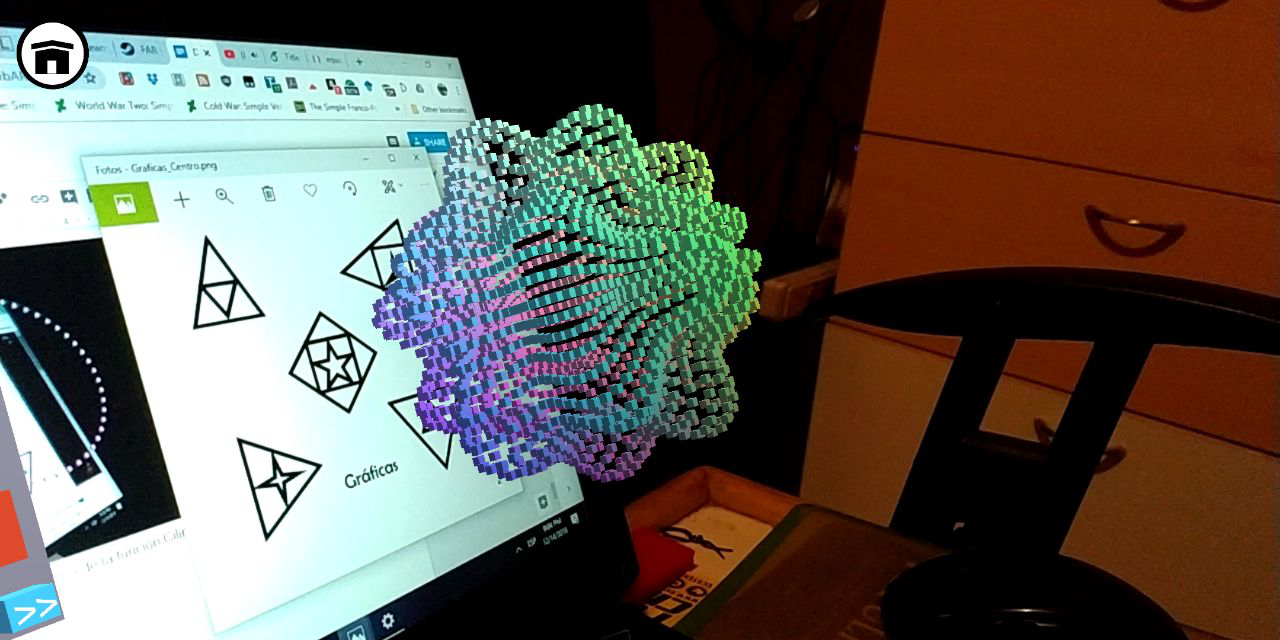
\includegraphics[width=0.5\textwidth]{figuras/graficas/esfera_pulsante.png}
\caption{\label{fig:graf_esfera_pulsante}Gráfica de la función Esfera Pulsante.}
\end{figure}
\FloatBarrier

\paragraph{Toroide Exterior}
Dado por la ecuación $f(u,v,t)=(s*Sen(\pi * u), Sen(\pi * 0.5 * v), s*Cos(\pi * u))$ donde $s = Cos(\pi * 0.5 * v) + 0.5$. La Figura \ref{fig:graf_toroide_exterior} es la gráfica de esta función, la cual es la opción P del menú.

\begin{figure}[hbt!]
\centering
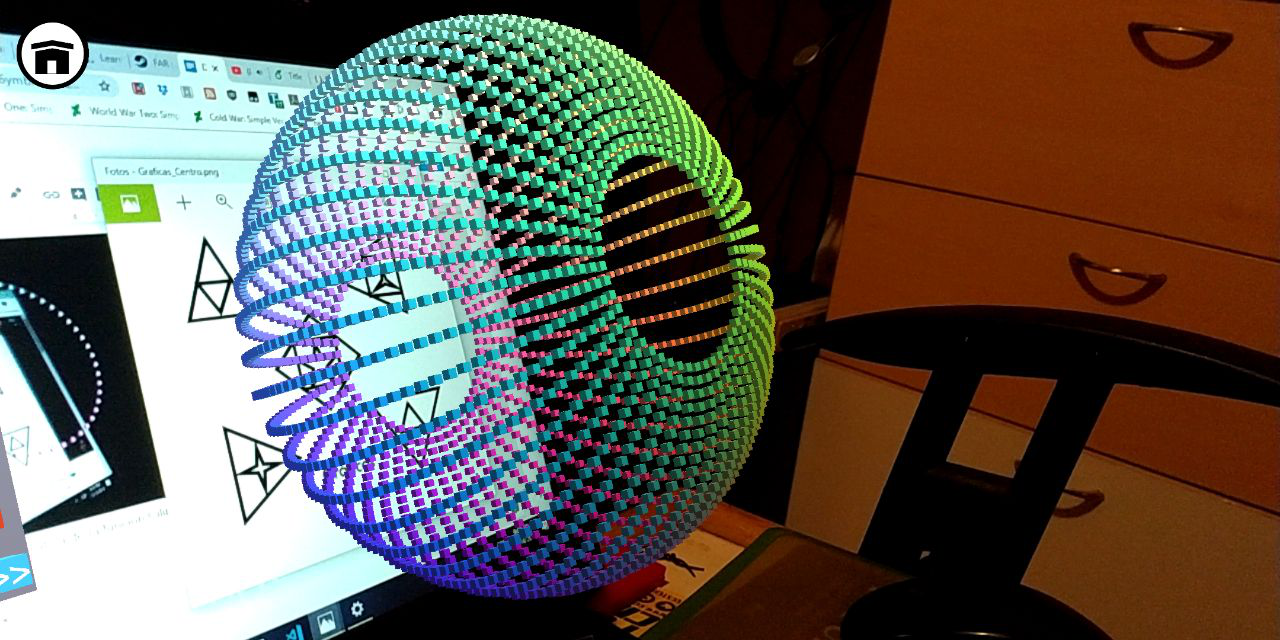
\includegraphics[width=0.5\textwidth]{figuras/graficas/toroide_exterior.png}
\caption{\label{fig:graf_toroide_exterior}Gráfica de la función Toroide Exterior.}
\end{figure}
\FloatBarrier

\paragraph{Toroide de Intersección}
Dado por la ecuación $f(u,v,t)=(s*Sen(\pi * u), Sen(\pi *  v), s*Cos(\pi * u))$ donde $s = Cos(\pi * 0.5 * v) + 0.5$. La Figura \ref{fig:graf_toroide_interseccion} es la gráfica de esta función, la cual es la opción Q del menú.

\begin{figure}[hbt!]
\centering
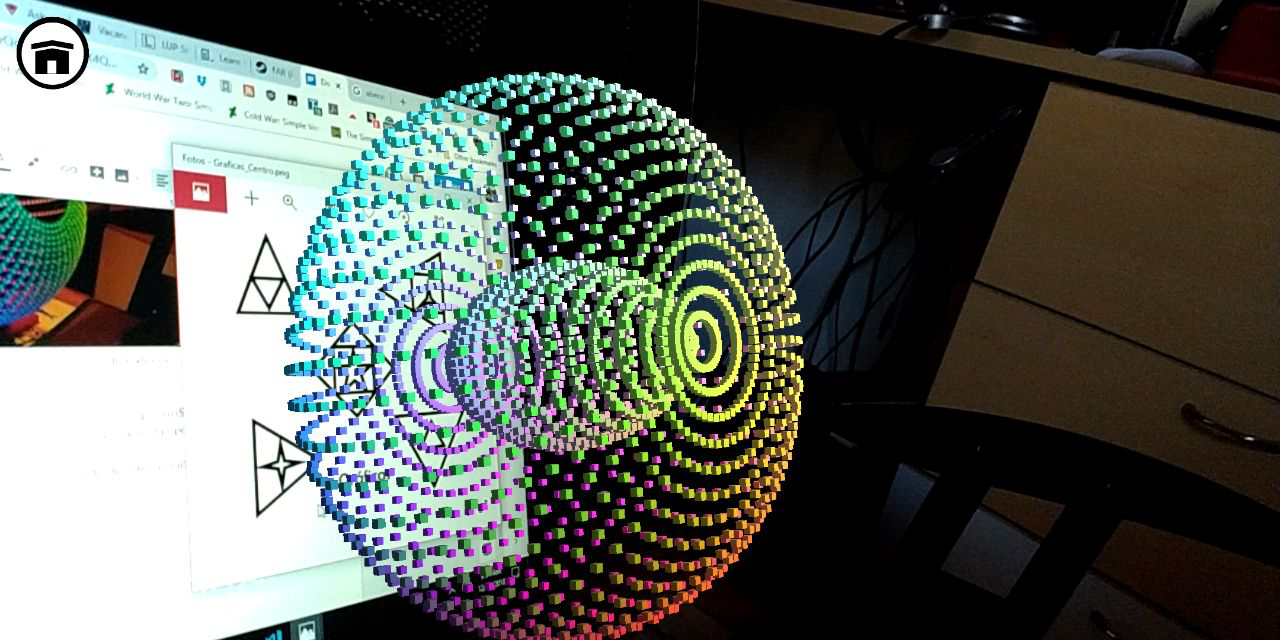
\includegraphics[width=0.5\textwidth]{figuras/graficas/toroide_interseccion.png}
\caption{\label{fig:graf_toroide_interseccion}Gráfica de la función Toroide de Intersección.}
\end{figure}
\FloatBarrier

\paragraph{Toroide de Cuerno}
Dado por la ecuación $f(u,v,t)=(s*Sen(\pi * u), Sen(\pi *  v), s*Cos(\pi * u))$ donde $s = Cos(\pi * v)+r_1$ y $r_1 = 1$. La Figura \ref{fig:graf_toroide_cuerno} es la gráfica de esta función, la cual es la opción R del menú.

\begin{figure}[hbt!]
\centering
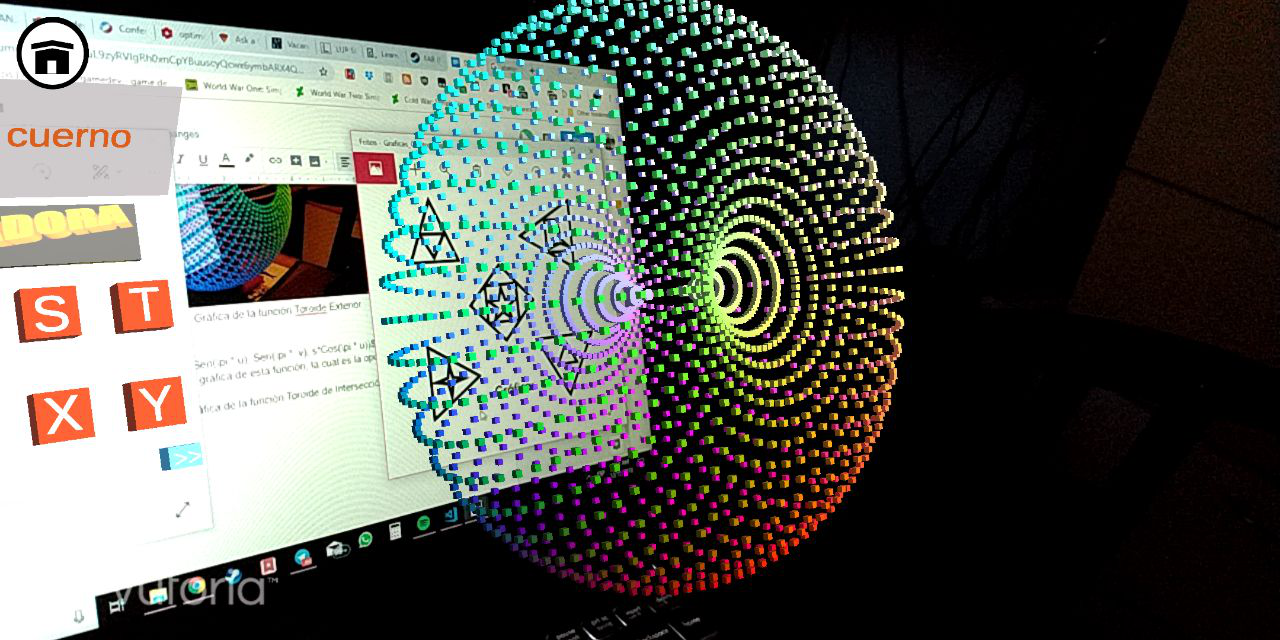
\includegraphics[width=0.5\textwidth]{figuras/graficas/toroide_cuerno.png}
\caption{\label{fig:graf_toroide_cuerno}Gráfica de la función Toroide de Cuerno.}
\end{figure}
\FloatBarrier

\paragraph{Toroide Anidado}
Dado por la ecuación $f(u,v,t)=(s*Sen(\pi * u), r_2 * Sen(\pi *  v), s*Cos(\pi * u))$ donde $s = Cos(\pi * v)$, $r_1 = 1$ y $r_2 = 0.5$. La Figura \ref{fig:graf_toroide_anidado} es la gráfica de esta función, la cual es la opción S del menú.

\begin{figure}[hbt!]
\centering
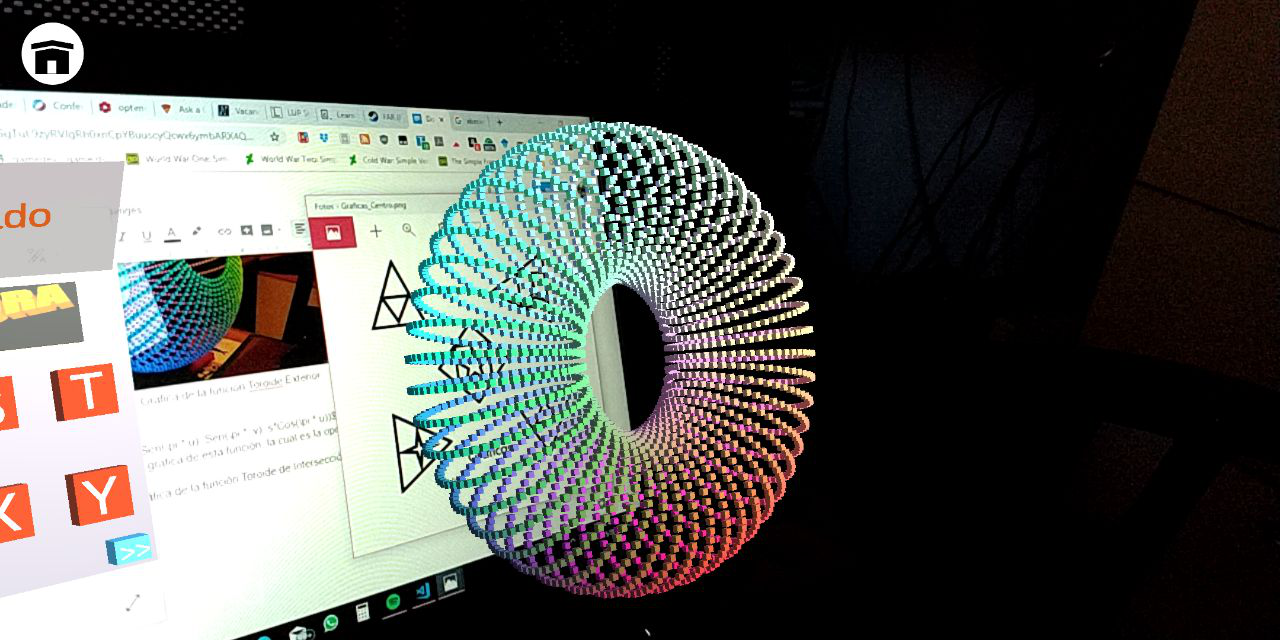
\includegraphics[width=0.5\textwidth]{figuras/graficas/toroide_anidado.png}
\caption{\label{fig:graf_toroide_anidado}Gráfica de la función Toroide Anidado.}
\end{figure}
\FloatBarrier

\paragraph{Toroide Estrella}
Dado por la ecuación $f(u,v,t)=(s*Sen(\pi * u), r_2 * Sen(\pi *  v), s*Cos(\pi * u))$ donde $s = Cos(\pi * v)$, $r_1 = 10.65 + Sen(\pi * (6 * u + t)) * 0.1$ y $r_2 = 0.2 + Sen(\pi * (4 * v + t)) * 0.05$. La Figura \ref{fig:graf_toroide_estrella} es la gráfica de esta función, la cual es la opción T del menú.

\begin{figure}[hbt!]
\centering
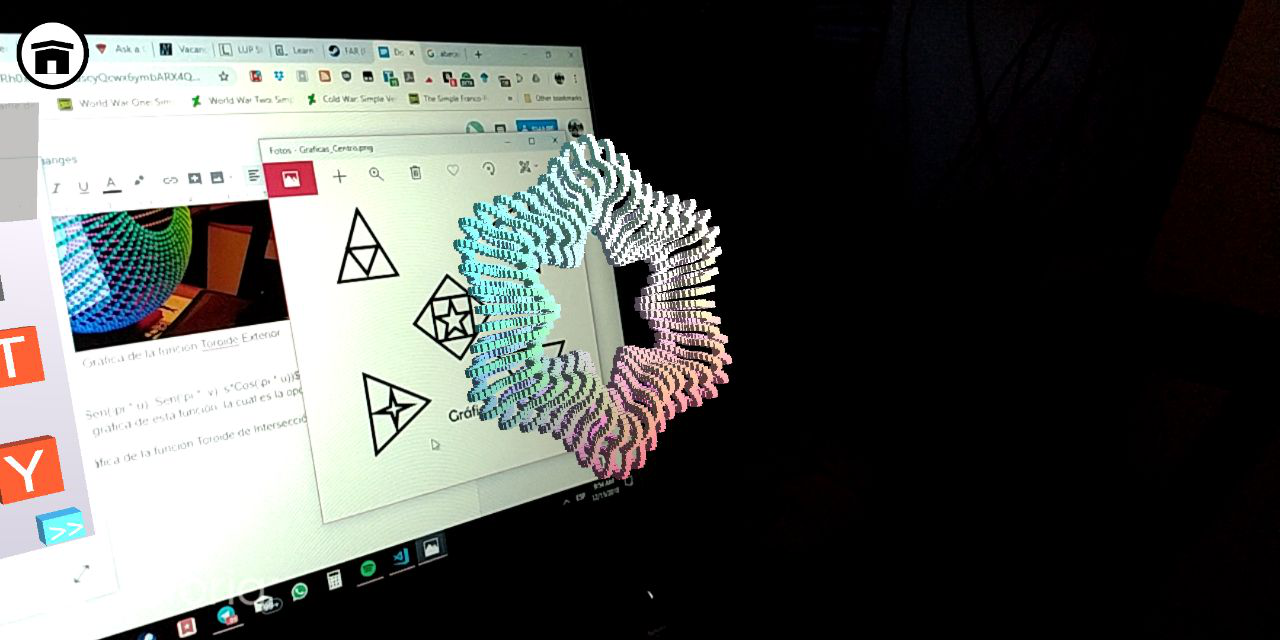
\includegraphics[width=0.5\textwidth]{figuras/graficas/toroide_estrella.png}
\caption{\label{fig:graf_toroide_estrella}Gráfica de la función Toroide Estrella.}
\end{figure}
\FloatBarrier

\paragraph{Banda de Mobius}
Dado por la ecuación $f(u,v,t)=(te*Cos(nu),te*Sen(nu),halfnv*Sen(halfnu))$ donde $te = 1 + halfnv * Cos(halfnu)$, $nu = 2 * halfnu$, $halfnv = v - 0.5$ y $halfnu = (u + t * 0.05) * \pi$ . La Figura \ref{fig:graf_mobius} es la gráfica de esta función, la cual es la opción U del menú.

\begin{figure}[hbt!]
\centering
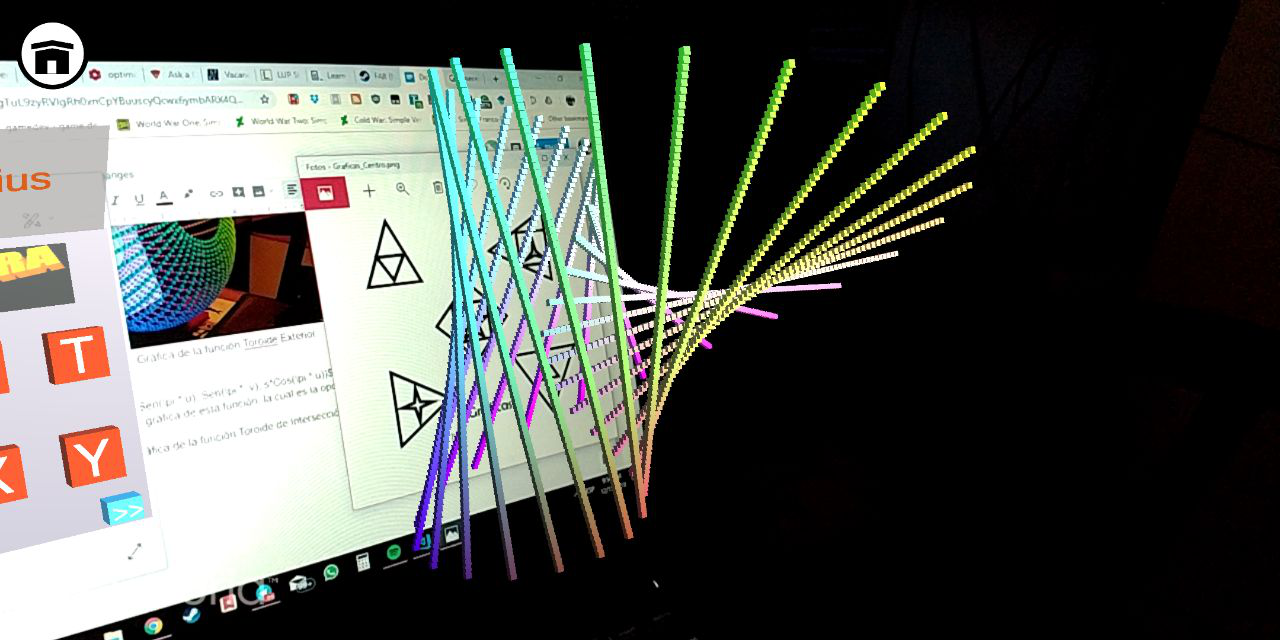
\includegraphics[width=0.5\textwidth]{figuras/graficas/mobius.png}
\caption{\label{fig:graf_mobius}Gráfica de la función Banda de Mobius.}
\end{figure}
\FloatBarrier

\paragraph{Banda Especial de Mobius}
Dado por la ecuación $f(u,v,t)=(te*Cos(nu),te*Sen(nu),halfnv*Sen(halfnu))$ donde $te = 1 + halfnv * Cos(halfnu)$, $nu = 2 * halfnu$, $halfnv = (v - 0.5) * Cos(\pi * (t * 0.05 + v)) * Cos(\pi * (t * 0.1f + u)) * Cos(\pi * (t * 0.2 + u + v))$ y $halfnu = (u + t * 0.05) * \pi$ . La Figura \ref{fig:graf_mobius_especial} es la gráfica de esta función, la cual es la opción V del menú.

\begin{figure}[hbt!]
\centering
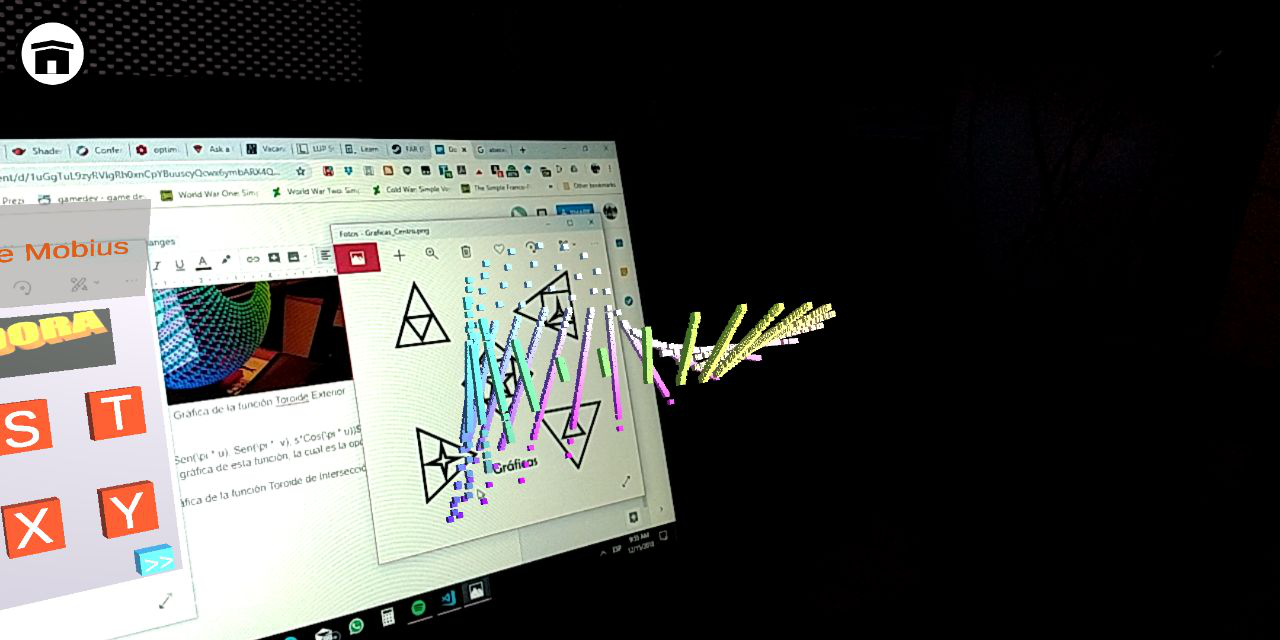
\includegraphics[width=0.5\textwidth]{figuras/graficas/mobius_especial.png}
\caption{\label{fig:graf_mobius_especial}Gráfica de la función Banda Especial de Mobius.}
\end{figure}
\FloatBarrier

\paragraph{Botella de Klein Estática}
Dado por la ecuación $f(u,v,t)=(-2/15 * cu * (3 * cv - 30 * su + 90 * cu^4 * su - 60 * cu^6 * su + 5 * cu * cv * su), -1/15 * su * (3 * cv - 3 * cu^2 * cv - 48 * cu^4 * cv + 48 * cu^6 * cv - 60 * su + 5 * cu * cv * su - 5 * cu^3 * cv * su - 80 * cu^5 * cv * sv + 80 * cu^7 * cv * su) -2, 2/15 * (3 + 5 * cu * su) * sv)$ donde $sv = Sen(nv)$, $cv = Cos(nv)$, $su = Sen(nu)$, $cu = Cos(nu)$, $nv = v * \pi * 2$ y $nu = u * \pi$. La Figura \ref{fig:graf_klein_estatico} es la gráfica de esta función, la cual es la opción W del menú.

\begin{figure}[hbt!]
\centering
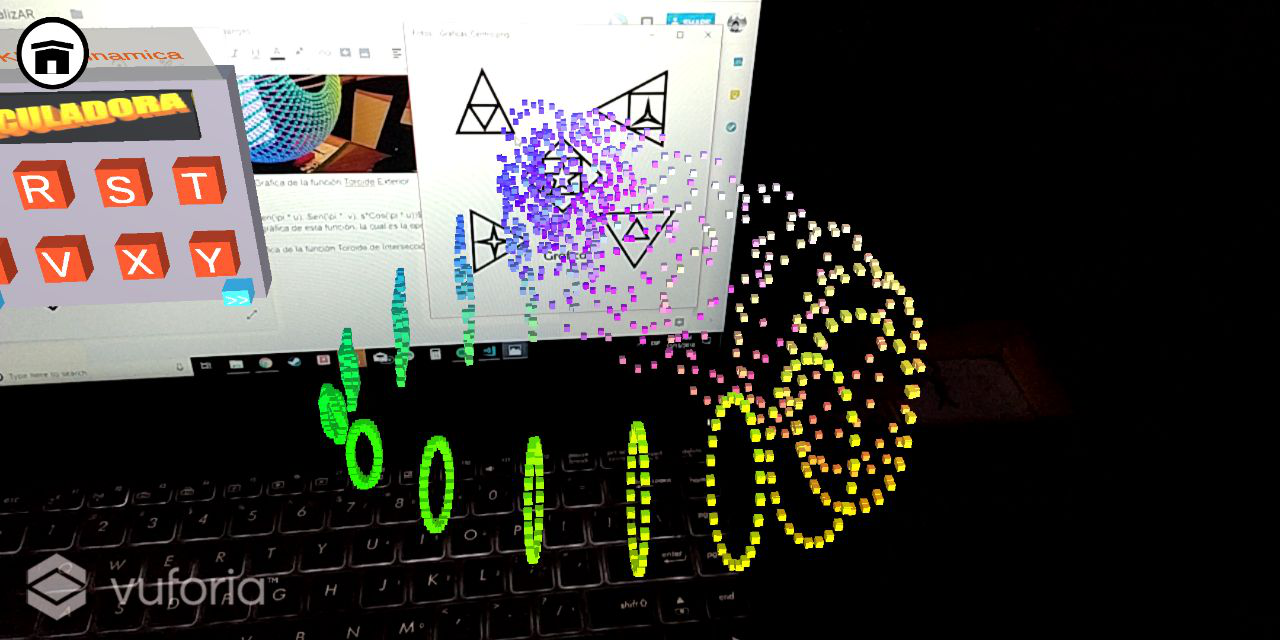
\includegraphics[width=0.5\textwidth]{figuras/graficas/klein_estatico.png}
\caption{\label{fig:graf_klein_estatico}Gráfica de la función Botella de Klein Estática.}
\end{figure}
\FloatBarrier

\paragraph{Botella de Klein Dinámica}
Dado por la ecuación $f(u,v,t)=(-2/15 * cu * (3 * cv - 30 * su + 90 * cu^4 * su - 60 * cu^6 * su + 5 * cu * cv * su), -1/15 * su * (3 * cv - 3 * cu^2 * cv - 48 * cu^4 * cv + 48 * cu^6 * cv - 60 * su + 5 * cu * cv * su - 5 * cu^3 * cv * su - 80 * cu^5 * cv * sv + 80 * cu^7 * cv * su) -2, 2/15 * (3 + 5 * cu * su) * sv)$ donde $sv = Sen(nv)$, $cv = Cos(nv)$, $su = Sen(nu)$, $cu = Cos(nu)$, $nv = (v+ t * 0.2) * \pi * 2$ y $nu = (u+ t * 0.05) * \pi$. La Figura \ref{fig:graf_klein_dinamico} es la gráfica de esta función, la cual es la opción X del menú.

\begin{figure}[hbt!]
\centering
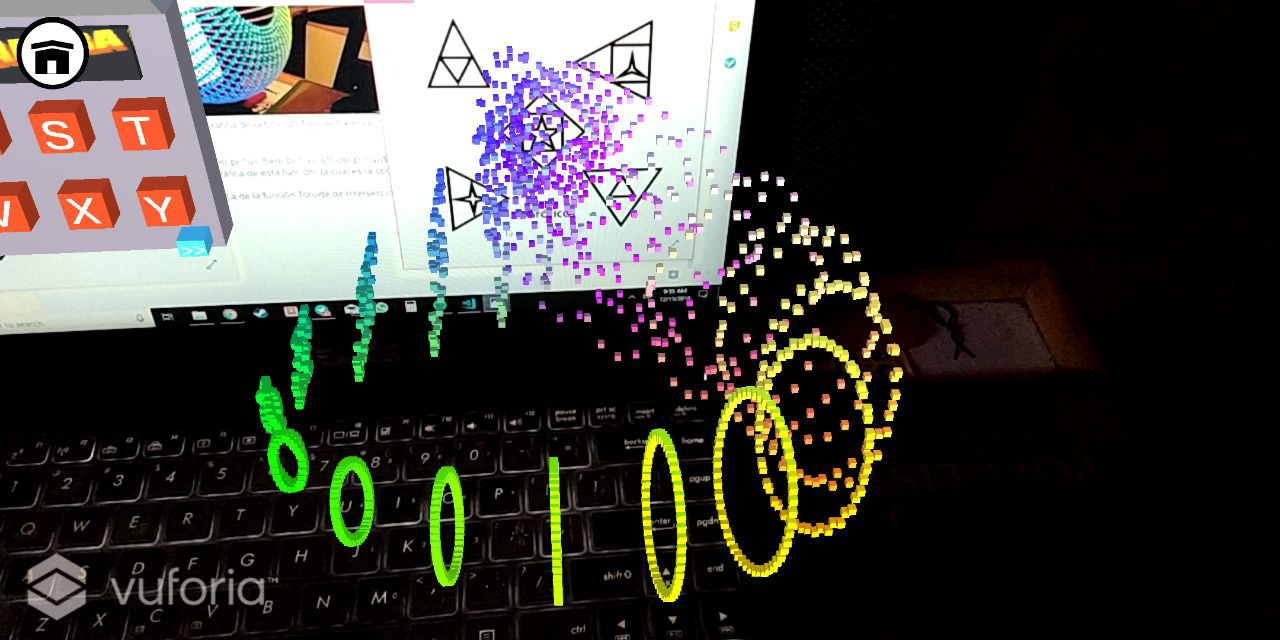
\includegraphics[width=0.5\textwidth]{figuras/graficas/klein_dinamico.png}
\caption{\label{fig:graf_klein_dinamico}Gráfica de la función Botella de Klein Dinámica.}
\end{figure}
\FloatBarrier

\bibliographystyle{plain}
\bibliography{references}
\end{document} to your LaTeX file where you want your
% title page.
%
%%%%%%%%%%%%%%%%%%%%%%%%%%%%%%%%%%%%%%%%%
%\title{Title page with logo}
%----------------------------------------------------------------------------------------
%	PACKAGES AND OTHER DOCUMENT CONFIGURATIONS
%----------------------------------------------------------------------------------------

\documentclass[12pt]{report}
\setcounter{tocdepth}{4}
\setcounter{secnumdepth}{4}
\usepackage[spanish]{babel}
\usepackage[utf8]{inputenc}
\usepackage{amsmath}
\usepackage{graphicx}
\usepackage[colorinlistoftodos]{todonotes}
\usepackage{hyperref}
\usepackage{acronym}
\usepackage{fancyhdr}
\usepackage{placeins}
\usepackage{amssymb}
\usepackage{etoolbox}
\usepackage{subfig}

\addto\captionsspanish{% Replace "english" with the language you use
  \renewcommand{\contentsname}%
    {Índice General}%
  \renewcommand{\listfigurename}%
    {Índice de Figuras}%
  \renewcommand{\listtablename}%
    {Índice de Tablas}%
  \renewcommand{\bibname}%
    {Referencias}%
  \renewcommand{\thechapter}{\Roman{chapter}}
  \renewcommand{\thesection}{\arabic{chapter}.\arabic{section}}
  \renewcommand{\thefigure}{\arabic{chapter}.\arabic{figure}}
  \renewcommand{\theequation}{\arabic{chapter}.\arabic{equation}}
}

\makeatletter
\def\@makechapterhead#1{%
  %%%%\vspace*{50\p@}% %%% removed!
  {\parindent \z@ \centering \normalfont
    \ifnum \c@secnumdepth >\m@ne
        \LARGE\bfseries \MakeUppercase{\@chapapp}\space \thechapter % <--- uppercase
        \par\nobreak
        \vskip 0\p@
    \fi
    \interlinepenalty\@M
    \Large \bfseries \MakeUppercase{#1}\par\nobreak
    \vskip 30\p@
  }}
\def\@makeschapterhead#1{%
  %%%%%\vspace*{50\p@}% %%% removed!
  {\parindent \z@ \centering
    \normalfont
    \interlinepenalty\@M
    \Large \bfseries  \MakeUppercase{#1}\par\nobreak
    \vskip 30\p@
  }}
\makeatother

\pagestyle{fancy}
\fancyhf{}
\fancyheadoffset{0cm}
\renewcommand{\headrulewidth}{0pt} 
\renewcommand{\footrulewidth}{0pt}
\fancyhead[R]{\thepage}
\fancypagestyle{plain}{%
   \fancyhf{}%
   \fancyhead[R]{\thepage}%
}

\fancypagestyle{chapterstart}{%
  \renewcommand{\headrulewidth}{0pt}%
  \fancyhf{}%
}

% \patchcmd{\chapter}{plain}{chapterstart}{}{}


\begin{document}

\begin{titlepage}

\newcommand{\HRule}{\rule{\linewidth}{0.5mm}} % Defines a new command for the horizontal lines, change thickness here



\center % Center everything on the page
 
%----------------------------------------------------------------------------------------
%	HEADING SECTIONS
%----------------------------------------------------------------------------------------

\includegraphics[width=0.15\textwidth]{figuras/logo_usb.png}\\[0.3cm]
\textsc{\bfseries UNIVERSIDAD SIMÓN BOLÍVAR}\\
\textsc{\bfseries DECANATO DE ESTUDIOS PROFESIONALES}\\
\textsc{\bfseries COORDINACIÓN DE INGENIERÍA DE COMPUTACIÓN}\\[4cm] % Name of your university/college

%----------------------------------------------------------------------------------------
%	TITLE SECTION
%----------------------------------------------------------------------------------------


{ \LARGE \bfseries VisualizAR}\\[3cm] % Title of your document
 
%----------------------------------------------------------------------------------------
%	AUTHOR SECTION
%----------------------------------------------------------------------------------------

% If you don't want a supervisor, uncomment the two lines below and remove the section above
\normalfont Por\\[0.3cm]
Christian Oliveros 13-11000\\% Your name
Alexander Romero 13-11274\\[2cm] % Your name

Realizado con la asesoria de:\\
Angela Di Serio\\[1cm]

EP-4793 Mini Proyecto de Desarrollo de Software\\[1cm]

%----------------------------------------------------------------------------------------
%	DATE SECTION
%----------------------------------------------------------------------------------------

{\bfseries Sartenejas, \today}\\[2cm] % Date, change the \today to a set date if you want to be precise

%----------------------------------------------------------------------------------------
%	LOGO SECTION
%----------------------------------------------------------------------------------------

 % Include a department/university logo - this will require the graphicx package
 
%----------------------------------------------------------------------------------------

\vfill % Fill the rest of the page with whitespace

\end{titlepage}

\pagenumbering{roman}
%\begin{abstract}
%Your abstract. \ac{API}
%
%\ac{API}
%\end{abstract}

\tableofcontents
\listoffigures
%\listoftables

\chapter*{Lista de Acrónimos}
\begin{acronym}
	\acro{USB}[USB]{Universidad Sim\'on Bol\'ivar}
	\acro{DEP}[DEP]{Decanato de Estudios Profesionales}
	\acro{PDF}[PDF]{\textit{Portable Document Format}, Documento en Formato Portable\copyright}
	\acro{3D}[3D]{\textit{Three Dimensions}, Tres Dimensiones}
	\acro{API}[API]{\textit{Application Programming Interface}, Interfaz de Programación de Aplicaciones}
	\acro{RGB}[RGB]{\textit{Red Green Blue}, Rojo Verde Azul}
	\acro{AR}[AR]{\textit{Augmented Reality}, Realidad Aumentada}
	\acro{MB}[MB]{\textit{Mega Byte}}
	\acro{cm}[cm]{Centímetro}
	\acro{GPU}[GPU]{\textit{Graphics Processing Unit}, Unidad de Procesamiento Gráfico}
	\acro{SDK}[SDK]{\textit{Software Development Kit}, Kit de Desarrollo de Software}
	\acro{AR/RA}[AR/RA]{\textit{Augmented Reality}, Realidad Aumentada}
	\acro{VR}[VR]{\textit{Virtual Reality}, Realidad Virtual}

\end{acronym}
\cleardoublepage
\pagenumbering{arabic}
\clearpage

\makeatletter
\renewcommand\chapter{\if@openright\cleardoublepage\else\clearpage\fi
                    \thispagestyle{chapterstart}%
                    \global\@topnum\z@
                    \@afterindentfalse
                    \secdef\@chapter\@schapter}
\makeatother

\chapter{Introducción}

La tecnología de AR (\textit{Augmented Reality}) está apareciendo cada vez con más frecuencia en el mundo educativo. En una discusión entre miembros de la unidad educativa realizada en línea en julio de este año \cite{sano2018}, la gran mayoría estuvo de acuerdo en dos puntos principales. Primero el uso de realidad aumentada es beneficioso tanto para el proceso de aprendizaje de los estudiantes, como para la facilidad de los profesores en el momento de la enseñanza. Segundo, solo una pequeña cantidad de estudiantes ha tenido acceso al uso de las tecnologías de AR y VR (\textit{Virtual Reality}) en el ámbito educativo; este último punto también viene respaldado por un estudio realizado por la asociación EDUCAUSE \cite{craig2018}.

Tomando en consideración estos dos primeros puntos, se planteó como objetivo principal realizar una aplicación que utiliza realidad aumentada para el área educativa. Por otra parte, en bachillerato, la enseñanza de las matemáticas son fundamentales para el desarrollo académico del estudiante. Uno de los temas principales, y que son la base para todas las matemáticas tanto en el ciclo educativo secundario como en los estudios superiores, son los vectores y las funciones. 

Este proyecto, denominado VisualizAR fue el desarrollo de una aplicación con dos módulos principales:
\begin{enumerate}
    \item Vectores: se encarga de la representación de vectores en el plano tridimensional, acentuándose en las operaciones gráficas de vectores suma, resta, producto cruz, producto punto y proyección.
    \item Gráficas: se basa en el uso de ecuaciones matemáticas (principalmente con senos y cosenos) para representar varias de las funciones más representativas gráficamente.
\end{enumerate}

El proyecto fue realizado utilizando el motor de videojuegos Unity 3D, que además presenta una gran facilidad y accesibilidad para realizar aplicaciones que necesiten cálculos matemáticos. 

El trabajo a continuación es la documentación de las herramientas utilizadas para el desarrollo del proyecto, así como la implementación de forma detallada de cada uno de los módulos de la aplicación VisualizAR.


\chapter{Herramientas Utilizadas}
En este capítulo se explican todas las herramientas utilizadas para el desarrollo de este proyecto.

\section{Unity 2018.3.0f2}
Unity es un motor de videojuegos multiplataforma, creado por Unity Technologies. Está disponible como plataforma de desarrollo para Microsoft Windows y OS X. El enfoque de la compañía es “democratizar el desarrollo de juegos" y hacer el desarrollo de contenidos interactivos en 2D y 3D lo más accesible posible a personas en todo el mundo.

\subsection{Instalación}
Unity se puede descargar desde la página de descarga de Unity. El instalador usa un asistente de descarga muy bien documentado. El Asistente de descargas de Unity es un programa ejecutable de tamaño aproximadamente 1MB, que permite seleccionar los componentes del Editor de Unity que se desean descargar e instalar. El asistente posee una selección predefinida, en caso de que no se sepa cuáles componentes se quieren instalar. Para el desarrollo de VisualizAR, además de la selección predefinida, se debe escoger el componente de Vuforia.

Si se desea instalar Unity sin el asistente de descarga, o multiples versiones simultaneamente, Unity ofrece la opción de descarga por Torrent. Para más información acerca de este método se  puede referir a la documentación de Unity acerca del mismo.

Los requerimientos del sistema, al momento del desarrollo de este proyecto,para el correcto funcionamiento de Unity son: 
\begin{itemize}
    \item Sistema Operativo: Windows 7 SP1+, 8, 10, solo versiones de 64-bit; MacOS X 10.9+.
    \item GPU: Tarjeta gráfica con capacidad DX9 (\textit{shader model} 2.0). Cualquier GPU hecho luego del 2004 deberia funcionar.
\end{itemize}

\subsection{Unity Collaborate}
Unity Collaborate es la manera que ofrece la plataforma para que un equipo salve, comparta y sincronice los proyectos de Unity. Está alojado en la nube y es fácil de usar, permitiendo a todo el equipo contribuir en el proyecto, sin importar donde se encuentre. Mantiene un historial de las versiones del proyecto, permitiendo restaurar archivos individuales o el proyecto entero a una versión anterior. Se pueden agregar miembros del equipo al proyecto. Collaborate revisa de manera continua los cambios hechos por cada miembro del equipo y muestra quien ha editado y publicado archivos. Los cambios se pueden ver, revertir, publicar y manejar conflictos que puedan ocurrir al mezclar versiones.

\section{Vuforia SDK v.7.5.26}
Vuforia es un Kit de Desarrollo de Software (SDK por sus siglas en inglés) para Realidad Aumentada (RA) para dispositivos móviles, que permite la creación de aplicaciones de RA tanto en Android como en iOS. Utiliza tecnología de Vision Computacional para reconocer y rastrear imágenes.

\subsection{Instalación}
A partir de la version 2017.2, Unity viene integrado con el Motor de Vuforia, facilitando la creación de experiencias de AR para dispositivos de mano y de VR (\textit{Virtual Reality}). Para instalar y correr Vuforia, se debe descargar el asistente de descarga de Unity 2017.2 en adelante, en nuestro caso el asistente de descargas de Unity 2018.3.

\subsection{Vuforia Engine}
El motor de Vuforia es el lado del cliente de la librería que está asociado a la aplicación. Está disponible a través del cliente SDK. Como soporta Android, IOS y UWP, se puede usar Android Studio, Xcode, Visual Studio o Unity para construir la aplicación.

\subsection{Herramientas}
Vuforia posee herramientas para la creación de \textit{targets}(objetivos de AR), manejo de la base de datos de \textit{targets} y asegurar la licencia de la aplicación.

El Vuforia \textit{Model Target Generator} (disponible para Android) permite generar targets a partir de modelos 3D de un objeto físico.

El Vuforia \textit{Object Scanner} (disponible para Android) ayuda a escanear objetos 3D y convertirlos en targets que son compatibles con el motor de Vuforia.

El T\textit{arget Manager} es una aplicación web que se encuentra en el portal de desarrolladores que permite crear bases de datos de \textit{targets} para usar en dispositivos y en la nube (para un número grande de \textit{targets}).

\section{Android SDK y Manager SDK}
Se utilizó el Android SDK y el Manager SDK para compilar la aplicación para dispositivos Android.

\subsection{Instalación}
Para usar el SDK de Android se debe descargar el instalador de Android Studio de la página oficial de Android. Correr el instalador e iniciar Android Studio, seleccionar standard como tipo de setup y finalizar la instalación. Para seleccionar los SDK necesarios abrir Android Studio y seleccionar en el \textit{dropdown} de configuraciones la opción de SDK manager.

Luego escoger las distintas SDK para las que se quiere desarrollar la aplicación y hacer click en \textit{Apply}. Para el momento de desarrollo de este proyecto Vuforia era soportado por las versiones de Android de Jellybean hasta Oreo, así que estos fueron los SDK seleccionados.

\section{Distribución}
Para poder distribuir el binario (\textit{apk} para Android) y los archivos fuente, se eligió la plataforma GitHub la cual facilita la distribución de proyectos \textit{Open Source}. 

Para acceder a los archivos fuente se tiene que seguir el enlace \url{https://github.com/maniatic0/VisualizAR} y utilizar el manejador de versiones git.

Para acceder al binario se tiene el enlace \url{https://github.com/maniatic0/VisualizAR/releases}. Para instalar es necesario tener activado las opciones desarrollador. Se espera que en un futuro la aplicación pueda ser distribuida en la PlayStore de Google.


\chapter{Desarrollo}
En este capítulo, se explica todo lo relacionado al desarrollado de la aplicación.

\section{VisualizAR: Vectores}
La primera sección de la aplicación, consiste en la representación gráfica de vectores en el eje de tres dimensiones, junto con las operaciones principales de suma, resta, producto punto y producto cruz entre dos vectores. Esto permite la facilidad de aprendizaje para los estudiantes de bachillerato que están aprendiendo sobre este tema al poder observar gráficamente cómo se resuelven las operaciones de vectores. Un ejemplo de una vista de la aplicación se

Para la fácil representación de vectores, se decidió utilizar tres \textit{Image Render Target} de Vuforia, uno denominado “Centro” que representará el origen de ambos vectores (o las coordenadas $(0,0,0)$), y aparte “Vector 1” y “Vector 2”, los cuales representan al destino de cada uno de los vectores correspondientes.

\begin{figure}[hbt!]
\centering
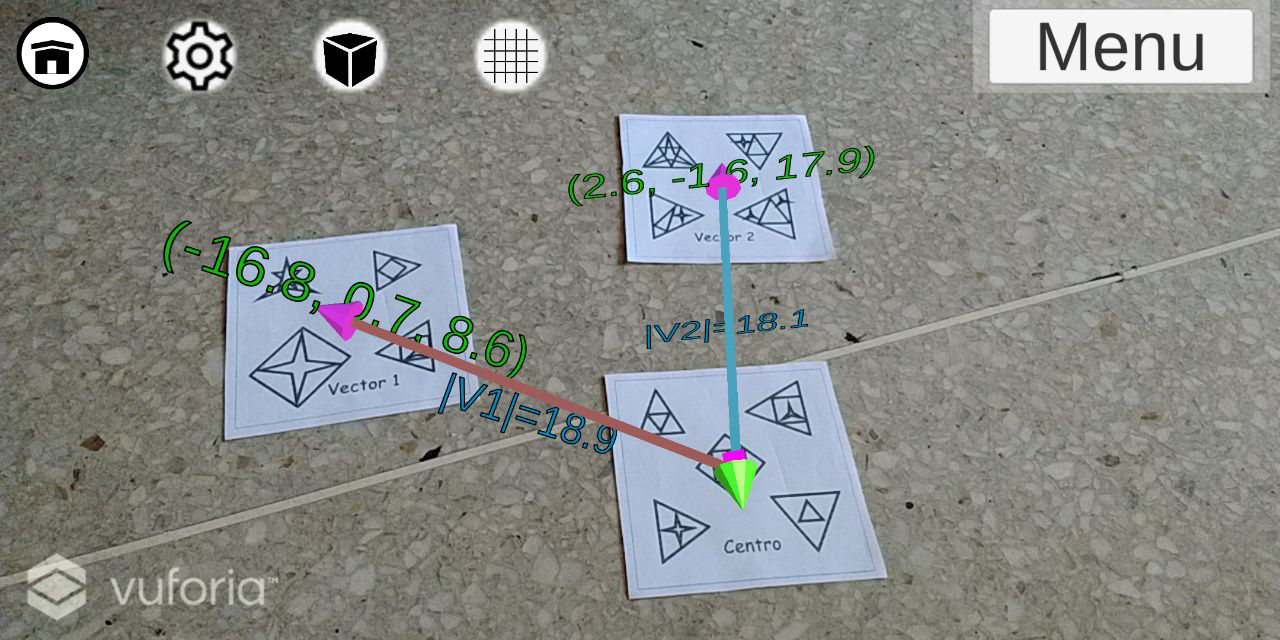
\includegraphics[width=0.5\textwidth]{figuras/vectores/Vectores1.png}
\caption{\label{fig:vec_ej1}Ejemplo de la aplicación de Vectores.}
\end{figure}
\FloatBarrier

\subsection{Image Render Target de Vuforia}
Para poder utilizar el motor de realidad aumentada de Vuforia, se generan tres \textit{Image Render Target}. Estos fueron utilizados como el centro donde comenzará cada uno de los vectores y los destinos del primer y segundo vector para controlar sus coordenadas. Para facilitar el reconocimiento por parte de Vuforia y minimizar las veces que los usuarios tengan que volver a apuntar las marcas con la cámara, se utilizaron figuras geométricas sencillas que apuntan en distintas direcciones con la finalidad de que el reconocedor de Vuforia tenga más información de la dirección de la imagen. 

En las Figuras \ref{fig:vec_centro} y \ref{fig:vec_vectores} se puede observar las marcas utilizadas, en estas se observa que se agregaron los nombres bajo ellas para facilitar su uso por los usuarios.

\begin{figure}[hbt!]
\centering
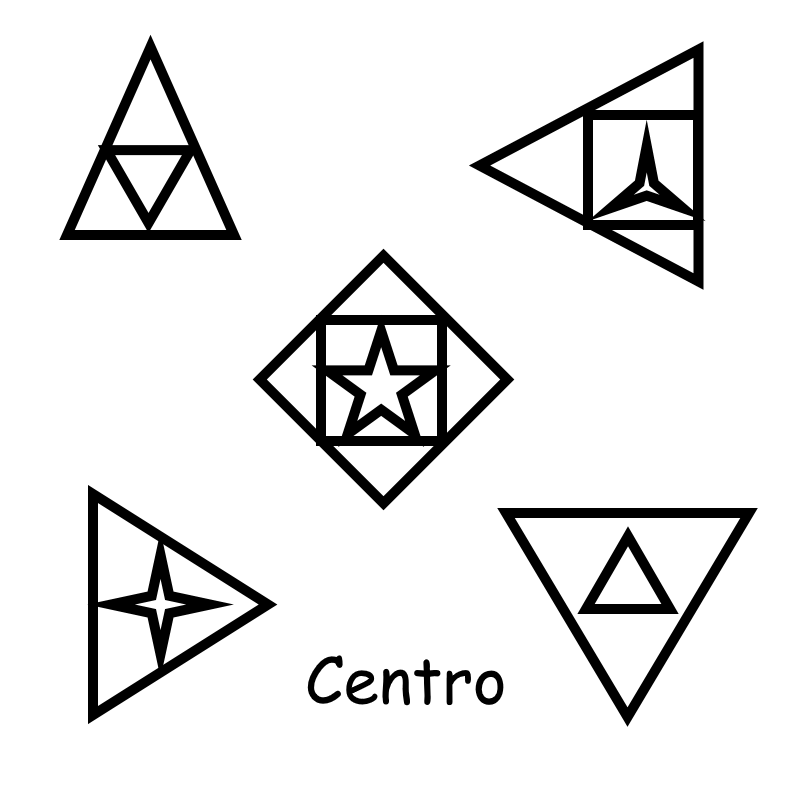
\includegraphics[width=0.5\textwidth]{figuras/vectores/ImageTarget1.png}
\caption{\label{fig:vec_centro}Marca de Centro para controlar el origen de los vectores.}
\end{figure}

\begin{figure}[hbt!]
\centering
\subfloat{\includegraphics[width=0.5\textwidth]{figuras/vectores/ImageTarget2.png}}
\subfloat{\includegraphics[width=0.5\textwidth]{figuras/vectores/ImageTarget3.png}}
\caption{\label{fig:vec_vectores}Marcas de Vector 1 y Vector 2 para controlar los destinos de los vectores.}
\end{figure}
\FloatBarrier

\subsection{Line Renderer}
Para representar los vectores gráficamente, se utilizó el componente \textit{Line Renderer} de Unity para el trazado de líneas y la simulación de los vectores a representar. Este componente es fácil de instanciar en la escena de la aplicación y de modificar, lo que permite que tanto los vectores, como los cálculos se realizan instantáneamente tanto al reconocer como al mover alguna de las marcas, lo que permite mayor agilidad y rapidez en el uso de la aplicación sin tener que esperar a que se vuelvan a calcular los datos. El principal problema que tiene este componente es que cada línea debe estar asociado a un \textit{GameObject} asociado, lo cual podría traer problemas de rendimiento si se instancian una gran cantidad de líneas en una escena. A pesar de esto, el proyecto no se vió afectado por esto ya que la mayor cantidad de líneas instanciadas a la vez, es igual a 16 (Figura \ref{fig:vec_linerenderer}), siendo la menor solo 2 al sólo representar los vectores.

\begin{figure}[hbt!]
\centering
\includegraphics[width=0.5\textwidth]{figuras/vectores/LineRenderer.png}
\caption{\label{fig:vec_linerenderer}Escena de Unity con las opciones “Suma”, “Ejes Dobles” y “Proyección Vector 2” activadas, la cual en total suma 16 \textit{Line Renderers} instanciados.}
\end{figure}
\FloatBarrier

\subsection{Scripts} 
Los \textit{Scripts} se pueden dividir en tres grupos distintos, correspondiente a sus funcionalidades, implementación general de vectores, operaciones de vectores y componentes adicionales.

\subsubsection{Implementación General de Vectores} 

\paragraph{Representación de Vectores}
Cada vector viene representado en la aplicación por dos \textit{GameObjects}, el primero que contiene un \textit{Line Renderer} para poder renderizar la longitud del vector, y el segundo que contiene el modelo de flecha que está en el destino de cada vector y representa la dirección del mismo. Ambos son controlados por el \textit{script} \textit{AnimateLine.cs} el cual se encarga de cada vector independientemente de revisar primero si las marcas de Centro y Vector están detectadas, y en ese caso instanciar la línea y flecha dirigidas hacia la marca destino (Figura \ref{fig:vec_representacion}).

\begin{figure}[hbt!]
\centering
\includegraphics[width=0.5\textwidth]{figuras/vectores/RepresentacionVectores.png}
\caption{\label{fig:vec_representacion}Representación de vectores con sus marcas en la aplicación.}
\end{figure}

Una vez ya instanciado el vector en la aplicación, si se detecta algún movimiento en la marca (se revisa en cada frame si se detectó o no un movimiento) se actualizará automáticamente la longitud y dirección del vector, afectando también los cálculos mostrados en la interfaz gráfica.
\FloatBarrier

\paragraph{Tracker}
El \textit{Tracker} (o rastreador) se encarga de conectar las ejecuciones necesarias en la representación de vectores con el reconocedor de marcas de Vuforia. Específicamente, el \textit{script} \textit{Tracker.cs} llama a las distintas funciones de los otros scripts. Al reconocer Centro con Vector 1, se encarga de llamar a la función de representación de vector, y de igual manera al reconocer Centro con Vector 2. Al reconocer las tres marcas a la vez, llama a las funciones de operaciones que pueden estar activadas para poder representarlas en la aplicación.

\paragraph{Interfaz Gráfica (Componentes X,Y,Z y Módulo del Vector)}
El manejo de la interfaz gráfica se divide en cuatro \textit{scripts}, los cuales son: \textit{TextDistance.cs}, el cual está encargado de colocar el texto de la distancia entre los vectores y el centro, además de las posiciones en el espacio de ambos vectores; \textit{PlaneHandler.cs}, el cual se encarga de activar y desactivar los planos de los ejes de forma rotativa; \textit{SettingsHandler.cs}, que se encarga de cambiar el modo de renderizar los ejes de forma rotativa entre no eje, completo con parte negativa, normales y doblemente largos; finalmente está \textit{BoxHandler.cs}, el cual maneja el renderizado una caja construida por las proyecciones del vector contra los ejes y rota entre renderizarlo para uno de los vectores.

\subsubsection{Operaciones de vectores}
Una vez detectada las marcas, el usuario podrá hacer uso del cálculo de las operaciones de vectores al presionar el botón “Menu”, las cuales se dividen en suma, resta, producto cruz, producto punto y limpiar. Todos los cálculos de las operaciones se realizan en el script Functions.cs el cual contiene las fórmulas necesarias para calcular cada una de ellas y mostrar gráficamente el resultado con el vector resultante (compuesto por su longitud y dirección). Por último, solo se puede mostrar una operación a la vez.

\paragraph{Suma}
La operación de suma entre los vectores $u=(u_x,u_y,u_z)$ y $v=(v_x,v_y,v_z)$ en un plano de tres dimensiones viene representada por la fórmula $u + v = (u_x+v_x, u_y+v_y, u_z+v_z)$.

En la siguiente figura (Figura \ref{fig:vec_suma}) se muestra un ejemplo de la operación sumar en funcionamiento.

\begin{figure}[hbt!]
\centering
\includegraphics[width=0.5\textwidth]{figuras/vectores/Suma.png}
\caption{\label{fig:vec_suma}Operación sumar en la aplicación.}
\end{figure}
\FloatBarrier

\paragraph{Resta}
La operación de resta entre los vectores $u=(u_x,u_y,u_z)$ y $v=(v_x,v_y,v_z)$ en un plano de tres dimensiones viene representada por la fórmula $u - v = (u_x-v_x, u_y-v_y, u_z-v_z)$.

En la siguiente figura (Figura \ref{fig:vec_resta}) se muestra un ejemplo de la operación restar en funcionamiento.

\begin{figure}[hbt!]
\centering
\includegraphics[width=0.5\textwidth]{figuras/vectores/Resta.png}
\caption{\label{fig:vec_resta}Operación restar en la aplicación.}
\end{figure}
\FloatBarrier

\paragraph{Producto Punto}
La operación de producto punto entre los vectores $u=(u_x,u_y,u_z)$ y $v=(v_x,v_y,v_z)$ en un plano de tres dimensiones viene representada por la fórmula $u . v = | u | | v | cos(u,v)$, en donde $| u | = \sqrt{u_x^2 + u_y^2 + u_z^2}$.

En la siguiente figura (Figura \ref{fig:vec_punto}) se muestra un ejemplo de la operación producto punto en funcionamiento.

\begin{figure}[hbt!]
\centering
\includegraphics[width=0.5\textwidth]{figuras/vectores/ProductoPunto.png}
\caption{\label{fig:vec_punto}Operación producto punto en la aplicación.}
\end{figure}
\FloatBarrier

\paragraph{Producto Cruz}
La operación de producto cruz entre los vectores $u=(u_x,u_y,u_z)$ y $v=(v_x,v_y,v_z)$ en un plano de tres dimensiones viene representada por la fórmula $u \times v = (u_y*v_z - u_z*v_y, u_z*v_x - u_x*v_z, u_x*v_y - v_y*v_x)$.

En la siguiente figura (Figura \ref{fig:vec_cruz}) se muestra un ejemplo de la operación producto cruz en funcionamiento.

\begin{figure}[hbt!]
\centering
\includegraphics[width=0.5\textwidth]{figuras/vectores/ProductoCruz.png}
\caption{\label{fig:vec_cruz}Operación producto cruz en la aplicación.}
\end{figure}
\FloatBarrier

\paragraph{Limpiar}

La operación Limpiar se encarga de desactivar la función previamente activada y mostrar únicamente la interfaz original con la representación de los dos vectores.

\subsubsection{Componentes adicionales}
Por último, aparte de las operaciones de vectores en la interfaz gráfica, se encuentran cuatro botones: volver al menú principal, cambiar ejes, proyección de vectores y planos en el origen. Estas opciones se pueden activar independientes a las operaciones, es decir, no tienen restricciones entre ellas y se pueden ver todas activadas al mismo tiempo.

\paragraph{Ejes del origen}
El botón de ejes en el origen, permite al usuario colocar distintos tipos de ejes en las coordenadas $(x,y,z)$ para facilitar la visualización del plano cartesiano. Estas operaciones son calculadas en el \textit{script} \textit{AnimateLineAxis.cs} que se encarga únicamente de instanciar cada uno de los ejes con su dirección determinada.  Las distintas opciones que se encuentran son:

\begin{enumerate}
    \item Desactivado.
    \item Ejes positivos.
    \item Ejes positivos y negativos (Figura \ref{fig:vec_opcion_ejes}).
    \item Ejes positivos extendidos.
\end{enumerate}

\begin{figure}[hbt!]
\centering
\includegraphics[width=0.5\textwidth]{figuras/vectores/Ejes.png}
\caption{\label{fig:vec_opcion_ejes}Opción de ejes positivos y negativos activada en la aplicación.}
\end{figure}
\FloatBarrier

\paragraph{Proyección del Vector}
El botón de proyección de vectores permite representar la proyección de uno de los dos vectores de acuerdo a su origen y destino. Dependiendo de cuál vector se encuentre activado, además cambia el color del botón (verde para Vector 1 y azul para Vector 2). Estas operaciones se realizan en el \textit{script} \textit{AnimateAxis.cs} asociado a cada vector, y se encarga de instanciar cada una de las líneas para finalmente proyectar el vector, representado en el plano de tres dimensiones como un cubo. Las distintas opciones que se encuentran son:

\begin{enumerate}
    \item Desactivado.
    \item Proyección del Vector 1 (Figura \ref{fig:vec_opcion_proyeccion}).
    \item Proyección del Vector 2.
\end{enumerate}

\begin{figure}[hbt!]
\centering
\includegraphics[width=0.5\textwidth]{figuras/vectores/Proyeccion.png}
\caption{\label{fig:vec_opcion_proyeccion}Opción de proyección del Vector 1 activada.}
\end{figure}
\FloatBarrier

\paragraph{Planos en el Origen}
El botón de planos en el origen permite al usuario instanciar en la escena un plano cartesiano que facilita las mediciones de los vectores. Cada plano tiene una medida de $30\times 30$ cuadrículas, cada una de aproximadamente $1\times 1cm$ reales. Estos planos se instancian en el \textit{script} \textit{AnimateLineAxis.cs}. Las distintas opciones que se encuentran disponibles son:

\begin{enumerate}
    \item Desactivado.
    \item Plano en el eje x (Figura \ref{fig:vec_opcion_planos_x}).
    \item Plano en el eje y.
    \item Plano en el eje z.
    \item Planos en los ejes x,y,z (Figura \ref{fig:vec_opcion_planos_xyz}).
\end{enumerate}

\begin{figure}[hbt!]
\centering
\includegraphics[width=0.5\textwidth]{figuras/vectores/Planos1.png}
\caption{\label{fig:vec_opcion_planos_x}Opción de plano en el eje x activada.}
\end{figure}

\begin{figure}[hbt!]
\centering
\includegraphics[width=0.5\textwidth]{figuras/vectores/Planos2.png}
\caption{\label{fig:vec_opcion_planos_xyz}Opción de planos en los ejes x,y,z activada.}
\end{figure}
\FloatBarrier

\subsection{Consideraciones Importantes al Momento de Realizar Operaciones} 
En el editor de escenas de Unity, las unidades al momento de ser calculadas están definidas en Unidades de Vuforia, a diferencia de una unidad utilizada en la vida real como centímetros o pulgadas. Uno de los retos del proyecto fue encontrar cual era la relación entre unidades de Vuforia y centímetros para que los vectores tengan las mismas mediciones al ser utilizadas por la aplicación en la vida real. Luego de realizar varias pruebas, se encontró que utilizando marcas de detección de $10\times 10cm$, se encuentra que la relación entre unidades de Vuforia y centímetros es de $1:1$, es decir son totalmente equivalentes. Esto permite que la representación de los vectores tengan a lo sumo un margen de error de $1 cm$ al momento de ser calculados por Vuforia y la aplicación.


\section{VisualizAR: Gráficas}
Esta sección de la aplicación se busca presentar los conceptos de gráficas a estudiantes de bachillerato, mediante la presentación interactiva de distintas funciones parametrizables con dos coordenadas, las cuales son manifestadas en 3D mediante el uso de la realidad aumentada. Además, se utiliza al tiempo como un tercer parámetro, para aumentar el llamativo de las gráficas. En las Figuras \ref{fig:graf_ej1}, \ref{fig:graf_ej2} y \ref{fig:graf_ej3} se pueden observar ejemplos de esta aplicación.

Para realizar esto se utilizaron dos \textit{Image Render Target} de Vuforia, uno como base y otro como menú; un \textit{Shader} para la coloración de la gráfica y cuatro \textit{Scripts} de control.

\begin{figure}[hbt!]
\centering
\includegraphics[width=0.5\textwidth]{figuras/graficas/ej1.png}
\caption{\label{fig:graf_ej1}Ejemplo de la aplicación de Gráficas.}
\end{figure}

\begin{figure}[hbt!]
\centering
\includegraphics[width=0.5\textwidth]{figuras/graficas/ej2.png}
\caption{\label{fig:graf_ej2}Ejemplo de la aplicación de Gráficas.}
\end{figure}

\begin{figure}[hbt!]
\centering
\includegraphics[width=0.5\textwidth]{figuras/graficas/ej3.png}
\caption{\label{fig:graf_ej3}Ejemplo de la aplicación de Gráficas.}
\end{figure}
\FloatBarrier

\subsection{Image Render Target de Vuforia}
Para poder utilizar el motor de realidad aumentada de Vuforia, se generaron dos \textit{Image Render Target}. Estos fueron utilizados como la base donde poder mostrar las gráficas y los botones para controlar la selección de qué función visualizar.

En las Figuras \ref{fig:graf_botones} y \ref{fig:graf_centro} se puede observar las marcas utilizadas, en estas se observa que se agregaron los nombres bajo ellas para facilitar su uso por los usuarios.

\begin{figure}[hbt!]
\centering
\includegraphics[width=0.4\textwidth]{figuras/graficas/botones.png}
\caption{\label{fig:graf_botones}Marca de Botones para controlar la aplicación.}
\end{figure}

\begin{figure}[hbt!]
\centering
\includegraphics[width=0.4\textwidth]{figuras/graficas/centro.png}
\caption{\label{fig:graf_centro}Marca de Gráficas para controlar la posición donde visualizar las funciones.}
\end{figure}
\FloatBarrier

\subsection{Shader}
Para aumentar el llamativo visual de las gráficas, se creó un \textit{Shader} para controlar la forma de colorear. Este se basa en mostrar la representación del espacio vectorial, centrado en base, en el espacio de colores RGB. Esto se realiza mediante la normalización del espacio, utilizando un factor de escalamiento, para pasar al espacio $[-1,1]\times[-1,1]\times[-1,1]$ y luego transformarlo al espacio $[0,1]\times[0,1]\times[0,1]$, el cual es representable como un color RGB. El código se puede encontrar en la carpeta de \textit{Shaders} bajo el nombre \textit{ColoredPoint.shader}. En la Figura \ref{fig:graf_shader} se observa un ejemplo de la coloración generada por el \textit{Shader}.

\begin{figure}[hbt!]
\centering
\includegraphics[width=0.5\textwidth]{figuras/graficas/shader.png}
\caption{\label{fig:graf_shader}Ejemplo de la visualización del espacio vectorial mediante colores RGB.}
\end{figure}
\FloatBarrier

\subsection{Scripts}
Los \textit{Scripts} se pueden dividir en dos grupos, los que manejan las gráficas y el que maneja la interfaz.

\subsubsection{Manejo de Gráficas} 
El proceso de graficar se realiza mediante la parametrización de superficies. En el caso de la aplicación, se parametrizan superficies 3D mediante coordenadas 2D del espacio $[0,1]\times[0,1]$, conocido en inglés como U V Mapping, el cual consiste en proyectar un plano 2D a una superficie 3D. Además, se incluye un parámetro de tiempo para darle un aspecto dinámico a las gráficas para atraer la atención del usuario. El desarrollo del manejador de gráficas se basó en las explicaciones de Jasper Flick \cite{flick2017}, adaptado a los requerimientos específicos de la aplicación y con más funciones.

Las funciones utilizadas en la aplicación para generar las superficies visualizadas tienen la forma presentada en la Ecuación \ref{eq:graf_func}, es importante destacar que no siempre tienen que usar los tres parámetros de entrada.

\begin{equation}\label{eq:graf_func}
\begin{aligned}
    & [0,1]\times[0,1]\times\mathbb{R}^+ \rightarrow \mathbb{R}^3 \\
    & f(u,v,t) = (x,y,z)
\end{aligned}
\end{equation}

Para representar los puntos de la superficie, se utilizó una malla 2D de $100 \times 100$ cubos (para darles un tamaño visible por los usuarios), la cual se instancia al comienzo de la aplicación de gráficas y  se adapta dinámicamente a la función que se desea graficar. Un ejemplo para visualizar los cubos que forman la superficie, es la gráfica del círculo de la Figura \ref{fig:graf_malla}. 

\begin{figure}[hbt!]
\centering
\includegraphics[width=0.5\textwidth]{figuras/graficas/malla.png}
\caption{\label{fig:graf_malla}Gráfica del círculo donde se observan los cubos que forman la malla.}
\end{figure}

Todo esto es manejado por el \textit{Script} \textit{Graph.cs}, el cual, además, controla las funciones para graficar. Para facilitar desarrollo y la futura posible expansión, se agregaron: \textit{GraphFunction.cs} el cual contiene el prototipo de las funciones que se grafican, para poder crear y utilizar más funciones; y \textit{GraphFunctionName.cs} el cual contiene un enumerable de los nombres de las funciones, para poder visualizarlas mejor en los menús dentro del editor de Unity.
\FloatBarrier

\subsubsection{Calculadora}
La calculadora se encarga de darle el control al usuario de decidir cuál gráfica mostrar al presionar cada uno de los botones sin necesidad de tener estas opciones en la interfaz gráfica. Por facilidad, se decidió tener tres páginas diferentes de opciones de ocho botones cada uno (identificados con una letra), las cuales pueden ser presionadas, emitiendo un sonido y animacion; e inmediatamente cambiar la gráfica actual. Aparte, la calculadora muestra una pequeña pantalla transparente la cual contiene el nombre de la gráfica actual. En la Figura \ref{fig:graf_calculadora} se puede observar la calculadora como se ve en la aplicación.

\begin{figure}[hbt!]
\centering
\includegraphics[width=0.5\textwidth]{figuras/graficas/calculadora.png}
\caption{\label{fig:graf_calculadora}Calculadora como se ve en la aplicación.}
\end{figure}

Todos los procedimientos y funciones de la calculadora están calculados en \textit{ARsound.cs} la cual se encarga de:
\begin{enumerate}
	\item Inicializar la calculadora con la primera página y primera función, Seno y conectarla con el Manejador de Funciones.
	\item Detectar cuando el usuario ha presionado alguno de los botones de gráficas, para emitir una animación de presionado de botón, un sonido y cambiar tanto la gráfica en el Manejador de Funciones como la pantalla de la calculadora con el nombre correspondiente. Cabe resaltar que la pequeña animación es realizada a partir de script y no con el animador de Unity.
	\item Detectar cuando el usuario ha presionado alguno de los cambios de página para actualizar la interfaz de la calculadora. En caso de que el usuario presione un cambio de página incorrecto (por ejemplo, estar en la primera página y presionar el botón “atrás”) se emite un sonido de error diferente al sonido predeterminado.
\end{enumerate}

\FloatBarrier

\subsubsection{Funciones} 
La aplicación consta de veinticuatro funciones para graficar, estas son explicadas a continuación.

\paragraph{Seno}
Dado por la ecuación $f(u,v,t)=(u,Sen(\pi * (u + t)),v)$. La Figura \ref{fig:graf_seno} es la gráfica de esta función, la cual es la opción A del menú.

\begin{figure}[hbt!]
\centering
\includegraphics[width=0.5\textwidth]{figuras/graficas/seno.png}
\caption{\label{fig:graf_seno}Gráfica de la función Seno.}
\end{figure}
\FloatBarrier

\paragraph{Seno 2D}
Dado por la ecuación $f(u,v,t)=(u,Sen(\pi * (u + v+ t))*0.5,v)$. La Figura \ref{fig:graf_seno2d} es la gráfica de esta función, la cual es la opción B del menú.

\begin{figure}[hbt!]
\centering
\includegraphics[width=0.5\textwidth]{figuras/graficas/seno2d.png}
\caption{\label{fig:graf_seno2d}Gráfica de la función Seno 2D.}
\end{figure}
\FloatBarrier

\paragraph{Media del Seno}
Dado por la ecuación $f(u,v,t)=(u,Sen(\pi * (u + t))/2+Sen(\pi * (v+ t))/2,v)$. La Figura \ref{fig:graf_media_seno} es la gráfica de esta función, la cual es la opción C del menú.

\begin{figure}[hbt!]
\centering
\includegraphics[width=0.5\textwidth]{figuras/graficas/media_seno.png}
\caption{\label{fig:graf_media_seno}Gráfica de la función Media del Seno.}
\end{figure}
\FloatBarrier

\paragraph{Multiseno}
Dado por la ecuación $f(u,v,t)=(u,Sen(\pi * (u + t))*2/3+Sen(2 * \pi * (v + 2 * t))/3,v)$. La Figura \ref{fig:graf_multiseno} es la gráfica de esta función, la cual es la opción D del menú.

\begin{figure}[hbt!]
\centering
\includegraphics[width=0.5\textwidth]{figuras/graficas/multiseno.png}
\caption{\label{fig:graf_multiseno}Gráfica de la función Mutiseno.}
\end{figure}
\FloatBarrier

\paragraph{Multiseno 2D}
Dado por la ecuación $f(u,v,t)=(u, (4 * Sen(\pi * (u + v + t / 2)) + Sen(\pi * (u + t)) + Sen(2 * \pi * (v + 2 * t)) * 0.5) * 1 / 5.5,v)$. La Figura \ref{fig:graf_multiseno2d} es la gráfica de esta función, la cual es la opción E del menú.

\begin{figure}[hbt!]
\centering
\includegraphics[width=0.5\textwidth]{figuras/graficas/multiseno2d.png}
\caption{\label{fig:graf_multiseno2d}Gráfica de la función Mutiseno 2D.}
\end{figure}
\FloatBarrier

\paragraph{Onda}
Dado por la ecuación $f(u,v,t)=(u, Sen(\pi * (4 * d - t))/(1 + 10 * d),v)$ donde $d=\sqrt{u * u + v * v}$. La Figura \ref{fig:graf_onda} es la gráfica de esta función, la cual es la opción F del menú.

\begin{figure}[hbt!]
\centering
\includegraphics[width=0.5\textwidth]{figuras/graficas/onda.png}
\caption{\label{fig:graf_onda}Gráfica de la función Onda.}
\end{figure}
\FloatBarrier

\paragraph{Círculo}
Dado por la ecuación $f(u,v,t)=(Sen(\pi * u), 0,Cos(\pi * u))$. La Figura \ref{fig:graf_circulo} es la gráfica de esta función, la cual es la opción G del menú.

\begin{figure}[hbt!]
\centering
\includegraphics[width=0.5\textwidth]{figuras/graficas/circulo.png}
\caption{\label{fig:graf_circulo}Gráfica de la función Círculo.}
\end{figure}
\FloatBarrier

\paragraph{Remolino}
Dado por la ecuación $f(u,v,t)=(Sen(\pi * w), u, Cos(\pi * w))$ donde $w = u + t$. La Figura \ref{fig:graf_remolino} es la gráfica de esta función, la cual es la opción H del menú.

\begin{figure}[hbt!]
\centering
\includegraphics[width=0.5\textwidth]{figuras/graficas/remolino.png}
\caption{\label{fig:graf_remolino}Gráfica de la función Remolino.}
\end{figure}
\FloatBarrier

\paragraph{Cilindro}
Dado por la ecuación $f(u,v,t)=(r*Sen(\pi * u), v, r*Cos(\pi * u))$ donde $r = 1$. La Figura \ref{fig:graf_cilindro} es la gráfica de esta función, la cual es la opción I del menú.

\begin{figure}[hbt!]
\centering
\includegraphics[width=0.5\textwidth]{figuras/graficas/cilindro.png}
\caption{\label{fig:graf_cilindro}Gráfica de la función Cilindro.}
\end{figure}
\FloatBarrier

\paragraph{Cilindro Tambaleante}
Dado por la ecuación $f(u,v,t)=(r*Sen(\pi * u), v, r*Cos(\pi * u))$ donde $r = 1 + Sen(6 * pi * u) * 0.2$. La Figura \ref{fig:graf_cilindro_tambaleante} es la gráfica de esta función, la cual es la opción J del menú.

\begin{figure}[hbt!]
\centering
\includegraphics[width=0.5\textwidth]{figuras/graficas/cilindro_tambaleante.png}
\caption{\label{fig:graf_cilindro_tambaleante}Gráfica de la función Cilindro Tambaleante.}
\end{figure}
\FloatBarrier

\paragraph{Cilindro de Olla}
Dado por la ecuación $f(u,v,t)=(r*Sen(\pi * u), v, r*Cos(\pi * u))$ donde $r = 1 + Sen(2 * pi * v) * 0.2$. La Figura \ref{fig:graf_cilindro_olla} es la gráfica de esta función, la cual es la opción K del menú.

\begin{figure}[hbt!]
\centering
\includegraphics[width=0.5\textwidth]{figuras/graficas/cilindro_olla.png}
\caption{\label{fig:graf_cilindro_olla}Gráfica de la función Cilindro de Olla.}
\end{figure}
\FloatBarrier

\paragraph{Cilindro de Torsión}
Dado por la ecuación $f(u,v,t)=(r*Sen(\pi * u), v, r*Cos(\pi * u))$ donde $r = 0.8 + Sen(\pi * (6 * u + 2 * v + t)) * 0.2$. La Figura \ref{fig:graf_cilindro_torsion} es la gráfica de esta función, la cual es la opción L del menú.

\begin{figure}[hbt!]
\centering
\includegraphics[width=0.5\textwidth]{figuras/graficas/cilindro_torsion.png}
\caption{\label{fig:graf_cilindro_torsion}Gráfica de la función Cilindro de Torsión.}
\end{figure}
\FloatBarrier

\paragraph{Esfera}
Dado por la ecuación $f(u,v,t)=(r*Sen(\pi * u), Sen(\pi * 0.5 * v), r*Cos(\pi * u))$ donde $r = Cos(\pi * 0.5 * v)$. La Figura \ref{fig:graf_esfera} es la gráfica de esta función, la cual es la opción M del menú.

\begin{figure}[hbt!]
\centering
\includegraphics[width=0.5\textwidth]{figuras/graficas/esfera.png}
\caption{\label{fig:graf_esfera}Gráfica de la función Esfera.}
\end{figure}
\FloatBarrier

\paragraph{Esfera Cardioide}
Dado por la ecuación $f(u,v,t)=(r*Sen(\pi * u), v, r*Cos(\pi * u))$ donde $r = Cos(\pi * 0.5 * v)$. La Figura \ref{fig:graf_esfera_cardioide} es la gráfica de esta función, la cual es la opción N del menú.

\begin{figure}[hbt!]
\centering
\includegraphics[width=0.5\textwidth]{figuras/graficas/esfera_cardioide.png}
\caption{\label{fig:graf_esfera_cardioide}Gráfica de la función Esfera Cardioide.}
\end{figure}
\FloatBarrier

\paragraph{Esfera Pulsante}
Dado por la ecuación $f(u,v,t)=(s*Sen(\pi * u), r * Sen(\pi * 0.5 * v), s*Cos(\pi * u))$ donde $s = r*Cos(\pi * 0.5 * v)$ y $r=0.8 + Sen(\pi * (6 * u + t)) * 0.1 + Sen(\pi * (4 * v + t)) * 0.1$. La Figura \ref{fig:graf_esfera_pulsante} es la gráfica de esta función, la cual es la opción O del menú.

\begin{figure}[hbt!]
\centering
\includegraphics[width=0.5\textwidth]{figuras/graficas/esfera_pulsante.png}
\caption{\label{fig:graf_esfera_pulsante}Gráfica de la función Esfera Pulsante.}
\end{figure}
\FloatBarrier

\paragraph{Toroide Exterior}
Dado por la ecuación $f(u,v,t)=(s*Sen(\pi * u), Sen(\pi * 0.5 * v), s*Cos(\pi * u))$ donde $s = Cos(\pi * 0.5 * v) + 0.5$. La Figura \ref{fig:graf_toroide_exterior} es la gráfica de esta función, la cual es la opción P del menú.

\begin{figure}[hbt!]
\centering
\includegraphics[width=0.5\textwidth]{figuras/graficas/toroide_exterior.png}
\caption{\label{fig:graf_toroide_exterior}Gráfica de la función Toroide Exterior.}
\end{figure}
\FloatBarrier

\paragraph{Toroide de Intersección}
Dado por la ecuación $f(u,v,t)=(s*Sen(\pi * u), Sen(\pi *  v), s*Cos(\pi * u))$ donde $s = Cos(\pi * 0.5 * v) + 0.5$. La Figura \ref{fig:graf_toroide_interseccion} es la gráfica de esta función, la cual es la opción Q del menú.

\begin{figure}[hbt!]
\centering
\includegraphics[width=0.5\textwidth]{figuras/graficas/toroide_interseccion.png}
\caption{\label{fig:graf_toroide_interseccion}Gráfica de la función Toroide de Intersección.}
\end{figure}
\FloatBarrier

\paragraph{Toroide de Cuerno}
Dado por la ecuación $f(u,v,t)=(s*Sen(\pi * u), Sen(\pi *  v), s*Cos(\pi * u))$ donde $s = Cos(\pi * v)+r_1$ y $r_1 = 1$. La Figura \ref{fig:graf_toroide_cuerno} es la gráfica de esta función, la cual es la opción R del menú.

\begin{figure}[hbt!]
\centering
\includegraphics[width=0.5\textwidth]{figuras/graficas/toroide_cuerno.png}
\caption{\label{fig:graf_toroide_cuerno}Gráfica de la función Toroide de Cuerno.}
\end{figure}
\FloatBarrier

\paragraph{Toroide Anidado}
Dado por la ecuación $f(u,v,t)=(s*Sen(\pi * u), r_2 * Sen(\pi *  v), s*Cos(\pi * u))$ donde $s = Cos(\pi * v)$, $r_1 = 1$ y $r_2 = 0.5$. La Figura \ref{fig:graf_toroide_anidado} es la gráfica de esta función, la cual es la opción S del menú.

\begin{figure}[hbt!]
\centering
\includegraphics[width=0.5\textwidth]{figuras/graficas/toroide_anidado.png}
\caption{\label{fig:graf_toroide_anidado}Gráfica de la función Toroide Anidado.}
\end{figure}
\FloatBarrier

\paragraph{Toroide Estrella}
Dado por la ecuación $f(u,v,t)=(s*Sen(\pi * u), r_2 * Sen(\pi *  v), s*Cos(\pi * u))$ donde $s = Cos(\pi * v)$, $r_1 = 10.65 + Sen(\pi * (6 * u + t)) * 0.1$ y $r_2 = 0.2 + Sen(\pi * (4 * v + t)) * 0.05$. La Figura \ref{fig:graf_toroide_estrella} es la gráfica de esta función, la cual es la opción T del menú.

\begin{figure}[hbt!]
\centering
\includegraphics[width=0.5\textwidth]{figuras/graficas/toroide_estrella.png}
\caption{\label{fig:graf_toroide_estrella}Gráfica de la función Toroide Estrella.}
\end{figure}
\FloatBarrier

\paragraph{Banda de Mobius}
Dado por la ecuación $f(u,v,t)=(te*Cos(nu),te*Sen(nu),halfnv*Sen(halfnu))$ donde $te = 1 + halfnv * Cos(halfnu)$, $nu = 2 * halfnu$, $halfnv = v - 0.5$ y $halfnu = (u + t * 0.05) * \pi$ . La Figura \ref{fig:graf_mobius} es la gráfica de esta función, la cual es la opción U del menú.

\begin{figure}[hbt!]
\centering
\includegraphics[width=0.5\textwidth]{figuras/graficas/mobius.png}
\caption{\label{fig:graf_mobius}Gráfica de la función Banda de Mobius.}
\end{figure}
\FloatBarrier

\paragraph{Banda Especial de Mobius}
Dado por la ecuación $f(u,v,t)=(te*Cos(nu),te*Sen(nu),halfnv*Sen(halfnu))$ donde $te = 1 + halfnv * Cos(halfnu)$, $nu = 2 * halfnu$, $halfnv = (v - 0.5) * Cos(\pi * (t * 0.05 + v)) * Cos(\pi * (t * 0.1f + u)) * Cos(\pi * (t * 0.2 + u + v))$ y $halfnu = (u + t * 0.05) * \pi$ . La Figura \ref{fig:graf_mobius_especial} es la gráfica de esta función, la cual es la opción V del menú.

\begin{figure}[hbt!]
\centering
\includegraphics[width=0.5\textwidth]{figuras/graficas/mobius_especial.png}
\caption{\label{fig:graf_mobius_especial}Gráfica de la función Banda Especial de Mobius.}
\end{figure}
\FloatBarrier

\paragraph{Botella de Klein Estática}
Dado por la ecuación $f(u,v,t)=(-2/15 * cu * (3 * cv - 30 * su + 90 * cu^4 * su - 60 * cu^6 * su + 5 * cu * cv * su), -1/15 * su * (3 * cv - 3 * cu^2 * cv - 48 * cu^4 * cv + 48 * cu^6 * cv - 60 * su + 5 * cu * cv * su - 5 * cu^3 * cv * su - 80 * cu^5 * cv * sv + 80 * cu^7 * cv * su) -2, 2/15 * (3 + 5 * cu * su) * sv)$ donde $sv = Sen(nv)$, $cv = Cos(nv)$, $su = Sen(nu)$, $cu = Cos(nu)$, $nv = v * \pi * 2$ y $nu = u * \pi$. La Figura \ref{fig:graf_klein_estatico} es la gráfica de esta función, la cual es la opción W del menú.

\begin{figure}[hbt!]
\centering
\includegraphics[width=0.5\textwidth]{figuras/graficas/klein_estatico.png}
\caption{\label{fig:graf_klein_estatico}Gráfica de la función Botella de Klein Estática.}
\end{figure}
\FloatBarrier

\paragraph{Botella de Klein Dinámica}
Dado por la ecuación $f(u,v,t)=(-2/15 * cu * (3 * cv - 30 * su + 90 * cu^4 * su - 60 * cu^6 * su + 5 * cu * cv * su), -1/15 * su * (3 * cv - 3 * cu^2 * cv - 48 * cu^4 * cv + 48 * cu^6 * cv - 60 * su + 5 * cu * cv * su - 5 * cu^3 * cv * su - 80 * cu^5 * cv * sv + 80 * cu^7 * cv * su) -2, 2/15 * (3 + 5 * cu * su) * sv)$ donde $sv = Sen(nv)$, $cv = Cos(nv)$, $su = Sen(nu)$, $cu = Cos(nu)$, $nv = (v+ t * 0.2) * \pi * 2$ y $nu = (u+ t * 0.05) * \pi$. La Figura \ref{fig:graf_klein_dinamico} es la gráfica de esta función, la cual es la opción X del menú.

\begin{figure}[hbt!]
\centering
\includegraphics[width=0.5\textwidth]{figuras/graficas/klein_dinamico.png}
\caption{\label{fig:graf_klein_dinamico}Gráfica de la función Botella de Klein Dinámica.}
\end{figure}
\FloatBarrier

\bibliographystyle{plain}
\bibliography{references}
\end{document} to your LaTeX file where you want your
% title page.
%
%%%%%%%%%%%%%%%%%%%%%%%%%%%%%%%%%%%%%%%%%
%\title{Title page with logo}
%----------------------------------------------------------------------------------------
%	PACKAGES AND OTHER DOCUMENT CONFIGURATIONS
%----------------------------------------------------------------------------------------

\documentclass[12pt]{report}
\setcounter{tocdepth}{4}
\setcounter{secnumdepth}{4}
\usepackage[spanish]{babel}
\usepackage[utf8]{inputenc}
\usepackage{amsmath}
\usepackage{graphicx}
\usepackage[colorinlistoftodos]{todonotes}
\usepackage{hyperref}
\usepackage{acronym}
\usepackage{fancyhdr}
\usepackage{placeins}
\usepackage{amssymb}
\usepackage{etoolbox}
\usepackage{subfig}

\addto\captionsspanish{% Replace "english" with the language you use
  \renewcommand{\contentsname}%
    {Índice General}%
  \renewcommand{\listfigurename}%
    {Índice de Figuras}%
  \renewcommand{\listtablename}%
    {Índice de Tablas}%
  \renewcommand{\bibname}%
    {Referencias}%
  \renewcommand{\thechapter}{\Roman{chapter}}
  \renewcommand{\thesection}{\arabic{chapter}.\arabic{section}}
  \renewcommand{\thefigure}{\arabic{chapter}.\arabic{figure}}
  \renewcommand{\theequation}{\arabic{chapter}.\arabic{equation}}
}

\makeatletter
\def\@makechapterhead#1{%
  %%%%\vspace*{50\p@}% %%% removed!
  {\parindent \z@ \centering \normalfont
    \ifnum \c@secnumdepth >\m@ne
        \LARGE\bfseries \MakeUppercase{\@chapapp}\space \thechapter % <--- uppercase
        \par\nobreak
        \vskip 0\p@
    \fi
    \interlinepenalty\@M
    \Large \bfseries \MakeUppercase{#1}\par\nobreak
    \vskip 30\p@
  }}
\def\@makeschapterhead#1{%
  %%%%%\vspace*{50\p@}% %%% removed!
  {\parindent \z@ \centering
    \normalfont
    \interlinepenalty\@M
    \Large \bfseries  \MakeUppercase{#1}\par\nobreak
    \vskip 30\p@
  }}
\makeatother

\pagestyle{fancy}
\fancyhf{}
\fancyheadoffset{0cm}
\renewcommand{\headrulewidth}{0pt} 
\renewcommand{\footrulewidth}{0pt}
\fancyhead[R]{\thepage}
\fancypagestyle{plain}{%
   \fancyhf{}%
   \fancyhead[R]{\thepage}%
}

\fancypagestyle{chapterstart}{%
  \renewcommand{\headrulewidth}{0pt}%
  \fancyhf{}%
}

% \patchcmd{\chapter}{plain}{chapterstart}{}{}


\begin{document}

\begin{titlepage}

\newcommand{\HRule}{\rule{\linewidth}{0.5mm}} % Defines a new command for the horizontal lines, change thickness here



\center % Center everything on the page
 
%----------------------------------------------------------------------------------------
%	HEADING SECTIONS
%----------------------------------------------------------------------------------------
\includegraphics[width=0.15\textwidth]{figuras/logo_usb.png}\\[0.3cm]
\textsc{\bfseries UNIVERSIDAD SIMÓN BOLÍVAR}\\
\textsc{\bfseries DECANATO DE ESTUDIOS PROFESIONALES}\\
\textsc{\bfseries COORDINACIÓN DE INGENIERÍA DE COMPUTACIÓN}\\[4cm] % Name of your university/college

%----------------------------------------------------------------------------------------
%	TITLE SECTION
%----------------------------------------------------------------------------------------


{ \LARGE \bfseries VisualizAR}\\[3cm] % Title of your document
 
%----------------------------------------------------------------------------------------
%	AUTHOR SECTION
%----------------------------------------------------------------------------------------

% If you don't want a supervisor, uncomment the two lines below and remove the section above
\normalfont Por\\[0.3cm]
Christian Oliveros 13-11000\\% Your name
Alexander Romero 13-11274\\[2cm] % Your name

Realizado con la asesoria de:\\
Angela Di Serio\\[1cm]

EP-4793 Mini Proyecto de Desarrollo de Software\\[1cm]

%----------------------------------------------------------------------------------------
%	DATE SECTION
%----------------------------------------------------------------------------------------

{\bfseries Sartenejas, \today}\\[2cm] % Date, change the \today to a set date if you want to be precise

%----------------------------------------------------------------------------------------
%	LOGO SECTION
%----------------------------------------------------------------------------------------

 % Include a department/university logo - this will require the graphicx package
 
%----------------------------------------------------------------------------------------

\vfill % Fill the rest of the page with whitespace

\end{titlepage}

\pagenumbering{roman}
%\begin{abstract}
%Your abstract. \ac{API}
%
%\ac{API}
%\end{abstract}

\tableofcontents
\listoffigures
%\listoftables

\chapter*{Lista de Acrónimos}
\begin{acronym}
	\acro{USB}[USB]{Universidad Sim\'on Bol\'ivar}
	\acro{DEP}[DEP]{Decanato de Estudios Profesionales}
	\acro{PDF}[PDF]{\textit{Portable Document Format}, Documento en Formato Portable\copyright}
	\acro{3D}[3D]{\textit{Three Dimensions}, Tres Dimensiones}
	\acro{API}[API]{\textit{Application Programming Interface}, Interfaz de Programación de Aplicaciones}
	\acro{RGB}[RGB]{\textit{Red Green Blue}, Rojo Verde Azul}
	\acro{AR}[AR]{\textit{Augmented Reality}, Realidad Aumentada}
	\acro{MB}[MB]{\textit{Mega Byte}}
	\acro{cm}[cm]{Centímetro}
	\acro{GPU}[GPU]{\textit{Graphics Processing Unit}, Unidad de Procesamiento Gráfico}
	\acro{SDK}[SDK]{\textit{Software Development Kit}, Kit de Desarrollo de Software}
	\acro{AR/RA}[AR/RA]{\textit{Augmented Reality}, Realidad Aumentada}
	\acro{VR}[VR]{\textit{Virtual Reality}, Realidad Virtual}

\end{acronym}
\cleardoublepage
\pagenumbering{arabic}
\clearpage

\makeatletter
\renewcommand\chapter{\if@openright\cleardoublepage\else\clearpage\fi
                    \thispagestyle{chapterstart}%
                    \global\@topnum\z@
                    \@afterindentfalse
                    \secdef\@chapter\@schapter}
\makeatother

\chapter{Introducción}

La tecnología de AR (\textit{Augmented Reality}) está apareciendo cada vez con más frecuencia en el mundo educativo. En una discusión entre miembros de la unidad educativa realizada en línea en julio de este año \cite{sano2018}, la gran mayoría estuvo de acuerdo en dos puntos principales. Primero el uso de realidad aumentada es beneficioso tanto para el proceso de aprendizaje de los estudiantes, como para la facilidad de los profesores en el momento de la enseñanza. Segundo, solo una pequeña cantidad de estudiantes ha tenido acceso al uso de las tecnologías de AR y VR (\textit{Virtual Reality}) en el ámbito educativo; este último punto también viene respaldado por un estudio realizado por la asociación EDUCAUSE \cite{craig2018}.

Tomando en consideración estos dos primeros puntos, se planteó como objetivo principal realizar una aplicación que utiliza realidad aumentada para el área educativa. Por otra parte, en bachillerato, la enseñanza de las matemáticas son fundamentales para el desarrollo académico del estudiante. Uno de los temas principales, y que son la base para todas las matemáticas tanto en el ciclo educativo secundario como en los estudios superiores, son los vectores y las funciones. 

Este proyecto, denominado VisualizAR fue el desarrollo de una aplicación con dos módulos principales:
\begin{enumerate}
    \item Vectores: se encarga de la representación de vectores en el plano tridimensional, acentuándose en las operaciones gráficas de vectores suma, resta, producto cruz, producto punto y proyección.
    \item Gráficas: se basa en el uso de ecuaciones matemáticas (principalmente con senos y cosenos) para representar varias de las funciones más representativas gráficamente.
\end{enumerate}

El proyecto fue realizado utilizando el motor de videojuegos Unity 3D, que además presenta una gran facilidad y accesibilidad para realizar aplicaciones que necesiten cálculos matemáticos. 

El trabajo a continuación es la documentación de las herramientas utilizadas para el desarrollo del proyecto, así como la implementación de forma detallada de cada uno de los módulos de la aplicación VisualizAR.


\chapter{Herramientas Utilizadas}
En este capítulo se explican todas las herramientas utilizadas para el desarrollo de este proyecto.

\section{Unity 2018.3.0f2}
Unity es un motor de videojuegos multiplataforma, creado por Unity Technologies. Está disponible como plataforma de desarrollo para Microsoft Windows y OS X. El enfoque de la compañía es “democratizar el desarrollo de juegos" y hacer el desarrollo de contenidos interactivos en 2D y 3D lo más accesible posible a personas en todo el mundo.

\subsection{Instalación}
Unity se puede descargar desde la página de descarga de Unity. El instalador usa un asistente de descarga muy bien documentado. El Asistente de descargas de Unity es un programa ejecutable de tamaño aproximadamente 1MB, que permite seleccionar los componentes del Editor de Unity que se desean descargar e instalar. El asistente posee una selección predefinida, en caso de que no se sepa cuáles componentes se quieren instalar. Para el desarrollo de VisualizAR, además de la selección predefinida, se debe escoger el componente de Vuforia.

Si se desea instalar Unity sin el asistente de descarga, o multiples versiones simultaneamente, Unity ofrece la opción de descarga por Torrent. Para más información acerca de este método se  puede referir a la documentación de Unity acerca del mismo.

Los requerimientos del sistema, al momento del desarrollo de este proyecto,para el correcto funcionamiento de Unity son: 
\begin{itemize}
    \item Sistema Operativo: Windows 7 SP1+, 8, 10, solo versiones de 64-bit; MacOS X 10.9+.
    \item GPU: Tarjeta gráfica con capacidad DX9 (\textit{shader model} 2.0). Cualquier GPU hecho luego del 2004 deberia funcionar.
\end{itemize}

\subsection{Unity Collaborate}
Unity Collaborate es la manera que ofrece la plataforma para que un equipo salve, comparta y sincronice los proyectos de Unity. Está alojado en la nube y es fácil de usar, permitiendo a todo el equipo contribuir en el proyecto, sin importar donde se encuentre. Mantiene un historial de las versiones del proyecto, permitiendo restaurar archivos individuales o el proyecto entero a una versión anterior. Se pueden agregar miembros del equipo al proyecto. Collaborate revisa de manera continua los cambios hechos por cada miembro del equipo y muestra quien ha editado y publicado archivos. Los cambios se pueden ver, revertir, publicar y manejar conflictos que puedan ocurrir al mezclar versiones.

\section{Vuforia SDK v.7.5.26}
Vuforia es un Kit de Desarrollo de Software (SDK por sus siglas en inglés) para Realidad Aumentada (RA) para dispositivos móviles, que permite la creación de aplicaciones de RA tanto en Android como en iOS. Utiliza tecnología de Vision Computacional para reconocer y rastrear imágenes.

\subsection{Instalación}
A partir de la version 2017.2, Unity viene integrado con el Motor de Vuforia, facilitando la creación de experiencias de AR para dispositivos de mano y de VR (\textit{Virtual Reality}). Para instalar y correr Vuforia, se debe descargar el asistente de descarga de Unity 2017.2 en adelante, en nuestro caso el asistente de descargas de Unity 2018.3.

\subsection{Vuforia Engine}
El motor de Vuforia es el lado del cliente de la librería que está asociado a la aplicación. Está disponible a través del cliente SDK. Como soporta Android, IOS y UWP, se puede usar Android Studio, Xcode, Visual Studio o Unity para construir la aplicación.

\subsection{Herramientas}
Vuforia posee herramientas para la creación de \textit{targets}(objetivos de AR), manejo de la base de datos de \textit{targets} y asegurar la licencia de la aplicación.

El Vuforia \textit{Model Target Generator} (disponible para Android) permite generar targets a partir de modelos 3D de un objeto físico.

El Vuforia \textit{Object Scanner} (disponible para Android) ayuda a escanear objetos 3D y convertirlos en targets que son compatibles con el motor de Vuforia.

El T\textit{arget Manager} es una aplicación web que se encuentra en el portal de desarrolladores que permite crear bases de datos de \textit{targets} para usar en dispositivos y en la nube (para un número grande de \textit{targets}).

\section{Android SDK y Manager SDK}
Se utilizó el Android SDK y el Manager SDK para compilar la aplicación para dispositivos Android.

\subsection{Instalación}
Para usar el SDK de Android se debe descargar el instalador de Android Studio de la página oficial de Android. Correr el instalador e iniciar Android Studio, seleccionar standard como tipo de setup y finalizar la instalación. Para seleccionar los SDK necesarios abrir Android Studio y seleccionar en el \textit{dropdown} de configuraciones la opción de SDK manager.

Luego escoger las distintas SDK para las que se quiere desarrollar la aplicación y hacer click en \textit{Apply}. Para el momento de desarrollo de este proyecto Vuforia era soportado por las versiones de Android de Jellybean hasta Oreo, así que estos fueron los SDK seleccionados.

\section{Distribución}
Para poder distribuir el binario (\textit{apk} para Android) y los archivos fuente, se eligió la plataforma GitHub la cual facilita la distribución de proyectos \textit{Open Source}. 

Para acceder a los archivos fuente se tiene que seguir el enlace \url{https://github.com/maniatic0/VisualizAR} y utilizar el manejador de versiones git.

Para acceder al binario se tiene el enlace \url{https://github.com/maniatic0/VisualizAR/releases}. Para instalar es necesario tener activado las opciones desarrollador. Se espera que en un futuro la aplicación pueda ser distribuida en la PlayStore de Google.


\chapter{Desarrollo}
En este capítulo, se explica todo lo relacionado al desarrollado de la aplicación.

\section{VisualizAR: Vectores}
La primera sección de la aplicación, consiste en la representación gráfica de vectores en el eje de tres dimensiones, junto con las operaciones principales de suma, resta, producto punto y producto cruz entre dos vectores. Esto permite la facilidad de aprendizaje para los estudiantes de bachillerato que están aprendiendo sobre este tema al poder observar gráficamente cómo se resuelven las operaciones de vectores. Un ejemplo de una vista de la aplicación se

Para la fácil representación de vectores, se decidió utilizar tres \textit{Image Render Target} de Vuforia, uno denominado “Centro” que representará el origen de ambos vectores (o las coordenadas $(0,0,0)$), y aparte “Vector 1” y “Vector 2”, los cuales representan al destino de cada uno de los vectores correspondientes.

\begin{figure}[hbt!]
\centering
\includegraphics[width=0.5\textwidth]{figuras/vectores/Vectores1.png}
\caption{\label{fig:vec_ej1}Ejemplo de la aplicación de Vectores.}
\end{figure}
\FloatBarrier

\subsection{Image Render Target de Vuforia}
Para poder utilizar el motor de realidad aumentada de Vuforia, se generan tres \textit{Image Render Target}. Estos fueron utilizados como el centro donde comenzará cada uno de los vectores y los destinos del primer y segundo vector para controlar sus coordenadas. Para facilitar el reconocimiento por parte de Vuforia y minimizar las veces que los usuarios tengan que volver a apuntar las marcas con la cámara, se utilizaron figuras geométricas sencillas que apuntan en distintas direcciones con la finalidad de que el reconocedor de Vuforia tenga más información de la dirección de la imagen. 

En las Figuras \ref{fig:vec_centro} y \ref{fig:vec_vectores} se puede observar las marcas utilizadas, en estas se observa que se agregaron los nombres bajo ellas para facilitar su uso por los usuarios.

\begin{figure}[hbt!]
\centering
\includegraphics[width=0.5\textwidth]{figuras/vectores/ImageTarget1.png}
\caption{\label{fig:vec_centro}Marca de Centro para controlar el origen de los vectores.}
\end{figure}

\begin{figure}[hbt!]
\centering
\subfloat{\includegraphics[width=0.5\textwidth]{figuras/vectores/ImageTarget2.png}}
\subfloat{\includegraphics[width=0.5\textwidth]{figuras/vectores/ImageTarget3.png}}
\caption{\label{fig:vec_vectores}Marcas de Vector 1 y Vector 2 para controlar los destinos de los vectores.}
\end{figure}
\FloatBarrier

\subsection{Line Renderer}
Para representar los vectores gráficamente, se utilizó el componente \textit{Line Renderer} de Unity para el trazado de líneas y la simulación de los vectores a representar. Este componente es fácil de instanciar en la escena de la aplicación y de modificar, lo que permite que tanto los vectores, como los cálculos se realizan instantáneamente tanto al reconocer como al mover alguna de las marcas, lo que permite mayor agilidad y rapidez en el uso de la aplicación sin tener que esperar a que se vuelvan a calcular los datos. El principal problema que tiene este componente es que cada línea debe estar asociado a un \textit{GameObject} asociado, lo cual podría traer problemas de rendimiento si se instancian una gran cantidad de líneas en una escena. A pesar de esto, el proyecto no se vió afectado por esto ya que la mayor cantidad de líneas instanciadas a la vez, es igual a 16 (Figura \ref{fig:vec_linerenderer}), siendo la menor solo 2 al sólo representar los vectores.

\begin{figure}[hbt!]
\centering
\includegraphics[width=0.5\textwidth]{figuras/vectores/LineRenderer.png}
\caption{\label{fig:vec_linerenderer}Escena de Unity con las opciones “Suma”, “Ejes Dobles” y “Proyección Vector 2” activadas, la cual en total suma 16 \textit{Line Renderers} instanciados.}
\end{figure}
\FloatBarrier

\subsection{Scripts} 
Los \textit{Scripts} se pueden dividir en tres grupos distintos, correspondiente a sus funcionalidades, implementación general de vectores, operaciones de vectores y componentes adicionales.

\subsubsection{Implementación General de Vectores} 

\paragraph{Representación de Vectores}
Cada vector viene representado en la aplicación por dos \textit{GameObjects}, el primero que contiene un \textit{Line Renderer} para poder renderizar la longitud del vector, y el segundo que contiene el modelo de flecha que está en el destino de cada vector y representa la dirección del mismo. Ambos son controlados por el \textit{script} \textit{AnimateLine.cs} el cual se encarga de cada vector independientemente de revisar primero si las marcas de Centro y Vector están detectadas, y en ese caso instanciar la línea y flecha dirigidas hacia la marca destino (Figura \ref{fig:vec_representacion}).

\begin{figure}[hbt!]
\centering
\includegraphics[width=0.5\textwidth]{figuras/vectores/RepresentacionVectores.png}
\caption{\label{fig:vec_representacion}Representación de vectores con sus marcas en la aplicación.}
\end{figure}

Una vez ya instanciado el vector en la aplicación, si se detecta algún movimiento en la marca (se revisa en cada frame si se detectó o no un movimiento) se actualizará automáticamente la longitud y dirección del vector, afectando también los cálculos mostrados en la interfaz gráfica.
\FloatBarrier

\paragraph{Tracker}
El \textit{Tracker} (o rastreador) se encarga de conectar las ejecuciones necesarias en la representación de vectores con el reconocedor de marcas de Vuforia. Específicamente, el \textit{script} \textit{Tracker.cs} llama a las distintas funciones de los otros scripts. Al reconocer Centro con Vector 1, se encarga de llamar a la función de representación de vector, y de igual manera al reconocer Centro con Vector 2. Al reconocer las tres marcas a la vez, llama a las funciones de operaciones que pueden estar activadas para poder representarlas en la aplicación.

\paragraph{Interfaz Gráfica (Componentes X,Y,Z y Módulo del Vector)}
El manejo de la interfaz gráfica se divide en cuatro \textit{scripts}, los cuales son: \textit{TextDistance.cs}, el cual está encargado de colocar el texto de la distancia entre los vectores y el centro, además de las posiciones en el espacio de ambos vectores; \textit{PlaneHandler.cs}, el cual se encarga de activar y desactivar los planos de los ejes de forma rotativa; \textit{SettingsHandler.cs}, que se encarga de cambiar el modo de renderizar los ejes de forma rotativa entre no eje, completo con parte negativa, normales y doblemente largos; finalmente está \textit{BoxHandler.cs}, el cual maneja el renderizado una caja construida por las proyecciones del vector contra los ejes y rota entre renderizarlo para uno de los vectores.

\subsubsection{Operaciones de vectores}
Una vez detectada las marcas, el usuario podrá hacer uso del cálculo de las operaciones de vectores al presionar el botón “Menu”, las cuales se dividen en suma, resta, producto cruz, producto punto y limpiar. Todos los cálculos de las operaciones se realizan en el script Functions.cs el cual contiene las fórmulas necesarias para calcular cada una de ellas y mostrar gráficamente el resultado con el vector resultante (compuesto por su longitud y dirección). Por último, solo se puede mostrar una operación a la vez.

\paragraph{Suma}
La operación de suma entre los vectores $u=(u_x,u_y,u_z)$ y $v=(v_x,v_y,v_z)$ en un plano de tres dimensiones viene representada por la fórmula $u + v = (u_x+v_x, u_y+v_y, u_z+v_z)$.

En la siguiente figura (Figura \ref{fig:vec_suma}) se muestra un ejemplo de la operación sumar en funcionamiento.

\begin{figure}[hbt!]
\centering
\includegraphics[width=0.5\textwidth]{figuras/vectores/Suma.png}
\caption{\label{fig:vec_suma}Operación sumar en la aplicación.}
\end{figure}
\FloatBarrier

\paragraph{Resta}
La operación de resta entre los vectores $u=(u_x,u_y,u_z)$ y $v=(v_x,v_y,v_z)$ en un plano de tres dimensiones viene representada por la fórmula $u - v = (u_x-v_x, u_y-v_y, u_z-v_z)$.

En la siguiente figura (Figura \ref{fig:vec_resta}) se muestra un ejemplo de la operación restar en funcionamiento.

\begin{figure}[hbt!]
\centering
\includegraphics[width=0.5\textwidth]{figuras/vectores/Resta.png}
\caption{\label{fig:vec_resta}Operación restar en la aplicación.}
\end{figure}
\FloatBarrier

\paragraph{Producto Punto}
La operación de producto punto entre los vectores $u=(u_x,u_y,u_z)$ y $v=(v_x,v_y,v_z)$ en un plano de tres dimensiones viene representada por la fórmula $u . v = | u | | v | cos(u,v)$, en donde $| u | = \sqrt{u_x^2 + u_y^2 + u_z^2}$.

En la siguiente figura (Figura \ref{fig:vec_punto}) se muestra un ejemplo de la operación producto punto en funcionamiento.

\begin{figure}[hbt!]
\centering
\includegraphics[width=0.5\textwidth]{figuras/vectores/ProductoPunto.png}
\caption{\label{fig:vec_punto}Operación producto punto en la aplicación.}
\end{figure}
\FloatBarrier

\paragraph{Producto Cruz}
La operación de producto cruz entre los vectores $u=(u_x,u_y,u_z)$ y $v=(v_x,v_y,v_z)$ en un plano de tres dimensiones viene representada por la fórmula $u \times v = (u_y*v_z - u_z*v_y, u_z*v_x - u_x*v_z, u_x*v_y - v_y*v_x)$.

En la siguiente figura (Figura \ref{fig:vec_cruz}) se muestra un ejemplo de la operación producto cruz en funcionamiento.

\begin{figure}[hbt!]
\centering
\includegraphics[width=0.5\textwidth]{figuras/vectores/ProductoCruz.png}
\caption{\label{fig:vec_cruz}Operación producto cruz en la aplicación.}
\end{figure}
\FloatBarrier

\paragraph{Limpiar}

La operación Limpiar se encarga de desactivar la función previamente activada y mostrar únicamente la interfaz original con la representación de los dos vectores.

\subsubsection{Componentes adicionales}
Por último, aparte de las operaciones de vectores en la interfaz gráfica, se encuentran cuatro botones: volver al menú principal, cambiar ejes, proyección de vectores y planos en el origen. Estas opciones se pueden activar independientes a las operaciones, es decir, no tienen restricciones entre ellas y se pueden ver todas activadas al mismo tiempo.

\paragraph{Ejes del origen}
El botón de ejes en el origen, permite al usuario colocar distintos tipos de ejes en las coordenadas $(x,y,z)$ para facilitar la visualización del plano cartesiano. Estas operaciones son calculadas en el \textit{script} \textit{AnimateLineAxis.cs} que se encarga únicamente de instanciar cada uno de los ejes con su dirección determinada.  Las distintas opciones que se encuentran son:

\begin{enumerate}
    \item Desactivado.
    \item Ejes positivos.
    \item Ejes positivos y negativos (Figura \ref{fig:vec_opcion_ejes}).
    \item Ejes positivos extendidos.
\end{enumerate}

\begin{figure}[hbt!]
\centering
\includegraphics[width=0.5\textwidth]{figuras/vectores/Ejes.png}
\caption{\label{fig:vec_opcion_ejes}Opción de ejes positivos y negativos activada en la aplicación.}
\end{figure}
\FloatBarrier

\paragraph{Proyección del Vector}
El botón de proyección de vectores permite representar la proyección de uno de los dos vectores de acuerdo a su origen y destino. Dependiendo de cuál vector se encuentre activado, además cambia el color del botón (verde para Vector 1 y azul para Vector 2). Estas operaciones se realizan en el \textit{script} \textit{AnimateAxis.cs} asociado a cada vector, y se encarga de instanciar cada una de las líneas para finalmente proyectar el vector, representado en el plano de tres dimensiones como un cubo. Las distintas opciones que se encuentran son:

\begin{enumerate}
    \item Desactivado.
    \item Proyección del Vector 1 (Figura \ref{fig:vec_opcion_proyeccion}).
    \item Proyección del Vector 2.
\end{enumerate}

\begin{figure}[hbt!]
\centering
\includegraphics[width=0.5\textwidth]{figuras/vectores/Proyeccion.png}
\caption{\label{fig:vec_opcion_proyeccion}Opción de proyección del Vector 1 activada.}
\end{figure}
\FloatBarrier

\paragraph{Planos en el Origen}
El botón de planos en el origen permite al usuario instanciar en la escena un plano cartesiano que facilita las mediciones de los vectores. Cada plano tiene una medida de $30\times 30$ cuadrículas, cada una de aproximadamente $1\times 1cm$ reales. Estos planos se instancian en el \textit{script} \textit{AnimateLineAxis.cs}. Las distintas opciones que se encuentran disponibles son:

\begin{enumerate}
    \item Desactivado.
    \item Plano en el eje x (Figura \ref{fig:vec_opcion_planos_x}).
    \item Plano en el eje y.
    \item Plano en el eje z.
    \item Planos en los ejes x,y,z (Figura \ref{fig:vec_opcion_planos_xyz}).
\end{enumerate}

\begin{figure}[hbt!]
\centering
\includegraphics[width=0.5\textwidth]{figuras/vectores/Planos1.png}
\caption{\label{fig:vec_opcion_planos_x}Opción de plano en el eje x activada.}
\end{figure}

\begin{figure}[hbt!]
\centering
\includegraphics[width=0.5\textwidth]{figuras/vectores/Planos2.png}
\caption{\label{fig:vec_opcion_planos_xyz}Opción de planos en los ejes x,y,z activada.}
\end{figure}
\FloatBarrier

\subsection{Consideraciones Importantes al Momento de Realizar Operaciones} 
En el editor de escenas de Unity, las unidades al momento de ser calculadas están definidas en Unidades de Vuforia, a diferencia de una unidad utilizada en la vida real como centímetros o pulgadas. Uno de los retos del proyecto fue encontrar cual era la relación entre unidades de Vuforia y centímetros para que los vectores tengan las mismas mediciones al ser utilizadas por la aplicación en la vida real. Luego de realizar varias pruebas, se encontró que utilizando marcas de detección de $10\times 10cm$, se encuentra que la relación entre unidades de Vuforia y centímetros es de $1:1$, es decir son totalmente equivalentes. Esto permite que la representación de los vectores tengan a lo sumo un margen de error de $1 cm$ al momento de ser calculados por Vuforia y la aplicación.


\section{VisualizAR: Gráficas}
Esta sección de la aplicación se busca presentar los conceptos de gráficas a estudiantes de bachillerato, mediante la presentación interactiva de distintas funciones parametrizables con dos coordenadas, las cuales son manifestadas en 3D mediante el uso de la realidad aumentada. Además, se utiliza al tiempo como un tercer parámetro, para aumentar el llamativo de las gráficas. En las Figuras \ref{fig:graf_ej1}, \ref{fig:graf_ej2} y \ref{fig:graf_ej3} se pueden observar ejemplos de esta aplicación.

Para realizar esto se utilizaron dos \textit{Image Render Target} de Vuforia, uno como base y otro como menú; un \textit{Shader} para la coloración de la gráfica y cuatro \textit{Scripts} de control.

\begin{figure}[hbt!]
\centering
\includegraphics[width=0.5\textwidth]{figuras/graficas/ej1.png}
\caption{\label{fig:graf_ej1}Ejemplo de la aplicación de Gráficas.}
\end{figure}

\begin{figure}[hbt!]
\centering
\includegraphics[width=0.5\textwidth]{figuras/graficas/ej2.png}
\caption{\label{fig:graf_ej2}Ejemplo de la aplicación de Gráficas.}
\end{figure}

\begin{figure}[hbt!]
\centering
\includegraphics[width=0.5\textwidth]{figuras/graficas/ej3.png}
\caption{\label{fig:graf_ej3}Ejemplo de la aplicación de Gráficas.}
\end{figure}
\FloatBarrier

\subsection{Image Render Target de Vuforia}
Para poder utilizar el motor de realidad aumentada de Vuforia, se generaron dos \textit{Image Render Target}. Estos fueron utilizados como la base donde poder mostrar las gráficas y los botones para controlar la selección de qué función visualizar.

En las Figuras \ref{fig:graf_botones} y \ref{fig:graf_centro} se puede observar las marcas utilizadas, en estas se observa que se agregaron los nombres bajo ellas para facilitar su uso por los usuarios.

\begin{figure}[hbt!]
\centering
\includegraphics[width=0.4\textwidth]{figuras/graficas/botones.png}
\caption{\label{fig:graf_botones}Marca de Botones para controlar la aplicación.}
\end{figure}

\begin{figure}[hbt!]
\centering
\includegraphics[width=0.4\textwidth]{figuras/graficas/centro.png}
\caption{\label{fig:graf_centro}Marca de Gráficas para controlar la posición donde visualizar las funciones.}
\end{figure}
\FloatBarrier

\subsection{Shader}
Para aumentar el llamativo visual de las gráficas, se creó un \textit{Shader} para controlar la forma de colorear. Este se basa en mostrar la representación del espacio vectorial, centrado en base, en el espacio de colores RGB. Esto se realiza mediante la normalización del espacio, utilizando un factor de escalamiento, para pasar al espacio $[-1,1]\times[-1,1]\times[-1,1]$ y luego transformarlo al espacio $[0,1]\times[0,1]\times[0,1]$, el cual es representable como un color RGB. El código se puede encontrar en la carpeta de \textit{Shaders} bajo el nombre \textit{ColoredPoint.shader}. En la Figura \ref{fig:graf_shader} se observa un ejemplo de la coloración generada por el \textit{Shader}.

\begin{figure}[hbt!]
\centering
\includegraphics[width=0.5\textwidth]{figuras/graficas/shader.png}
\caption{\label{fig:graf_shader}Ejemplo de la visualización del espacio vectorial mediante colores RGB.}
\end{figure}
\FloatBarrier

\subsection{Scripts}
Los \textit{Scripts} se pueden dividir en dos grupos, los que manejan las gráficas y el que maneja la interfaz.

\subsubsection{Manejo de Gráficas} 
El proceso de graficar se realiza mediante la parametrización de superficies. En el caso de la aplicación, se parametrizan superficies 3D mediante coordenadas 2D del espacio $[0,1]\times[0,1]$, conocido en inglés como U V Mapping, el cual consiste en proyectar un plano 2D a una superficie 3D. Además, se incluye un parámetro de tiempo para darle un aspecto dinámico a las gráficas para atraer la atención del usuario. El desarrollo del manejador de gráficas se basó en las explicaciones de Jasper Flick \cite{flick2017}, adaptado a los requerimientos específicos de la aplicación y con más funciones.

Las funciones utilizadas en la aplicación para generar las superficies visualizadas tienen la forma presentada en la Ecuación \ref{eq:graf_func}, es importante destacar que no siempre tienen que usar los tres parámetros de entrada.

\begin{equation}\label{eq:graf_func}
\begin{aligned}
    & [0,1]\times[0,1]\times\mathbb{R}^+ \rightarrow \mathbb{R}^3 \\
    & f(u,v,t) = (x,y,z)
\end{aligned}
\end{equation}

Para representar los puntos de la superficie, se utilizó una malla 2D de $100 \times 100$ cubos (para darles un tamaño visible por los usuarios), la cual se instancia al comienzo de la aplicación de gráficas y  se adapta dinámicamente a la función que se desea graficar. Un ejemplo para visualizar los cubos que forman la superficie, es la gráfica del círculo de la Figura \ref{fig:graf_malla}. 

\begin{figure}[hbt!]
\centering
\includegraphics[width=0.5\textwidth]{figuras/graficas/malla.png}
\caption{\label{fig:graf_malla}Gráfica del círculo donde se observan los cubos que forman la malla.}
\end{figure}

Todo esto es manejado por el \textit{Script} \textit{Graph.cs}, el cual, además, controla las funciones para graficar. Para facilitar desarrollo y la futura posible expansión, se agregaron: \textit{GraphFunction.cs} el cual contiene el prototipo de las funciones que se grafican, para poder crear y utilizar más funciones; y \textit{GraphFunctionName.cs} el cual contiene un enumerable de los nombres de las funciones, para poder visualizarlas mejor en los menús dentro del editor de Unity.
\FloatBarrier

\subsubsection{Calculadora}
La calculadora se encarga de darle el control al usuario de decidir cuál gráfica mostrar al presionar cada uno de los botones sin necesidad de tener estas opciones en la interfaz gráfica. Por facilidad, se decidió tener tres páginas diferentes de opciones de ocho botones cada uno (identificados con una letra), las cuales pueden ser presionadas, emitiendo un sonido y animacion; e inmediatamente cambiar la gráfica actual. Aparte, la calculadora muestra una pequeña pantalla transparente la cual contiene el nombre de la gráfica actual. En la Figura \ref{fig:graf_calculadora} se puede observar la calculadora como se ve en la aplicación.

\begin{figure}[hbt!]
\centering
\includegraphics[width=0.5\textwidth]{figuras/graficas/calculadora.png}
\caption{\label{fig:graf_calculadora}Calculadora como se ve en la aplicación.}
\end{figure}

Todos los procedimientos y funciones de la calculadora están calculados en \textit{ARsound.cs} la cual se encarga de:
\begin{enumerate}
	\item Inicializar la calculadora con la primera página y primera función, Seno y conectarla con el Manejador de Funciones.
	\item Detectar cuando el usuario ha presionado alguno de los botones de gráficas, para emitir una animación de presionado de botón, un sonido y cambiar tanto la gráfica en el Manejador de Funciones como la pantalla de la calculadora con el nombre correspondiente. Cabe resaltar que la pequeña animación es realizada a partir de script y no con el animador de Unity.
	\item Detectar cuando el usuario ha presionado alguno de los cambios de página para actualizar la interfaz de la calculadora. En caso de que el usuario presione un cambio de página incorrecto (por ejemplo, estar en la primera página y presionar el botón “atrás”) se emite un sonido de error diferente al sonido predeterminado.
\end{enumerate}

\FloatBarrier

\subsubsection{Funciones} 
La aplicación consta de veinticuatro funciones para graficar, estas son explicadas a continuación.

\paragraph{Seno}
Dado por la ecuación $f(u,v,t)=(u,Sen(\pi * (u + t)),v)$. La Figura \ref{fig:graf_seno} es la gráfica de esta función, la cual es la opción A del menú.

\begin{figure}[hbt!]
\centering
\includegraphics[width=0.5\textwidth]{figuras/graficas/seno.png}
\caption{\label{fig:graf_seno}Gráfica de la función Seno.}
\end{figure}
\FloatBarrier

\paragraph{Seno 2D}
Dado por la ecuación $f(u,v,t)=(u,Sen(\pi * (u + v+ t))*0.5,v)$. La Figura \ref{fig:graf_seno2d} es la gráfica de esta función, la cual es la opción B del menú.

\begin{figure}[hbt!]
\centering
\includegraphics[width=0.5\textwidth]{figuras/graficas/seno2d.png}
\caption{\label{fig:graf_seno2d}Gráfica de la función Seno 2D.}
\end{figure}
\FloatBarrier

\paragraph{Media del Seno}
Dado por la ecuación $f(u,v,t)=(u,Sen(\pi * (u + t))/2+Sen(\pi * (v+ t))/2,v)$. La Figura \ref{fig:graf_media_seno} es la gráfica de esta función, la cual es la opción C del menú.

\begin{figure}[hbt!]
\centering
\includegraphics[width=0.5\textwidth]{figuras/graficas/media_seno.png}
\caption{\label{fig:graf_media_seno}Gráfica de la función Media del Seno.}
\end{figure}
\FloatBarrier

\paragraph{Multiseno}
Dado por la ecuación $f(u,v,t)=(u,Sen(\pi * (u + t))*2/3+Sen(2 * \pi * (v + 2 * t))/3,v)$. La Figura \ref{fig:graf_multiseno} es la gráfica de esta función, la cual es la opción D del menú.

\begin{figure}[hbt!]
\centering
\includegraphics[width=0.5\textwidth]{figuras/graficas/multiseno.png}
\caption{\label{fig:graf_multiseno}Gráfica de la función Mutiseno.}
\end{figure}
\FloatBarrier

\paragraph{Multiseno 2D}
Dado por la ecuación $f(u,v,t)=(u, (4 * Sen(\pi * (u + v + t / 2)) + Sen(\pi * (u + t)) + Sen(2 * \pi * (v + 2 * t)) * 0.5) * 1 / 5.5,v)$. La Figura \ref{fig:graf_multiseno2d} es la gráfica de esta función, la cual es la opción E del menú.

\begin{figure}[hbt!]
\centering
\includegraphics[width=0.5\textwidth]{figuras/graficas/multiseno2d.png}
\caption{\label{fig:graf_multiseno2d}Gráfica de la función Mutiseno 2D.}
\end{figure}
\FloatBarrier

\paragraph{Onda}
Dado por la ecuación $f(u,v,t)=(u, Sen(\pi * (4 * d - t))/(1 + 10 * d),v)$ donde $d=\sqrt{u * u + v * v}$. La Figura \ref{fig:graf_onda} es la gráfica de esta función, la cual es la opción F del menú.

\begin{figure}[hbt!]
\centering
\includegraphics[width=0.5\textwidth]{figuras/graficas/onda.png}
\caption{\label{fig:graf_onda}Gráfica de la función Onda.}
\end{figure}
\FloatBarrier

\paragraph{Círculo}
Dado por la ecuación $f(u,v,t)=(Sen(\pi * u), 0,Cos(\pi * u))$. La Figura \ref{fig:graf_circulo} es la gráfica de esta función, la cual es la opción G del menú.

\begin{figure}[hbt!]
\centering
\includegraphics[width=0.5\textwidth]{figuras/graficas/circulo.png}
\caption{\label{fig:graf_circulo}Gráfica de la función Círculo.}
\end{figure}
\FloatBarrier

\paragraph{Remolino}
Dado por la ecuación $f(u,v,t)=(Sen(\pi * w), u, Cos(\pi * w))$ donde $w = u + t$. La Figura \ref{fig:graf_remolino} es la gráfica de esta función, la cual es la opción H del menú.

\begin{figure}[hbt!]
\centering
\includegraphics[width=0.5\textwidth]{figuras/graficas/remolino.png}
\caption{\label{fig:graf_remolino}Gráfica de la función Remolino.}
\end{figure}
\FloatBarrier

\paragraph{Cilindro}
Dado por la ecuación $f(u,v,t)=(r*Sen(\pi * u), v, r*Cos(\pi * u))$ donde $r = 1$. La Figura \ref{fig:graf_cilindro} es la gráfica de esta función, la cual es la opción I del menú.

\begin{figure}[hbt!]
\centering
\includegraphics[width=0.5\textwidth]{figuras/graficas/cilindro.png}
\caption{\label{fig:graf_cilindro}Gráfica de la función Cilindro.}
\end{figure}
\FloatBarrier

\paragraph{Cilindro Tambaleante}
Dado por la ecuación $f(u,v,t)=(r*Sen(\pi * u), v, r*Cos(\pi * u))$ donde $r = 1 + Sen(6 * pi * u) * 0.2$. La Figura \ref{fig:graf_cilindro_tambaleante} es la gráfica de esta función, la cual es la opción J del menú.

\begin{figure}[hbt!]
\centering
\includegraphics[width=0.5\textwidth]{figuras/graficas/cilindro_tambaleante.png}
\caption{\label{fig:graf_cilindro_tambaleante}Gráfica de la función Cilindro Tambaleante.}
\end{figure}
\FloatBarrier

\paragraph{Cilindro de Olla}
Dado por la ecuación $f(u,v,t)=(r*Sen(\pi * u), v, r*Cos(\pi * u))$ donde $r = 1 + Sen(2 * pi * v) * 0.2$. La Figura \ref{fig:graf_cilindro_olla} es la gráfica de esta función, la cual es la opción K del menú.

\begin{figure}[hbt!]
\centering
\includegraphics[width=0.5\textwidth]{figuras/graficas/cilindro_olla.png}
\caption{\label{fig:graf_cilindro_olla}Gráfica de la función Cilindro de Olla.}
\end{figure}
\FloatBarrier

\paragraph{Cilindro de Torsión}
Dado por la ecuación $f(u,v,t)=(r*Sen(\pi * u), v, r*Cos(\pi * u))$ donde $r = 0.8 + Sen(\pi * (6 * u + 2 * v + t)) * 0.2$. La Figura \ref{fig:graf_cilindro_torsion} es la gráfica de esta función, la cual es la opción L del menú.

\begin{figure}[hbt!]
\centering
\includegraphics[width=0.5\textwidth]{figuras/graficas/cilindro_torsion.png}
\caption{\label{fig:graf_cilindro_torsion}Gráfica de la función Cilindro de Torsión.}
\end{figure}
\FloatBarrier

\paragraph{Esfera}
Dado por la ecuación $f(u,v,t)=(r*Sen(\pi * u), Sen(\pi * 0.5 * v), r*Cos(\pi * u))$ donde $r = Cos(\pi * 0.5 * v)$. La Figura \ref{fig:graf_esfera} es la gráfica de esta función, la cual es la opción M del menú.

\begin{figure}[hbt!]
\centering
\includegraphics[width=0.5\textwidth]{figuras/graficas/esfera.png}
\caption{\label{fig:graf_esfera}Gráfica de la función Esfera.}
\end{figure}
\FloatBarrier

\paragraph{Esfera Cardioide}
Dado por la ecuación $f(u,v,t)=(r*Sen(\pi * u), v, r*Cos(\pi * u))$ donde $r = Cos(\pi * 0.5 * v)$. La Figura \ref{fig:graf_esfera_cardioide} es la gráfica de esta función, la cual es la opción N del menú.

\begin{figure}[hbt!]
\centering
\includegraphics[width=0.5\textwidth]{figuras/graficas/esfera_cardioide.png}
\caption{\label{fig:graf_esfera_cardioide}Gráfica de la función Esfera Cardioide.}
\end{figure}
\FloatBarrier

\paragraph{Esfera Pulsante}
Dado por la ecuación $f(u,v,t)=(s*Sen(\pi * u), r * Sen(\pi * 0.5 * v), s*Cos(\pi * u))$ donde $s = r*Cos(\pi * 0.5 * v)$ y $r=0.8 + Sen(\pi * (6 * u + t)) * 0.1 + Sen(\pi * (4 * v + t)) * 0.1$. La Figura \ref{fig:graf_esfera_pulsante} es la gráfica de esta función, la cual es la opción O del menú.

\begin{figure}[hbt!]
\centering
\includegraphics[width=0.5\textwidth]{figuras/graficas/esfera_pulsante.png}
\caption{\label{fig:graf_esfera_pulsante}Gráfica de la función Esfera Pulsante.}
\end{figure}
\FloatBarrier

\paragraph{Toroide Exterior}
Dado por la ecuación $f(u,v,t)=(s*Sen(\pi * u), Sen(\pi * 0.5 * v), s*Cos(\pi * u))$ donde $s = Cos(\pi * 0.5 * v) + 0.5$. La Figura \ref{fig:graf_toroide_exterior} es la gráfica de esta función, la cual es la opción P del menú.

\begin{figure}[hbt!]
\centering
\includegraphics[width=0.5\textwidth]{figuras/graficas/toroide_exterior.png}
\caption{\label{fig:graf_toroide_exterior}Gráfica de la función Toroide Exterior.}
\end{figure}
\FloatBarrier

\paragraph{Toroide de Intersección}
Dado por la ecuación $f(u,v,t)=(s*Sen(\pi * u), Sen(\pi *  v), s*Cos(\pi * u))$ donde $s = Cos(\pi * 0.5 * v) + 0.5$. La Figura \ref{fig:graf_toroide_interseccion} es la gráfica de esta función, la cual es la opción Q del menú.

\begin{figure}[hbt!]
\centering
\includegraphics[width=0.5\textwidth]{figuras/graficas/toroide_interseccion.png}
\caption{\label{fig:graf_toroide_interseccion}Gráfica de la función Toroide de Intersección.}
\end{figure}
\FloatBarrier

\paragraph{Toroide de Cuerno}
Dado por la ecuación $f(u,v,t)=(s*Sen(\pi * u), Sen(\pi *  v), s*Cos(\pi * u))$ donde $s = Cos(\pi * v)+r_1$ y $r_1 = 1$. La Figura \ref{fig:graf_toroide_cuerno} es la gráfica de esta función, la cual es la opción R del menú.

\begin{figure}[hbt!]
\centering
\includegraphics[width=0.5\textwidth]{figuras/graficas/toroide_cuerno.png}
\caption{\label{fig:graf_toroide_cuerno}Gráfica de la función Toroide de Cuerno.}
\end{figure}
\FloatBarrier

\paragraph{Toroide Anidado}
Dado por la ecuación $f(u,v,t)=(s*Sen(\pi * u), r_2 * Sen(\pi *  v), s*Cos(\pi * u))$ donde $s = Cos(\pi * v)$, $r_1 = 1$ y $r_2 = 0.5$. La Figura \ref{fig:graf_toroide_anidado} es la gráfica de esta función, la cual es la opción S del menú.

\begin{figure}[hbt!]
\centering
\includegraphics[width=0.5\textwidth]{figuras/graficas/toroide_anidado.png}
\caption{\label{fig:graf_toroide_anidado}Gráfica de la función Toroide Anidado.}
\end{figure}
\FloatBarrier

\paragraph{Toroide Estrella}
Dado por la ecuación $f(u,v,t)=(s*Sen(\pi * u), r_2 * Sen(\pi *  v), s*Cos(\pi * u))$ donde $s = Cos(\pi * v)$, $r_1 = 10.65 + Sen(\pi * (6 * u + t)) * 0.1$ y $r_2 = 0.2 + Sen(\pi * (4 * v + t)) * 0.05$. La Figura \ref{fig:graf_toroide_estrella} es la gráfica de esta función, la cual es la opción T del menú.

\begin{figure}[hbt!]
\centering
\includegraphics[width=0.5\textwidth]{figuras/graficas/toroide_estrella.png}
\caption{\label{fig:graf_toroide_estrella}Gráfica de la función Toroide Estrella.}
\end{figure}
\FloatBarrier

\paragraph{Banda de Mobius}
Dado por la ecuación $f(u,v,t)=(te*Cos(nu),te*Sen(nu),halfnv*Sen(halfnu))$ donde $te = 1 + halfnv * Cos(halfnu)$, $nu = 2 * halfnu$, $halfnv = v - 0.5$ y $halfnu = (u + t * 0.05) * \pi$ . La Figura \ref{fig:graf_mobius} es la gráfica de esta función, la cual es la opción U del menú.

\begin{figure}[hbt!]
\centering
\includegraphics[width=0.5\textwidth]{figuras/graficas/mobius.png}
\caption{\label{fig:graf_mobius}Gráfica de la función Banda de Mobius.}
\end{figure}
\FloatBarrier

\paragraph{Banda Especial de Mobius}
Dado por la ecuación $f(u,v,t)=(te*Cos(nu),te*Sen(nu),halfnv*Sen(halfnu))$ donde $te = 1 + halfnv * Cos(halfnu)$, $nu = 2 * halfnu$, $halfnv = (v - 0.5) * Cos(\pi * (t * 0.05 + v)) * Cos(\pi * (t * 0.1f + u)) * Cos(\pi * (t * 0.2 + u + v))$ y $halfnu = (u + t * 0.05) * \pi$ . La Figura \ref{fig:graf_mobius_especial} es la gráfica de esta función, la cual es la opción V del menú.

\begin{figure}[hbt!]
\centering
\includegraphics[width=0.5\textwidth]{figuras/graficas/mobius_especial.png}
\caption{\label{fig:graf_mobius_especial}Gráfica de la función Banda Especial de Mobius.}
\end{figure}
\FloatBarrier

\paragraph{Botella de Klein Estática}
Dado por la ecuación $f(u,v,t)=(-2/15 * cu * (3 * cv - 30 * su + 90 * cu^4 * su - 60 * cu^6 * su + 5 * cu * cv * su), -1/15 * su * (3 * cv - 3 * cu^2 * cv - 48 * cu^4 * cv + 48 * cu^6 * cv - 60 * su + 5 * cu * cv * su - 5 * cu^3 * cv * su - 80 * cu^5 * cv * sv + 80 * cu^7 * cv * su) -2, 2/15 * (3 + 5 * cu * su) * sv)$ donde $sv = Sen(nv)$, $cv = Cos(nv)$, $su = Sen(nu)$, $cu = Cos(nu)$, $nv = v * \pi * 2$ y $nu = u * \pi$. La Figura \ref{fig:graf_klein_estatico} es la gráfica de esta función, la cual es la opción W del menú.

\begin{figure}[hbt!]
\centering
\includegraphics[width=0.5\textwidth]{figuras/graficas/klein_estatico.png}
\caption{\label{fig:graf_klein_estatico}Gráfica de la función Botella de Klein Estática.}
\end{figure}
\FloatBarrier

\paragraph{Botella de Klein Dinámica}
Dado por la ecuación $f(u,v,t)=(-2/15 * cu * (3 * cv - 30 * su + 90 * cu^4 * su - 60 * cu^6 * su + 5 * cu * cv * su), -1/15 * su * (3 * cv - 3 * cu^2 * cv - 48 * cu^4 * cv + 48 * cu^6 * cv - 60 * su + 5 * cu * cv * su - 5 * cu^3 * cv * su - 80 * cu^5 * cv * sv + 80 * cu^7 * cv * su) -2, 2/15 * (3 + 5 * cu * su) * sv)$ donde $sv = Sen(nv)$, $cv = Cos(nv)$, $su = Sen(nu)$, $cu = Cos(nu)$, $nv = (v+ t * 0.2) * \pi * 2$ y $nu = (u+ t * 0.05) * \pi$. La Figura \ref{fig:graf_klein_dinamico} es la gráfica de esta función, la cual es la opción X del menú.

\begin{figure}[hbt!]
\centering
\includegraphics[width=0.5\textwidth]{figuras/graficas/klein_dinamico.png}
\caption{\label{fig:graf_klein_dinamico}Gráfica de la función Botella de Klein Dinámica.}
\end{figure}
\FloatBarrier

\bibliographystyle{plain}
\bibliography{references}
\end{document} to your LaTeX file where you want your
% title page.
%
%%%%%%%%%%%%%%%%%%%%%%%%%%%%%%%%%%%%%%%%%
%\title{Title page with logo}
%----------------------------------------------------------------------------------------
%	PACKAGES AND OTHER DOCUMENT CONFIGURATIONS
%----------------------------------------------------------------------------------------

\documentclass[12pt]{report}
\setcounter{tocdepth}{4}
\setcounter{secnumdepth}{4}
\usepackage[spanish]{babel}
\usepackage[utf8]{inputenc}
\usepackage{amsmath}
\usepackage{graphicx}
\usepackage[colorinlistoftodos]{todonotes}
\usepackage{hyperref}
\usepackage{acronym}
\usepackage{fancyhdr}
\usepackage{placeins}
\usepackage{amssymb}
\usepackage{etoolbox}
\usepackage{subfig}

\addto\captionsspanish{% Replace "english" with the language you use
  \renewcommand{\contentsname}%
    {Índice General}%
  \renewcommand{\listfigurename}%
    {Índice de Figuras}%
  \renewcommand{\listtablename}%
    {Índice de Tablas}%
  \renewcommand{\bibname}%
    {Referencias}%
  \renewcommand{\thechapter}{\Roman{chapter}}
  \renewcommand{\thesection}{\arabic{chapter}.\arabic{section}}
  \renewcommand{\thefigure}{\arabic{chapter}.\arabic{figure}}
  \renewcommand{\theequation}{\arabic{chapter}.\arabic{equation}}
}

\makeatletter
\def\@makechapterhead#1{%
  %%%%\vspace*{50\p@}% %%% removed!
  {\parindent \z@ \centering \normalfont
    \ifnum \c@secnumdepth >\m@ne
        \LARGE\bfseries \MakeUppercase{\@chapapp}\space \thechapter % <--- uppercase
        \par\nobreak
        \vskip 0\p@
    \fi
    \interlinepenalty\@M
    \Large \bfseries \MakeUppercase{#1}\par\nobreak
    \vskip 30\p@
  }}
\def\@makeschapterhead#1{%
  %%%%%\vspace*{50\p@}% %%% removed!
  {\parindent \z@ \centering
    \normalfont
    \interlinepenalty\@M
    \Large \bfseries  \MakeUppercase{#1}\par\nobreak
    \vskip 30\p@
  }}
\makeatother

\pagestyle{fancy}
\fancyhf{}
\fancyheadoffset{0cm}
\renewcommand{\headrulewidth}{0pt} 
\renewcommand{\footrulewidth}{0pt}
\fancyhead[R]{\thepage}
\fancypagestyle{plain}{%
   \fancyhf{}%
   \fancyhead[R]{\thepage}%
}

\fancypagestyle{chapterstart}{%
  \renewcommand{\headrulewidth}{0pt}%
  \fancyhf{}%
}

% \patchcmd{\chapter}{plain}{chapterstart}{}{}


\begin{document}

\begin{titlepage}

\newcommand{\HRule}{\rule{\linewidth}{0.5mm}} % Defines a new command for the horizontal lines, change thickness here



\center % Center everything on the page
 
%----------------------------------------------------------------------------------------
%	HEADING SECTIONS
%----------------------------------------------------------------------------------------
\includegraphics[width=0.15\textwidth]{figuras/logo_usb.png}\\[0.3cm]
\textsc{\bfseries UNIVERSIDAD SIMÓN BOLÍVAR}\\
\textsc{\bfseries DECANATO DE ESTUDIOS PROFESIONALES}\\
\textsc{\bfseries COORDINACIÓN DE INGENIERÍA DE COMPUTACIÓN}\\[4cm] % Name of your university/college

%----------------------------------------------------------------------------------------
%	TITLE SECTION
%----------------------------------------------------------------------------------------


{ \LARGE \bfseries VisualizAR}\\[3cm] % Title of your document
 
%----------------------------------------------------------------------------------------
%	AUTHOR SECTION
%----------------------------------------------------------------------------------------

% If you don't want a supervisor, uncomment the two lines below and remove the section above
\normalfont Por\\[0.3cm]
Christian Oliveros 13-11000\\% Your name
Alexander Romero 13-11274\\[2cm] % Your name

Realizado con la asesoria de:\\
Angela Di Serio\\[1cm]

EP-4793 Mini Proyecto de Desarrollo de Software\\[1cm]

%----------------------------------------------------------------------------------------
%	DATE SECTION
%----------------------------------------------------------------------------------------

{\bfseries Sartenejas, \today}\\[2cm] % Date, change the \today to a set date if you want to be precise

%----------------------------------------------------------------------------------------
%	LOGO SECTION
%----------------------------------------------------------------------------------------

 % Include a department/university logo - this will require the graphicx package
 
%----------------------------------------------------------------------------------------

\vfill % Fill the rest of the page with whitespace

\end{titlepage}

\pagenumbering{roman}
%\begin{abstract}
%Your abstract. \ac{API}
%
%\ac{API}
%\end{abstract}

\tableofcontents
\listoffigures
%\listoftables

\chapter*{Lista de Acrónimos}
\begin{acronym}
	\acro{USB}[USB]{Universidad Sim\'on Bol\'ivar}
	\acro{DEP}[DEP]{Decanato de Estudios Profesionales}
	\acro{PDF}[PDF]{\textit{Portable Document Format}, Documento en Formato Portable\copyright}
	\acro{3D}[3D]{\textit{Three Dimensions}, Tres Dimensiones}
	\acro{API}[API]{\textit{Application Programming Interface}, Interfaz de Programación de Aplicaciones}
	\acro{RGB}[RGB]{\textit{Red Green Blue}, Rojo Verde Azul}
	\acro{AR}[AR]{\textit{Augmented Reality}, Realidad Aumentada}
	\acro{MB}[MB]{\textit{Mega Byte}}
	\acro{cm}[cm]{Centímetro}
	\acro{GPU}[GPU]{\textit{Graphics Processing Unit}, Unidad de Procesamiento Gráfico}
	\acro{SDK}[SDK]{\textit{Software Development Kit}, Kit de Desarrollo de Software}
	\acro{AR/RA}[AR/RA]{\textit{Augmented Reality}, Realidad Aumentada}
	\acro{VR}[VR]{\textit{Virtual Reality}, Realidad Virtual}

\end{acronym}
\cleardoublepage
\pagenumbering{arabic}
\clearpage

\makeatletter
\renewcommand\chapter{\if@openright\cleardoublepage\else\clearpage\fi
                    \thispagestyle{chapterstart}%
                    \global\@topnum\z@
                    \@afterindentfalse
                    \secdef\@chapter\@schapter}
\makeatother

\chapter{Introducción}

La tecnología de AR (\textit{Augmented Reality}) está apareciendo cada vez con más frecuencia en el mundo educativo. En una discusión entre miembros de la unidad educativa realizada en línea en julio de este año \cite{sano2018}, la gran mayoría estuvo de acuerdo en dos puntos principales. Primero el uso de realidad aumentada es beneficioso tanto para el proceso de aprendizaje de los estudiantes, como para la facilidad de los profesores en el momento de la enseñanza. Segundo, solo una pequeña cantidad de estudiantes ha tenido acceso al uso de las tecnologías de AR y VR (\textit{Virtual Reality}) en el ámbito educativo; este último punto también viene respaldado por un estudio realizado por la asociación EDUCAUSE \cite{craig2018}.

Tomando en consideración estos dos primeros puntos, se planteó como objetivo principal realizar una aplicación que utiliza realidad aumentada para el área educativa. Por otra parte, en bachillerato, la enseñanza de las matemáticas son fundamentales para el desarrollo académico del estudiante. Uno de los temas principales, y que son la base para todas las matemáticas tanto en el ciclo educativo secundario como en los estudios superiores, son los vectores y las funciones. 

Este proyecto, denominado VisualizAR fue el desarrollo de una aplicación con dos módulos principales:
\begin{enumerate}
    \item Vectores: se encarga de la representación de vectores en el plano tridimensional, acentuándose en las operaciones gráficas de vectores suma, resta, producto cruz, producto punto y proyección.
    \item Gráficas: se basa en el uso de ecuaciones matemáticas (principalmente con senos y cosenos) para representar varias de las funciones más representativas gráficamente.
\end{enumerate}

El proyecto fue realizado utilizando el motor de videojuegos Unity 3D, que además presenta una gran facilidad y accesibilidad para realizar aplicaciones que necesiten cálculos matemáticos. 

El trabajo a continuación es la documentación de las herramientas utilizadas para el desarrollo del proyecto, así como la implementación de forma detallada de cada uno de los módulos de la aplicación VisualizAR.

\section{Distribución}
Para poder distribuir el binario (\textit{apk} para Android) y los archivos fuente, se eligió la plataforma GitHub la cual facilita la distribución de proyectos \textit{Open Source}. 

Para acceder a los archivos fuente se tiene que seguir el enlace \url{https://github.com/maniatic0/VisualizAR} y utilizar el manejador de versiones git.

Para acceder al binario se tiene el enlace \url{https://github.com/maniatic0/VisualizAR/releases}. Para instalar es necesario tener activado las opciones desarrollador. Se espera que en un futuro la aplicación pueda ser distribuida en la PlayStore de Google.


\chapter{Manual de Uso}
En este capítulo, se explica todo lo relacionado al uso de la aplicación.

\section{VisualizAR: Vectores}
La primera sección de la aplicación, consiste en la representación gráfica de vectores en el eje de tres dimensiones, junto con las operaciones principales de suma, resta, producto punto y producto cruz entre dos vectores. Esto permite la facilidad de aprendizaje para los estudiantes de bachillerato que están aprendiendo sobre este tema al poder observar gráficamente cómo se resuelven las operaciones de vectores. Un ejemplo de una vista de la aplicación se

Para la fácil representación de vectores, se decidió utilizar tres \textit{Image Render Target} de Vuforia, uno denominado “Centro” que representará el origen de ambos vectores (o las coordenadas $(0,0,0)$), y aparte “Vector 1” y “Vector 2”, los cuales representan al destino de cada uno de los vectores correspondientes.

\begin{figure}[hbt!]
\centering
\includegraphics[width=0.5\textwidth]{figuras/vectores/Vectores1.png}
\caption{\label{fig:vec_ej1}Ejemplo de la aplicación de Vectores.}
\end{figure}
\FloatBarrier

\subsection{Image Render Target de Vuforia}
Para poder utilizar el motor de realidad aumentada de Vuforia, se generan tres \textit{Image Render Target}. Estos fueron utilizados como el centro donde comenzará cada uno de los vectores y los destinos del primer y segundo vector para controlar sus coordenadas. Para facilitar el reconocimiento por parte de Vuforia y minimizar las veces que los usuarios tengan que volver a apuntar las marcas con la cámara, se utilizaron figuras geométricas sencillas que apuntan en distintas direcciones con la finalidad de que el reconocedor de Vuforia tenga más información de la dirección de la imagen. 

En las Figuras \ref{fig:vec_centro} y \ref{fig:vec_vectores} se puede observar las marcas utilizadas, en estas se observa que se agregaron los nombres bajo ellas para facilitar su uso por los usuarios.

\begin{figure}[hbt!]
\centering
\includegraphics[width=0.5\textwidth]{figuras/vectores/ImageTarget1.png}
\caption{\label{fig:vec_centro}Marca de Centro para controlar el origen de los vectores.}
\end{figure}

\begin{figure}[hbt!]
\centering
\subfloat{\includegraphics[width=0.5\textwidth]{figuras/vectores/ImageTarget2.png}}
\subfloat{\includegraphics[width=0.5\textwidth]{figuras/vectores/ImageTarget3.png}}
\caption{\label{fig:vec_vectores}Marcas de Vector 1 y Vector 2 para controlar los destinos de los vectores.}
\end{figure}
\FloatBarrier


\subsection{Operaciones de vectores}
Una vez detectada las marcas, el usuario podrá hacer uso del cálculo de las operaciones de vectores al presionar el botón “Menu”, las cuales se dividen en suma, resta, producto cruz, producto punto y limpiar. Todos los cálculos de las operaciones se realizan en el script Functions.cs el cual contiene las fórmulas necesarias para calcular cada una de ellas y mostrar gráficamente el resultado con el vector resultante (compuesto por su longitud y dirección). Por último, solo se puede mostrar una operación a la vez.

\subsubsection{Suma}
La operación de suma entre los vectores $u=(u_x,u_y,u_z)$ y $v=(v_x,v_y,v_z)$ en un plano de tres dimensiones viene representada por la fórmula $u + v = (u_x+v_x, u_y+v_y, u_z+v_z)$.

En la siguiente figura (Figura \ref{fig:vec_suma}) se muestra un ejemplo de la operación sumar en funcionamiento.

\begin{figure}[hbt!]
\centering
\includegraphics[width=0.5\textwidth]{figuras/vectores/Suma.png}
\caption{\label{fig:vec_suma}Operación sumar en la aplicación.}
\end{figure}
\FloatBarrier

\subsubsection{Resta}
La operación de resta entre los vectores $u=(u_x,u_y,u_z)$ y $v=(v_x,v_y,v_z)$ en un plano de tres dimensiones viene representada por la fórmula $u - v = (u_x-v_x, u_y-v_y, u_z-v_z)$.

En la siguiente figura (Figura \ref{fig:vec_resta}) se muestra un ejemplo de la operación restar en funcionamiento.

\begin{figure}[hbt!]
\centering
\includegraphics[width=0.5\textwidth]{figuras/vectores/Resta.png}
\caption{\label{fig:vec_resta}Operación restar en la aplicación.}
\end{figure}
\FloatBarrier

\subsubsection{Producto Punto}
La operación de producto punto entre los vectores $u=(u_x,u_y,u_z)$ y $v=(v_x,v_y,v_z)$ en un plano de tres dimensiones viene representada por la fórmula $u . v = | u | | v | cos(u,v)$, en donde $| u | = \sqrt{u_x^2 + u_y^2 + u_z^2}$.

En la siguiente figura (Figura \ref{fig:vec_punto}) se muestra un ejemplo de la operación producto punto en funcionamiento.

\begin{figure}[hbt!]
\centering
\includegraphics[width=0.5\textwidth]{figuras/vectores/ProductoPunto.png}
\caption{\label{fig:vec_punto}Operación producto punto en la aplicación.}
\end{figure}
\FloatBarrier

\subsubsection{Producto Cruz}
La operación de producto cruz entre los vectores $u=(u_x,u_y,u_z)$ y $v=(v_x,v_y,v_z)$ en un plano de tres dimensiones viene representada por la fórmula $u \times v = (u_y*v_z - u_z*v_y, u_z*v_x - u_x*v_z, u_x*v_y - v_y*v_x)$.

En la siguiente figura (Figura \ref{fig:vec_cruz}) se muestra un ejemplo de la operación producto cruz en funcionamiento.

\begin{figure}[hbt!]
\centering
\includegraphics[width=0.5\textwidth]{figuras/vectores/ProductoCruz.png}
\caption{\label{fig:vec_cruz}Operación producto cruz en la aplicación.}
\end{figure}
\FloatBarrier

\subsubsection{Limpiar}

La operación Limpiar se encarga de desactivar la función previamente activada y mostrar únicamente la interfaz original con la representación de los dos vectores.

\subsection{Componentes adicionales}
Por último, aparte de las operaciones de vectores en la interfaz gráfica, se encuentran cuatro botones: volver al menú principal, cambiar ejes, proyección de vectores y planos en el origen. Estas opciones se pueden activar independientes a las operaciones, es decir, no tienen restricciones entre ellas y se pueden ver todas activadas al mismo tiempo.

\subsubsection{Ejes del origen}
El botón de ejes en el origen, permite al usuario colocar distintos tipos de ejes en las coordenadas $(x,y,z)$ para facilitar la visualización del plano cartesiano. Estas operaciones son calculadas en el \textit{script} \textit{AnimateLineAxis.cs} que se encarga únicamente de instanciar cada uno de los ejes con su dirección determinada.  Las distintas opciones que se encuentran son:

\begin{enumerate}
    \item Desactivado.
    \item Ejes positivos.
    \item Ejes positivos y negativos (Figura \ref{fig:vec_opcion_ejes}).
    \item Ejes positivos extendidos.
\end{enumerate}

\begin{figure}[hbt!]
\centering
\includegraphics[width=0.5\textwidth]{figuras/vectores/Ejes.png}
\caption{\label{fig:vec_opcion_ejes}Opción de ejes positivos y negativos activada en la aplicación.}
\end{figure}
\FloatBarrier

\subsubsection{Proyección del Vector}
El botón de proyección de vectores permite representar la proyección de uno de los dos vectores de acuerdo a su origen y destino. Dependiendo de cuál vector se encuentre activado, además cambia el color del botón (verde para Vector 1 y azul para Vector 2). Estas operaciones se realizan en el \textit{script} \textit{AnimateAxis.cs} asociado a cada vector, y se encarga de instanciar cada una de las líneas para finalmente proyectar el vector, representado en el plano de tres dimensiones como un cubo. Las distintas opciones que se encuentran son:

\begin{enumerate}
    \item Desactivado.
    \item Proyección del Vector 1 (Figura \ref{fig:vec_opcion_proyeccion}).
    \item Proyección del Vector 2.
\end{enumerate}

\begin{figure}[hbt!]
\centering
\includegraphics[width=0.5\textwidth]{figuras/vectores/Proyeccion.png}
\caption{\label{fig:vec_opcion_proyeccion}Opción de proyección del Vector 1 activada.}
\end{figure}
\FloatBarrier

\subsubsection{Planos en el Origen}
El botón de planos en el origen permite al usuario instanciar en la escena un plano cartesiano que facilita las mediciones de los vectores. Cada plano tiene una medida de $30\times 30$ cuadrículas, cada una de aproximadamente $1\times 1cm$ reales. Estos planos se instancian en el \textit{script} \textit{AnimateLineAxis.cs}. Las distintas opciones que se encuentran disponibles son:

\begin{enumerate}
    \item Desactivado.
    \item Plano en el eje x (Figura \ref{fig:vec_opcion_planos_x}).
    \item Plano en el eje y.
    \item Plano en el eje z.
    \item Planos en los ejes x,y,z (Figura \ref{fig:vec_opcion_planos_xyz}).
\end{enumerate}

\begin{figure}[hbt!]
\centering
\includegraphics[width=0.5\textwidth]{figuras/vectores/Planos1.png}
\caption{\label{fig:vec_opcion_planos_x}Opción de plano en el eje x activada.}
\end{figure}

\begin{figure}[hbt!]
\centering
\includegraphics[width=0.5\textwidth]{figuras/vectores/Planos2.png}
\caption{\label{fig:vec_opcion_planos_xyz}Opción de planos en los ejes x,y,z activada.}
\end{figure}
\FloatBarrier

\subsection{Consideraciones Importantes al Momento de Realizar Operaciones} 
En el editor de escenas de Unity, las unidades al momento de ser calculadas están definidas en Unidades de Vuforia, a diferencia de una unidad utilizada en la vida real como centímetros o pulgadas. Uno de los retos del proyecto fue encontrar cual era la relación entre unidades de Vuforia y centímetros para que los vectores tengan las mismas mediciones al ser utilizadas por la aplicación en la vida real. Luego de realizar varias pruebas, se encontró que utilizando marcas de detección de $10\times 10cm$, se encuentra que la relación entre unidades de Vuforia y centímetros es de $1:1$, es decir son totalmente equivalentes. Esto permite que la representación de los vectores tengan a lo sumo un margen de error de $1 cm$ al momento de ser calculados por Vuforia y la aplicación.


\section{VisualizAR: Gráficas}
Esta sección de la aplicación se busca presentar los conceptos de gráficas a estudiantes de bachillerato, mediante la presentación interactiva de distintas funciones parametrizables con dos coordenadas, las cuales son manifestadas en 3D mediante el uso de la realidad aumentada. Además, se utiliza al tiempo como un tercer parámetro, para aumentar el llamativo de las gráficas. En las Figuras \ref{fig:graf_ej1}, \ref{fig:graf_ej2} y \ref{fig:graf_ej3} se pueden observar ejemplos de esta aplicación.

Para realizar esto se utilizaron dos \textit{Image Render Target} de Vuforia, uno como base y otro como menú; un \textit{Shader} para la coloración de la gráfica y cuatro \textit{Scripts} de control.

\begin{figure}[hbt!]
\centering
\includegraphics[width=0.5\textwidth]{figuras/graficas/ej1.png}
\caption{\label{fig:graf_ej1}Ejemplo de la aplicación de Gráficas.}
\end{figure}

\begin{figure}[hbt!]
\centering
\includegraphics[width=0.5\textwidth]{figuras/graficas/ej2.png}
\caption{\label{fig:graf_ej2}Ejemplo de la aplicación de Gráficas.}
\end{figure}

\begin{figure}[hbt!]
\centering
\includegraphics[width=0.5\textwidth]{figuras/graficas/ej3.png}
\caption{\label{fig:graf_ej3}Ejemplo de la aplicación de Gráficas.}
\end{figure}
\FloatBarrier

\subsection{Image Render Target de Vuforia}
Para poder utilizar el motor de realidad aumentada de Vuforia, se generaron dos \textit{Image Render Target}. Estos fueron utilizados como la base donde poder mostrar las gráficas y los botones para controlar la selección de qué función visualizar.

En las Figuras \ref{fig:graf_botones} y \ref{fig:graf_centro} se puede observar las marcas utilizadas, en estas se observa que se agregaron los nombres bajo ellas para facilitar su uso por los usuarios.

\begin{figure}[hbt!]
\centering
\includegraphics[width=0.4\textwidth]{figuras/graficas/botones.png}
\caption{\label{fig:graf_botones}Marca de Botones para controlar la aplicación.}
\end{figure}

\begin{figure}[hbt!]
\centering
\includegraphics[width=0.4\textwidth]{figuras/graficas/centro.png}
\caption{\label{fig:graf_centro}Marca de Gráficas para controlar la posición donde visualizar las funciones.}
\end{figure}
\FloatBarrier


\subsection{Manejo de Gráficas} 
El proceso de graficar se realiza mediante la parametrización de superficies. En el caso de la aplicación, se parametrizan superficies 3D mediante coordenadas 2D del espacio $[0,1]\times[0,1]$, conocido en inglés como U V Mapping, el cual consiste en proyectar un plano 2D a una superficie 3D. Además, se incluye un parámetro de tiempo para darle un aspecto dinámico a las gráficas para atraer la atención del usuario. El desarrollo del manejador de gráficas se basó en las explicaciones de Jasper Flick \cite{flick2017}, adaptado a los requerimientos específicos de la aplicación y con más funciones.

Las funciones utilizadas en la aplicación para generar las superficies visualizadas tienen la forma presentada en la Ecuación \ref{eq:graf_func}, es importante destacar que no siempre tienen que usar los tres parámetros de entrada.

\begin{equation}\label{eq:graf_func}
\begin{aligned}
    & [0,1]\times[0,1]\times\mathbb{R}^+ \rightarrow \mathbb{R}^3 \\
    & f(u,v,t) = (x,y,z)
\end{aligned}
\end{equation}

Para representar los puntos de la superficie, se utilizó una malla 2D de $100 \times 100$ cubos (para darles un tamaño visible por los usuarios), la cual se instancia al comienzo de la aplicación de gráficas y  se adapta dinámicamente a la función que se desea graficar. Un ejemplo para visualizar los cubos que forman la superficie, es la gráfica del círculo de la Figura \ref{fig:graf_malla}. 

\begin{figure}[hbt!]
\centering
\includegraphics[width=0.5\textwidth]{figuras/graficas/malla.png}
\caption{\label{fig:graf_malla}Gráfica del círculo donde se observan los cubos que forman la malla.}
\end{figure}

Todo esto es manejado por el \textit{Script} \textit{Graph.cs}, el cual, además, controla las funciones para graficar. Para facilitar desarrollo y la futura posible expansión, se agregaron: \textit{GraphFunction.cs} el cual contiene el prototipo de las funciones que se grafican, para poder crear y utilizar más funciones; y \textit{GraphFunctionName.cs} el cual contiene un enumerable de los nombres de las funciones, para poder visualizarlas mejor en los menús dentro del editor de Unity.
\FloatBarrier

\subsection{Calculadora}
La calculadora se encarga de darle el control al usuario de decidir cuál gráfica mostrar al presionar cada uno de los botones sin necesidad de tener estas opciones en la interfaz gráfica. Por facilidad, se decidió tener tres páginas diferentes de opciones de ocho botones cada uno (identificados con una letra), las cuales pueden ser presionadas, emitiendo un sonido y animacion; e inmediatamente cambiar la gráfica actual. Aparte, la calculadora muestra una pequeña pantalla transparente la cual contiene el nombre de la gráfica actual. En la Figura \ref{fig:graf_calculadora} se puede observar la calculadora como se ve en la aplicación.

\begin{figure}[hbt!]
\centering
\includegraphics[width=0.5\textwidth]{figuras/graficas/calculadora.png}
\caption{\label{fig:graf_calculadora}Calculadora como se ve en la aplicación.}
\end{figure}

\FloatBarrier

\subsection{Funciones} 
La aplicación consta de veinticuatro funciones para graficar, estas son explicadas a continuación. 

Para su uso en ambientes educativos se sugiere presentar las fórmulas de forma intercalada con la presentación de las mismas en la aplicación. Un aspecto interesante es que las funciones que se presentan a continuación, es que las funciones anteriores se utilizan de una forma u otra para construir las siguientes, con lo que se pueden generar explicaciones intersantes de las conexiones de ellas. 

\subsubsection{Seno}
Dado por la ecuación $f(u,v,t)=(u,Sen(\pi * (u + t)),v)$. La Figura \ref{fig:graf_seno} es la gráfica de esta función, la cual es la opción A del menú.

\begin{figure}[hbt!]
\centering
\includegraphics[width=0.5\textwidth]{figuras/graficas/seno.png}
\caption{\label{fig:graf_seno}Gráfica de la función Seno.}
\end{figure}
\FloatBarrier

\subsubsection{Seno 2D}
Dado por la ecuación $f(u,v,t)=(u,Sen(\pi * (u + v+ t))*0.5,v)$. La Figura \ref{fig:graf_seno2d} es la gráfica de esta función, la cual es la opción B del menú.

\begin{figure}[hbt!]
\centering
\includegraphics[width=0.5\textwidth]{figuras/graficas/seno2d.png}
\caption{\label{fig:graf_seno2d}Gráfica de la función Seno 2D.}
\end{figure}
\FloatBarrier

\subsubsection{Media del Seno}
Dado por la ecuación $f(u,v,t)=(u,Sen(\pi * (u + t))/2+Sen(\pi * (v+ t))/2,v)$. La Figura \ref{fig:graf_media_seno} es la gráfica de esta función, la cual es la opción C del menú.

\begin{figure}[hbt!]
\centering
\includegraphics[width=0.5\textwidth]{figuras/graficas/media_seno.png}
\caption{\label{fig:graf_media_seno}Gráfica de la función Media del Seno.}
\end{figure}
\FloatBarrier

\subsubsection{Multiseno}
Dado por la ecuación $f(u,v,t)=(u,Sen(\pi * (u + t))*2/3+Sen(2 * \pi * (v + 2 * t))/3,v)$. La Figura \ref{fig:graf_multiseno} es la gráfica de esta función, la cual es la opción D del menú.

\begin{figure}[hbt!]
\centering
\includegraphics[width=0.5\textwidth]{figuras/graficas/multiseno.png}
\caption{\label{fig:graf_multiseno}Gráfica de la función Mutiseno.}
\end{figure}
\FloatBarrier

\subsubsection{Multiseno 2D}
Dado por la ecuación $f(u,v,t)=(u, (4 * Sen(\pi * (u + v + t / 2)) + Sen(\pi * (u + t)) + Sen(2 * \pi * (v + 2 * t)) * 0.5) * 1 / 5.5,v)$. La Figura \ref{fig:graf_multiseno2d} es la gráfica de esta función, la cual es la opción E del menú.

\begin{figure}[hbt!]
\centering
\includegraphics[width=0.5\textwidth]{figuras/graficas/multiseno2d.png}
\caption{\label{fig:graf_multiseno2d}Gráfica de la función Mutiseno 2D.}
\end{figure}
\FloatBarrier

\subsubsection{Onda}
Dado por la ecuación $f(u,v,t)=(u, Sen(\pi * (4 * d - t))/(1 + 10 * d),v)$ donde $d=\sqrt{u * u + v * v}$. La Figura \ref{fig:graf_onda} es la gráfica de esta función, la cual es la opción F del menú.

\begin{figure}[hbt!]
\centering
\includegraphics[width=0.5\textwidth]{figuras/graficas/onda.png}
\caption{\label{fig:graf_onda}Gráfica de la función Onda.}
\end{figure}
\FloatBarrier

\subsubsection{Círculo}
Dado por la ecuación $f(u,v,t)=(Sen(\pi * u), 0,Cos(\pi * u))$. La Figura \ref{fig:graf_circulo} es la gráfica de esta función, la cual es la opción G del menú.

\begin{figure}[hbt!]
\centering
\includegraphics[width=0.5\textwidth]{figuras/graficas/circulo.png}
\caption{\label{fig:graf_circulo}Gráfica de la función Círculo.}
\end{figure}
\FloatBarrier

\subsubsection{Remolino}
Dado por la ecuación $f(u,v,t)=(Sen(\pi * w), u, Cos(\pi * w))$ donde $w = u + t$. La Figura \ref{fig:graf_remolino} es la gráfica de esta función, la cual es la opción H del menú.

\begin{figure}[hbt!]
\centering
\includegraphics[width=0.5\textwidth]{figuras/graficas/remolino.png}
\caption{\label{fig:graf_remolino}Gráfica de la función Remolino.}
\end{figure}
\FloatBarrier

\subsubsection{Cilindro}
Dado por la ecuación $f(u,v,t)=(r*Sen(\pi * u), v, r*Cos(\pi * u))$ donde $r = 1$. La Figura \ref{fig:graf_cilindro} es la gráfica de esta función, la cual es la opción I del menú.

\begin{figure}[hbt!]
\centering
\includegraphics[width=0.5\textwidth]{figuras/graficas/cilindro.png}
\caption{\label{fig:graf_cilindro}Gráfica de la función Cilindro.}
\end{figure}
\FloatBarrier

\subsubsection{Cilindro Tambaleante}
Dado por la ecuación $f(u,v,t)=(r*Sen(\pi * u), v, r*Cos(\pi * u))$ donde $r = 1 + Sen(6 * pi * u) * 0.2$. La Figura \ref{fig:graf_cilindro_tambaleante} es la gráfica de esta función, la cual es la opción J del menú.

\begin{figure}[hbt!]
\centering
\includegraphics[width=0.5\textwidth]{figuras/graficas/cilindro_tambaleante.png}
\caption{\label{fig:graf_cilindro_tambaleante}Gráfica de la función Cilindro Tambaleante.}
\end{figure}
\FloatBarrier

\subsubsection{Cilindro de Olla}
Dado por la ecuación $f(u,v,t)=(r*Sen(\pi * u), v, r*Cos(\pi * u))$ donde $r = 1 + Sen(2 * pi * v) * 0.2$. La Figura \ref{fig:graf_cilindro_olla} es la gráfica de esta función, la cual es la opción K del menú.

\begin{figure}[hbt!]
\centering
\includegraphics[width=0.5\textwidth]{figuras/graficas/cilindro_olla.png}
\caption{\label{fig:graf_cilindro_olla}Gráfica de la función Cilindro de Olla.}
\end{figure}
\FloatBarrier

\subsubsection{Cilindro de Torsión}
Dado por la ecuación $f(u,v,t)=(r*Sen(\pi * u), v, r*Cos(\pi * u))$ donde $r = 0.8 + Sen(\pi * (6 * u + 2 * v + t)) * 0.2$. La Figura \ref{fig:graf_cilindro_torsion} es la gráfica de esta función, la cual es la opción L del menú.

\begin{figure}[hbt!]
\centering
\includegraphics[width=0.5\textwidth]{figuras/graficas/cilindro_torsion.png}
\caption{\label{fig:graf_cilindro_torsion}Gráfica de la función Cilindro de Torsión.}
\end{figure}
\FloatBarrier

\subsubsection{Esfera}
Dado por la ecuación $f(u,v,t)=(r*Sen(\pi * u), Sen(\pi * 0.5 * v), r*Cos(\pi * u))$ donde $r = Cos(\pi * 0.5 * v)$. La Figura \ref{fig:graf_esfera} es la gráfica de esta función, la cual es la opción M del menú.

\begin{figure}[hbt!]
\centering
\includegraphics[width=0.5\textwidth]{figuras/graficas/esfera.png}
\caption{\label{fig:graf_esfera}Gráfica de la función Esfera.}
\end{figure}
\FloatBarrier

\subsubsection{Esfera Cardioide}
Dado por la ecuación $f(u,v,t)=(r*Sen(\pi * u), v, r*Cos(\pi * u))$ donde $r = Cos(\pi * 0.5 * v)$. La Figura \ref{fig:graf_esfera_cardioide} es la gráfica de esta función, la cual es la opción N del menú.

\begin{figure}[hbt!]
\centering
\includegraphics[width=0.5\textwidth]{figuras/graficas/esfera_cardioide.png}
\caption{\label{fig:graf_esfera_cardioide}Gráfica de la función Esfera Cardioide.}
\end{figure}
\FloatBarrier

\subsubsection{Esfera Pulsante}
Dado por la ecuación $f(u,v,t)=(s*Sen(\pi * u), r * Sen(\pi * 0.5 * v), s*Cos(\pi * u))$ donde $s = r*Cos(\pi * 0.5 * v)$ y $r=0.8 + Sen(\pi * (6 * u + t)) * 0.1 + Sen(\pi * (4 * v + t)) * 0.1$. La Figura \ref{fig:graf_esfera_pulsante} es la gráfica de esta función, la cual es la opción O del menú.

\begin{figure}[hbt!]
\centering
\includegraphics[width=0.5\textwidth]{figuras/graficas/esfera_pulsante.png}
\caption{\label{fig:graf_esfera_pulsante}Gráfica de la función Esfera Pulsante.}
\end{figure}
\FloatBarrier

\subsubsection{Toroide Exterior}
Dado por la ecuación $f(u,v,t)=(s*Sen(\pi * u), Sen(\pi * 0.5 * v), s*Cos(\pi * u))$ donde $s = Cos(\pi * 0.5 * v) + 0.5$. La Figura \ref{fig:graf_toroide_exterior} es la gráfica de esta función, la cual es la opción P del menú.

\begin{figure}[hbt!]
\centering
\includegraphics[width=0.5\textwidth]{figuras/graficas/toroide_exterior.png}
\caption{\label{fig:graf_toroide_exterior}Gráfica de la función Toroide Exterior.}
\end{figure}
\FloatBarrier

\subsubsection{Toroide de Intersección}
Dado por la ecuación $f(u,v,t)=(s*Sen(\pi * u), Sen(\pi *  v), s*Cos(\pi * u))$ donde $s = Cos(\pi * 0.5 * v) + 0.5$. La Figura \ref{fig:graf_toroide_interseccion} es la gráfica de esta función, la cual es la opción Q del menú.

\begin{figure}[hbt!]
\centering
\includegraphics[width=0.5\textwidth]{figuras/graficas/toroide_interseccion.png}
\caption{\label{fig:graf_toroide_interseccion}Gráfica de la función Toroide de Intersección.}
\end{figure}
\FloatBarrier

\subsubsection{Toroide de Cuerno}
Dado por la ecuación $f(u,v,t)=(s*Sen(\pi * u), Sen(\pi *  v), s*Cos(\pi * u))$ donde $s = Cos(\pi * v)+r_1$ y $r_1 = 1$. La Figura \ref{fig:graf_toroide_cuerno} es la gráfica de esta función, la cual es la opción R del menú.

\begin{figure}[hbt!]
\centering
\includegraphics[width=0.5\textwidth]{figuras/graficas/toroide_cuerno.png}
\caption{\label{fig:graf_toroide_cuerno}Gráfica de la función Toroide de Cuerno.}
\end{figure}
\FloatBarrier

\subsubsection{Toroide Anidado}
Dado por la ecuación $f(u,v,t)=(s*Sen(\pi * u), r_2 * Sen(\pi *  v), s*Cos(\pi * u))$ donde $s = Cos(\pi * v)$, $r_1 = 1$ y $r_2 = 0.5$. La Figura \ref{fig:graf_toroide_anidado} es la gráfica de esta función, la cual es la opción S del menú.

\begin{figure}[hbt!]
\centering
\includegraphics[width=0.5\textwidth]{figuras/graficas/toroide_anidado.png}
\caption{\label{fig:graf_toroide_anidado}Gráfica de la función Toroide Anidado.}
\end{figure}
\FloatBarrier

\subsubsection{Toroide Estrella}
Dado por la ecuación $f(u,v,t)=(s*Sen(\pi * u), r_2 * Sen(\pi *  v), s*Cos(\pi * u))$ donde $s = Cos(\pi * v)$, $r_1 = 10.65 + Sen(\pi * (6 * u + t)) * 0.1$ y $r_2 = 0.2 + Sen(\pi * (4 * v + t)) * 0.05$. La Figura \ref{fig:graf_toroide_estrella} es la gráfica de esta función, la cual es la opción T del menú.

\begin{figure}[hbt!]
\centering
\includegraphics[width=0.5\textwidth]{figuras/graficas/toroide_estrella.png}
\caption{\label{fig:graf_toroide_estrella}Gráfica de la función Toroide Estrella.}
\end{figure}
\FloatBarrier

\subsubsection{Banda de Mobius}
Dado por la ecuación $f(u,v,t)=(te*Cos(nu),te*Sen(nu),halfnv*Sen(halfnu))$ donde $te = 1 + halfnv * Cos(halfnu)$, $nu = 2 * halfnu$, $halfnv = v - 0.5$ y $halfnu = (u + t * 0.05) * \pi$ . La Figura \ref{fig:graf_mobius} es la gráfica de esta función, la cual es la opción U del menú.

\begin{figure}[hbt!]
\centering
\includegraphics[width=0.5\textwidth]{figuras/graficas/mobius.png}
\caption{\label{fig:graf_mobius}Gráfica de la función Banda de Mobius.}
\end{figure}
\FloatBarrier

\subsubsection{Banda Especial de Mobius}
Dado por la ecuación $f(u,v,t)=(te*Cos(nu),te*Sen(nu),halfnv*Sen(halfnu))$ donde $te = 1 + halfnv * Cos(halfnu)$, $nu = 2 * halfnu$, $halfnv = (v - 0.5) * Cos(\pi * (t * 0.05 + v)) * Cos(\pi * (t * 0.1f + u)) * Cos(\pi * (t * 0.2 + u + v))$ y $halfnu = (u + t * 0.05) * \pi$ . La Figura \ref{fig:graf_mobius_especial} es la gráfica de esta función, la cual es la opción V del menú.

\begin{figure}[hbt!]
\centering
\includegraphics[width=0.5\textwidth]{figuras/graficas/mobius_especial.png}
\caption{\label{fig:graf_mobius_especial}Gráfica de la función Banda Especial de Mobius.}
\end{figure}
\FloatBarrier

\subsubsection{Botella de Klein Estática}
Dado por la ecuación $f(u,v,t)=(-2/15 * cu * (3 * cv - 30 * su + 90 * cu^4 * su - 60 * cu^6 * su + 5 * cu * cv * su), -1/15 * su * (3 * cv - 3 * cu^2 * cv - 48 * cu^4 * cv + 48 * cu^6 * cv - 60 * su + 5 * cu * cv * su - 5 * cu^3 * cv * su - 80 * cu^5 * cv * sv + 80 * cu^7 * cv * su) -2, 2/15 * (3 + 5 * cu * su) * sv)$ donde $sv = Sen(nv)$, $cv = Cos(nv)$, $su = Sen(nu)$, $cu = Cos(nu)$, $nv = v * \pi * 2$ y $nu = u * \pi$. La Figura \ref{fig:graf_klein_estatico} es la gráfica de esta función, la cual es la opción W del menú.

\begin{figure}[hbt!]
\centering
\includegraphics[width=0.5\textwidth]{figuras/graficas/klein_estatico.png}
\caption{\label{fig:graf_klein_estatico}Gráfica de la función Botella de Klein Estática.}
\end{figure}
\FloatBarrier

\subsubsection{Botella de Klein Dinámica}
Dado por la ecuación $f(u,v,t)=(-2/15 * cu * (3 * cv - 30 * su + 90 * cu^4 * su - 60 * cu^6 * su + 5 * cu * cv * su), -1/15 * su * (3 * cv - 3 * cu^2 * cv - 48 * cu^4 * cv + 48 * cu^6 * cv - 60 * su + 5 * cu * cv * su - 5 * cu^3 * cv * su - 80 * cu^5 * cv * sv + 80 * cu^7 * cv * su) -2, 2/15 * (3 + 5 * cu * su) * sv)$ donde $sv = Sen(nv)$, $cv = Cos(nv)$, $su = Sen(nu)$, $cu = Cos(nu)$, $nv = (v+ t * 0.2) * \pi * 2$ y $nu = (u+ t * 0.05) * \pi$. La Figura \ref{fig:graf_klein_dinamico} es la gráfica de esta función, la cual es la opción X del menú.

\begin{figure}[hbt!]
\centering
\includegraphics[width=0.5\textwidth]{figuras/graficas/klein_dinamico.png}
\caption{\label{fig:graf_klein_dinamico}Gráfica de la función Botella de Klein Dinámica.}
\end{figure}
\FloatBarrier

\bibliographystyle{plain}
\bibliography{references}
\end{document}